%\lstinputlisting[language=bash,basicstyle=\small]{python_codes/fieldstone_120/keywords}

\begin{center}
\inpython~Code at \url{https://github.com/cedrict/fieldstone/tree/master/python_codes/fieldstone_120}
\end{center}

\par\noindent\rule{\textwidth}{0.4pt}

%%%%%%%%%%%%%%%%%%%%%%%%%%%%%%%%%%%%%%%%%%%%%%%%%%%%%%%%%%%%%%%%%%%%%%%%%%%%%%%%%%%%%%%%%%%%%%%%%%%%

The rationale behind this stone is as follows:
\begin{itemize}
\item create a library of basis functions and quadrature rules, as well as 
other FE-related tools so as to be able to write much more compact FE codes. 
So far the boundary conditions of this exercise are:
\begin{itemize}
\item Two-dimensional Cartesian domain
\item Continuous Galerkin method
\item Incompressible isothermal Stokes flow, but not isoviscous
\item Most of commonly used element pairs for Stokes equations + some rarer ones 
\item Dirichlet boundary conditions 
\item Isoparametric mapping or (bi)-linear mapping? 
\item Interior nodes positions with added randomness
\item Stokes matrix fully built and sequential direct solver is used
\item No stabilised formulations, i.e. no ${\bm Q}_1\times Q_1$-stab, ${\bm Q}_1\times P_0$-stab, or 
      $P_1\times P_1$-stab
\item No $P_1isoP_2$ or similar spaces
\end{itemize}
\item Run a suite of manufactured solution benchmarks with all 
these finite element pairs and assess their accuracy.
\item show $L_2$ errors ($v$, $p$, $div(\vec\upnu)$) as function of $h$ and the 
total number of dofs (as in \textcite{cakp15} (2015))
\end{itemize}


{\bf Remark 1}:For reasons explained in \textcite{bocg12} (2012) I use 
a symmetric grid ('SYMM') for triangular elements:
\begin{center} 
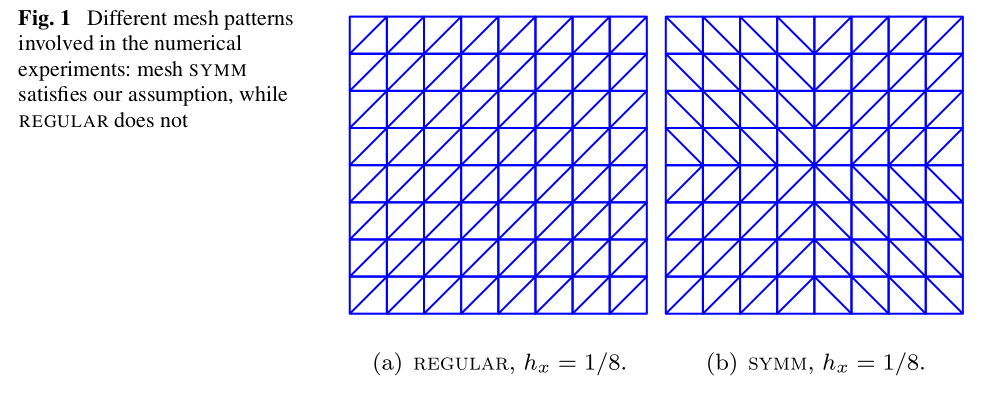
\includegraphics[width=10cm]{python_codes/fieldstone_120/images/bocg12}\\
{\captionfont Taken from \textcite{bocg12} (2012).}
\end{center} 


%-----------------------------------------------------------------------------
\subsection*{Finite element pairs for the Stokes equation}

\begin{center}
\begin{tabular}{p{1cm}p{2cm}p{4cm}p{2.5cm}p{5cm}}
\hline
 &pair & other name & information & remark \\
\hline
\hline
 1&${\bm Q}_1\times Q_0$   & ${\bm Q}_1\times P_0$  & Section~\ref{ss:pairq1p0} & NOT LBB STABLE but usable\\
 2&${\bm Q}_2\times Q_0$   &                  & Section~\ref{ss:pairq2q0}\\
 3&${\bm P}_2\times P_0$   &                  & Section~\ref{ss:p2p0}\\ 
 4&${\bm Q}_2\times Q_1$       &                  & Section~\ref{ss:pairq2q1}\\
 5&${\bm P}_2\times P_1$       &                  & Section~\ref{ss:p2p1}\\
 6&${\bm Q}_3\times Q_2$       &                  & Section~\ref{ss:q32d}\\
 7&${\bm P}_3\times P_2$       &                  & Section~\ref{ss:p3p2}\\
 8&${\bm Q}_1^+\times Q_1$     & Quad. MINI       & Section~\ref{ss:quadmini}\\
 9&${\bm P}_1^{+}\times P_{1}$ & MINI             & Section~\ref{pair:mini}\\
10&$RT_1\times Q_0$      &                  & Section~\ref{ss:RTq1p0}\\
11&$RT_2\times Q_0$      &                  & Section~\ref{ss:RTq1p0}\\
12&$DSSY_1\times Q_0$    &                  & Section~\ref{ss:pair_dssy2D}\\
13&$DSSY_2\times Q_0$    &                  & Section~\ref{ss:pair_dssy2D}\\
14&$Han\times Q_0$       &                  & Section~\ref{ss:han}\\
15&${\bm Q}_2\times P_{-1}$    &                  & Section~\ref{ss:pairq2pm1}\\
16&${\bm Q}_2\times P_{-1}(u)$ &                  & Section~\ref{ss:pairq2pm1}\\
17&${\bm Q}_2^{(8)}\times Q_1$ & Serendipity      & Section~\ref{sec:serendipity2D}\\
18&${\bm P}_2^+\times P_{-1}$  & Crouzeix-Raviart & Section~\ref{sec:crouzeix-raviart}\\
19&${\bm P}_2^+\times P_{1}$   &                  & Section~\ref{sec:p2pp1}\\
20&${\bm P}_2\times (P_1+P_0)$ & Augmented $P_2\times P_1$ & Section~\ref{ss:p2p1p0}\\
21&${\bm P}_1^{NC}\times P_0$  & Crouzeix-Raviart & Section~\ref{ss:p1ncp0}\\
22&${\bm P}_1\times P_0$       &                  & Section~\ref{ss:p1p0}  &NOT LBB STABLE and unusable\\
23&${\bm Q}_2\times Q_{-1}$    &                  & Section~\ref{ss:pair_q2qm1} & NOT LBB STABLE\\
24&${\bm Q}_2\times Q_1+Q_0$   & Augmented ${\bm Q}_2\times Q_1$ & Section~\ref{ss:pair_q2q1q0} \\
25&$Chen\times Q_0$      &                  & Section~\ref{ss:chenq0} & NOT SURE \\
26&${\bm Q}_4\times Q_3$       &                  & Section~\ref{ss:q42d}\\
27&${\bm P}_4\times P_3$       &                  & Section~\ref{ss:p42d}\\
\hline
\end{tabular}
\end{center}


{\bf Remark 2}: I have indeed built support for 3 unstable elements but 
these should not be included in the publication. 

{\bf Remark 3}: The augmented ${\bm P}_2\times (P_1+P_0)$ element pair is LBB stable 
but special care must be taken with respect to the rank-deficiency 
as explained in \textcite{bocg12} (2012). The same applies to ${\bm Q}_2\times (Q_1+Q_0)$. 
I propose a simple fix later. 

{\bf Remark 4}: The nonconforming ${\bm P}_1^{NC}\times P_0$ gives me a headache and does not 
yield accurate results (esp. the pressure). Not sure why... Coercivity/Korn stuff? I
have yet to find an article using the element 'as is'.

{\bf Remark 5} Following \textcite{john16} book, I could also do 
${\bm P}_3^+\times P_{-2}$, ${\bm Q}_3\times P_{-2}$. 

{\bf Remark 6}: A modified $Q_2$ Serendipity element was proposed by \textcite{zhxi20} (2020) 
(see Section~\ref{sec:serendipity2Db}) but it is only different from the standard serendipity 
element when the elements are not rectangles. 

{\bf Remark 7}: Using high-order element spaces ($Q_4$, $P_4$, ...) only makes sense in this context
if the manufactured solution is also a high-order polynomial or contains non-polynomial terms.

\vspace{0.5cm}

\begin{center}
Quadrilateral elements\\
\begin{tabular}{lcccccc}
\hline
Pspace $\downarrow$ / Vspace $\rightarrow$   
  & ${\bm Q}_1$  & ${\bm Q}_2$     & ${\bm Q}_2^{(8)}$ & ${\bm Q}_3$  & ${\bm Q}_4$ & ${\bm Q}_1^+$       \\ 
$Q_0$       & $\sqrt{}$ & $\sqrt{}$ & ?           & ?         &   & ?          \\
$Q_1$       & $\times$  & $\sqrt{}$ & $\sqrt{}$   & ?         &   & $\sqrt{}$  \\
$Q_2$       & $\times$  & $\times$  & $\times$    & $\sqrt{}$ &   & $\times$   \\
$Q_3$       & $\times$  & $\times$  & $\times$    & $\times$  & $\sqrt{}$ & $\times$ \\
$P_{-1}$    & ?         & $\sqrt{}$ & ?           & ?         &   & ?          \\
$P_{-1}(u)$ & ?         & $\sqrt{}$ & ?           & ?         &   & ?          \\
\hline
\end{tabular}
\end{center}

\begin{center}
Triangular elements\\
\begin{tabular}{cccccccc}
\hline
Pspace $\downarrow$ | Vspace $\rightarrow$   
         & ${\bm P}_1$    & ${\bm P}_2$     & ${\bm P}_3$     & ${\bm P}_4$    & ${\bm P}_1^+$   & ${\bm P}_2^+$   & ${\bm P}_1^{NC}$  \\
$P_0$    & $\times$ & $\sqrt{}$ & ?         & $\times$ &  ?        &  ?        & $\sqrt{}$   \\
$P_1$    & $\times$ & $\sqrt{}$ & ?         & $\times$ & $\sqrt{}$ &  ?        & ?           \\
$P_2$    & $\times$ & $\times$  & $\sqrt{}$ & $\times$ & $\times$  & $\times$  & $\times$    \\
$P_3$    & $\times$ & $\times$  & $\times$  & TODO     &           &           &             \\ 
$P_{-1}$ & $\times$ & $\sqrt{}$ & ?         &          &  ?        & $\sqrt{}$ & ?           \\
\hline
\end{tabular}
\end{center}

\newpage
%-----------------------------------


\begin{center}
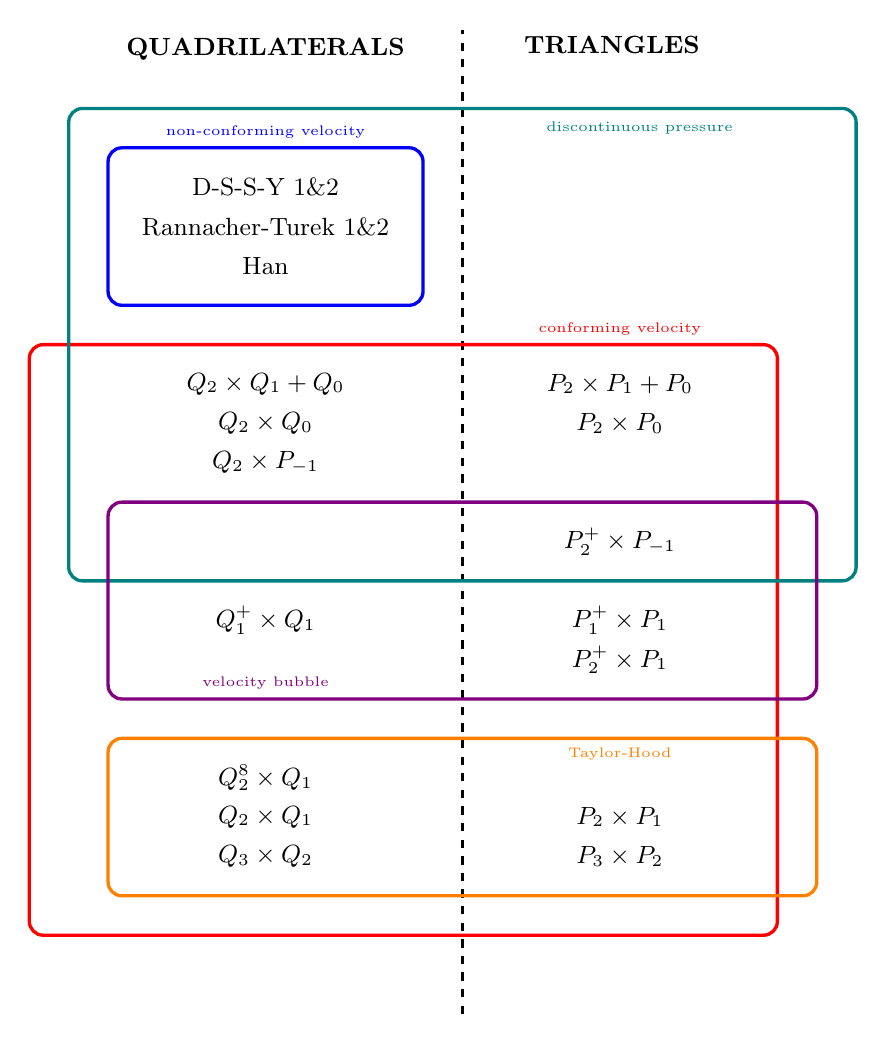
\begin{tikzpicture}
%\draw[step=0.5cm,gray,very thin] (0,0) grid (12,13); 

\node[] at (3,11.75) {\bf \small QUADRILATERALS};
\node[] at (7.4,11.8) {\bf \small TRIANGLES};

\draw[very thick,dashed](5.5,-0.5)--(5.5,12);

\node[] at (3,10) {\small D-S-S-Y 1\&2};
\node[] at (3,9.5) {\small Rannacher-Turek 1\&2};
\node[] at (3,9) {\small Han};
\node[] at (3,4.5) {\small $Q_1^+\times Q_1$};
\node[] at (3,2.5) {\small $Q_2^{8}\times Q_1$};

\node[] at (3,7.5) {\small $Q_2\times Q_1+Q_0$};
\node[] at (3,7) {\small $Q_2\times Q_0$};
\node[] at (3,6.5) {\small $Q_2\times P_{-1}$};

\node[] at (3,2) {\small $Q_2\times Q_1$};
\node[] at (3,1.5) {\small $Q_3\times Q_2$};

%triangles
\node[] at (7.5,7.5) {\small $P_2\times P_1+P_0$};
\node[] at (7.5,7) {\small $P_2\times P_0$};

\node[] at (7.5,5.5) {\small $P_2^+\times P_{-1}$};
\node[] at (7.5,4.5) {\small $P_1^+\times P_1$};
\node[] at (7.5,4) {\small $P_2^+\times P_1$};


\node[] at (7.5,2) {\small $P_2\times P_1$};
\node[] at (7.5,1.5) {\small $P_3\times P_2$};

\node[] at (7.5,8.2) {\tiny \color{red} conforming velocity};
\draw[rounded corners=5pt, very thick, red] (0,0.5) rectangle ++(9.5,7.5);

\node[] at (3,10.7) {\tiny \color{blue}non-conforming velocity};
\draw[rounded corners=5pt, very thick, blue] (1,8.5) rectangle ++(4,2);

\node[] at (7.75,10.75) {\tiny \color{teal}discontinuous pressure};
\draw[rounded corners=5pt, very thick, teal] (0.5,5) rectangle ++(10,6); % disc pressure

\node[] at (7.5,2.8) {\tiny \color{orange}Taylor-Hood};
\draw[rounded corners=5pt, very thick, orange] (1,1) rectangle ++(9,2);

\node[] at (3,3.7) {\tiny \color{violet} velocity bubble};
\draw[rounded corners=5pt, very thick, violet] (1,3.5) rectangle ++(9,2.5); %vel bubble

\end{tikzpicture}
\end{center}



$P_1^{nc} \times P_0$ belongs to non-conforming but it does not work.

\newpage
%-----------------------------------
\subsection*{The libraries}

There are three files which contain all the required tools to build most of a FE code:

\begin{itemize}

\item {\pythonfile FEbasis2D.py} contains 

\begin{itemize}
\item \lstinline{NNN(r,s,space)}: returns the basis functions $\bN_i (i=1,...m)$ at position $r,s$.
\item \lstinline{dNNNdr(r,s,space)}: returns basis function derivative $\partial_r\bN_i (i=1,...m)$ at position $r,s$.
\item \lstinline{dNNNds(r,s,space)}: returns basis function derivative $\partial_s\bN_i (i=1,...m)$ at position $r,s$.
\item \lstinline{NNN_r(space)}: returns the $r_i (i=1,...m)$ coordinates of the support nodes.
\item \lstinline{NNN_s(space)}: returns the $s_i (i=1,...m)$ coordinates of the support nodes.
\item \lstinline{NNN_m(space)}: returns the number of support nodes.
\item \lstinline{mapping(space)}: returns the type of mapping, i.e. $Q_1$ or $P_1$.
\item \lstinline{visualise_nodes(space)}: generates a png file with the support nodes and the shape of the reference element.
\item \lstinline{visualise_basis_functions(space)}: is an attempt at making a colormap of the basis functions.
\end{itemize}


\item {\pythonfile FEquadrature.py} contains
\begin{itemize}
\item \lstinline{quadrature(space,nqpts)}: it returns the number of quadrature points in the element, 
their coordinates and associated weights. If the element is a quadrilateral then it contains 
\lstinline{nqpts}$\times$\lstinline{nqpts} quadrature points. 
If it is a triangle then it contains \lstinline{nqpts} quadrature points in total. 
In that case only 3,6,7,12,13,16 are authorized.   
\item \lstinline{qcoords_1D(nqpts)}: returns the coordinates of the \lstinline{nqpts} quadrature points between -1 and 1.
\item \lstinline{qweights_1D(nqpts)}:returns the weights of the \lstinline{nqpts} quadrature points.
\item \lstinline{visualise_quadrature_points(space,nqpts)}: generates a png file.
\end{itemize}


\item {\pythonfile FEtools.py} contains

\begin{itemize}
\item \lstinline{cartesian_mesh(Lx,Ly,nelx,nely,space)}: Creates a cartesian mesh of \lstinline{nelx}
$\times$\lstinline{nely} elements in the domain $[0,L_x]\times[0,L_y]$. It returns the total 
number of nodes \lstinline{N}, the number of elements \lstinline{nel}, the coordinates of all the 
nodes in \lstinline{x,y} arrays and the connectivity array \lstinline{icon}.
\item \lstinline{randomize_background_mesh(x1,y1,hx,hy,N1,Lx,Ly)}: this adds a random perturbation
to the coordinates of all the nodes of the background mesh inside the domain (i.e. not on the boundary!). 
The amplitude of the perturbation is bounded by $0.1h_x$ and $0.1h_y$ in the $x$ and $y$ direction.
\item \lstinline{adapt_FE_mesh(x1,y1,icon1,m1,space1,x,y,icon,nel,space)}: This makes sure that 
all the support nodes for a given space are displaced so as to follow the randomized 
background mesh, using a (bi-)linear mapping.

\item \lstinline{export_swarm_to_ascii(x,y,filename)}:
\item \lstinline{export_swarm_scalar_to_ascii(x,y,f,filename)}:
\item \lstinline{export_swarm_vector_to_ascii(x,y,u,v,filename)}:
\item \lstinline{export_connectivity_array_to_ascii(x,y,icon,filename)}:
\item \lstinline{export_elements_to_vtu(x,y,icon,space,filename)}:
\item \lstinline{export_swarm_to_vtu(x,y,filename)}:
\item \lstinline{export_swarm_vector_to_vtu(x,y,vx,vy,filename)}:
\item \lstinline{export_swarm_scalar_to_vtu(x,y,scalar,filename)}:
\item \lstinline{bc_setup(x,y,Lx,Ly,ndof,left,right,bottom,top)}:
\item \lstinline{J(m,dNdr,dNds,x,y)}: computes the Jacobian matrix and its determinant 
for the mapping. 
\item \lstinline{assemble_K(K_el,A_sparse,iconV,mV,ndofV,iel)}:
\item \lstinline{assemble_G(G_el,A_sparse,iconV,iconP,NfemV,mV,mP,ndofV,ndofP,iel)}:
\item \lstinline{assemble_f(f_el,rhs,iconV,mV,ndofV,iel)}:
\item \lstinline{apply_bc(K_el,G_el,f_el,h_el,bc_val,bc_fix,iconV,mV,ndofV,iel)}:
\item \lstinline{visualise_with_tikz(x,y,space)}: generates a .tex file containing 
a tikz drawing of the nodes layout. Only works for 3x3 meshes. 
\end{itemize}

\end{itemize}

\newpage
%--------------------------------------------------------------------
\subsection*{Supported element spaces}

These figures are obtained by running \lstinline{tester6.py}.

\begin{center}
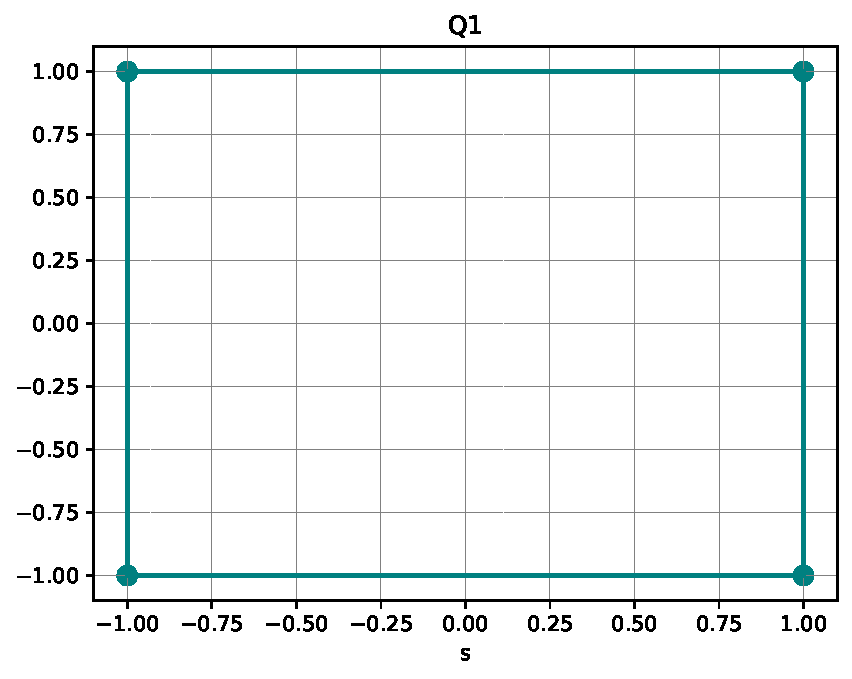
\includegraphics[width=4cm]{python_codes/fieldstone_120/spaces/Q1_nodes}
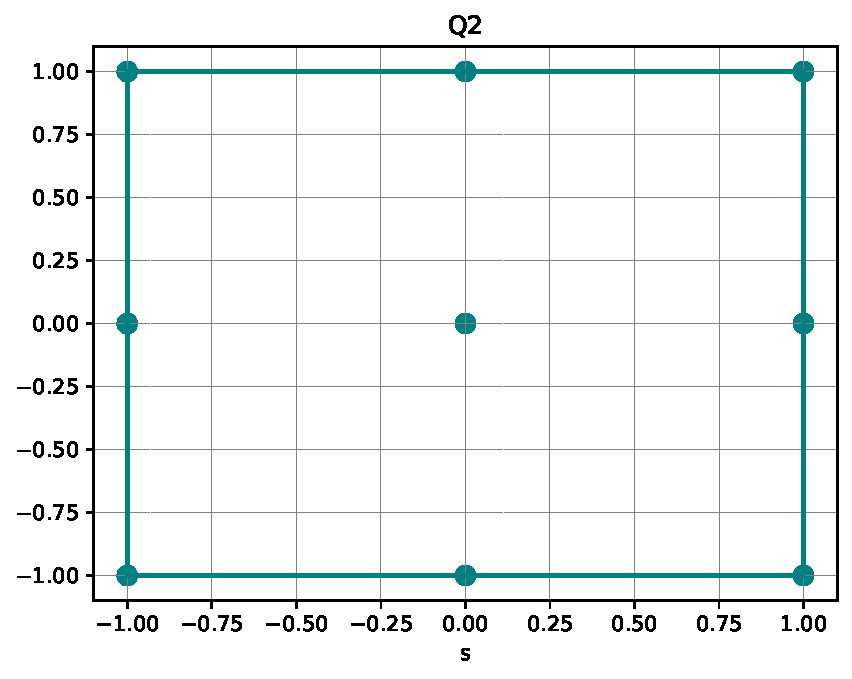
\includegraphics[width=4cm]{python_codes/fieldstone_120/spaces/Q2_nodes}
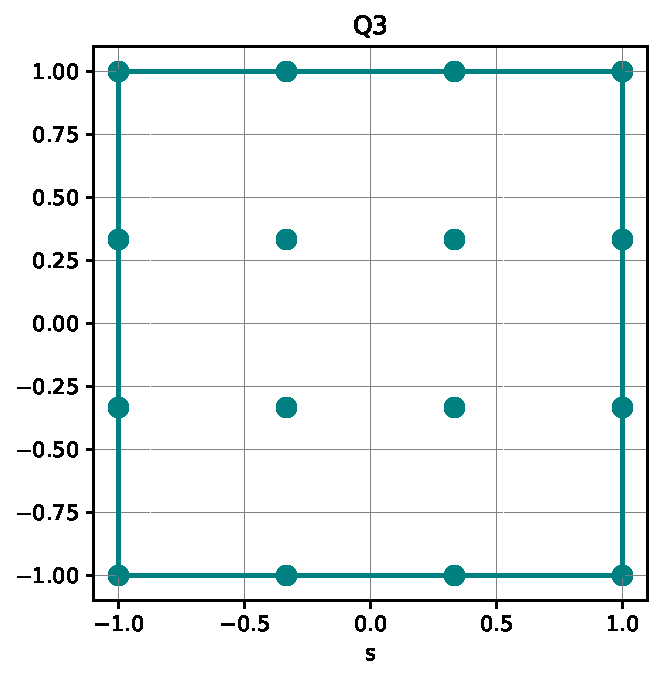
\includegraphics[width=4cm]{python_codes/fieldstone_120/spaces/Q3_nodes}
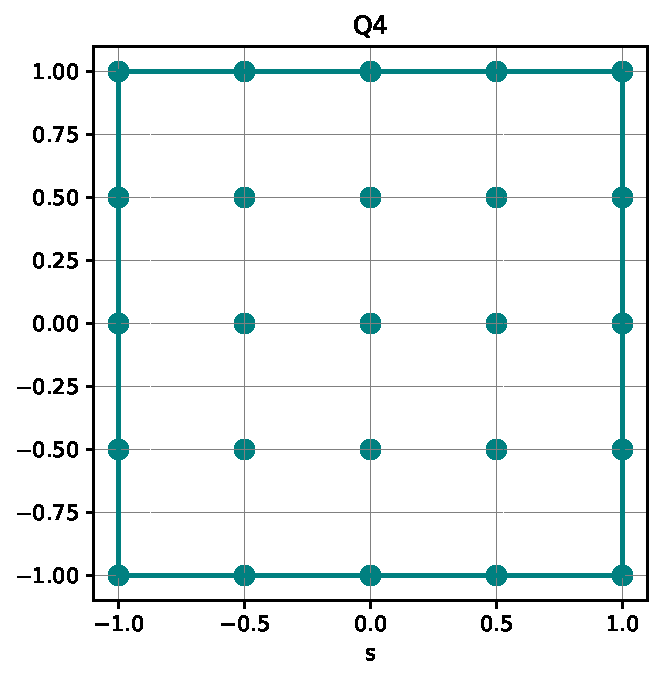
\includegraphics[width=4cm]{python_codes/fieldstone_120/spaces/Q4_nodes}\\
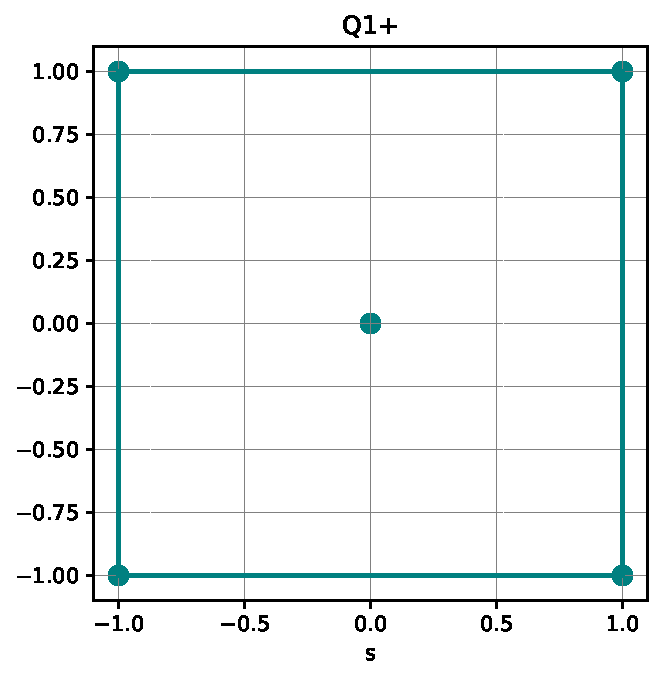
\includegraphics[width=4cm]{python_codes/fieldstone_120/spaces/Q1+_nodes}
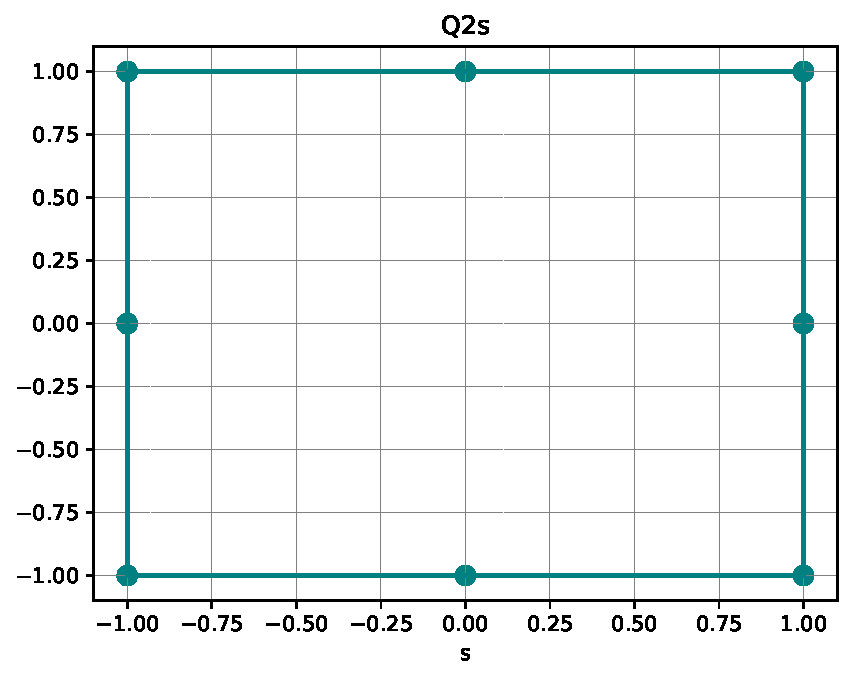
\includegraphics[width=4cm]{python_codes/fieldstone_120/spaces/Q2s_nodes}
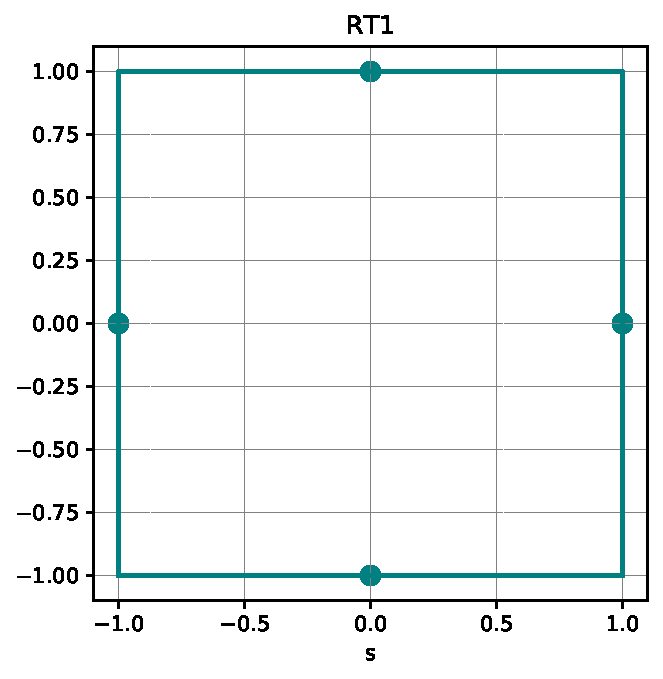
\includegraphics[width=4cm]{python_codes/fieldstone_120/spaces/RT1_nodes}
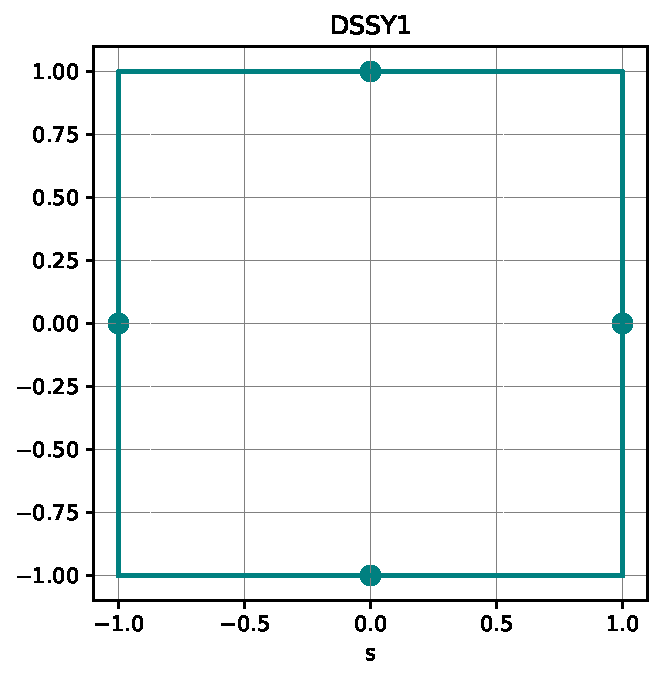
\includegraphics[width=4cm]{python_codes/fieldstone_120/spaces/DSSY1_nodes}\\
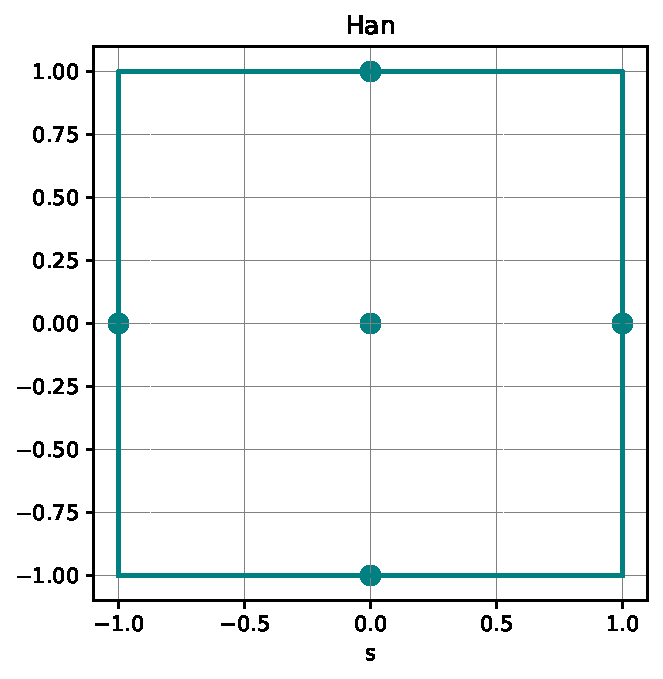
\includegraphics[width=4cm]{python_codes/fieldstone_120/spaces/Han_nodes}\\
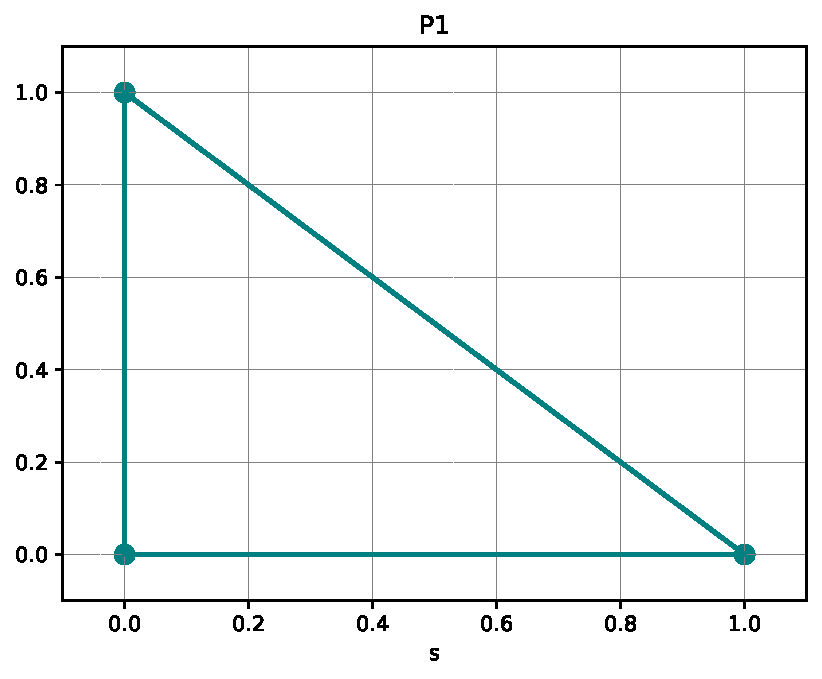
\includegraphics[width=4cm]{python_codes/fieldstone_120/spaces/P1_nodes}
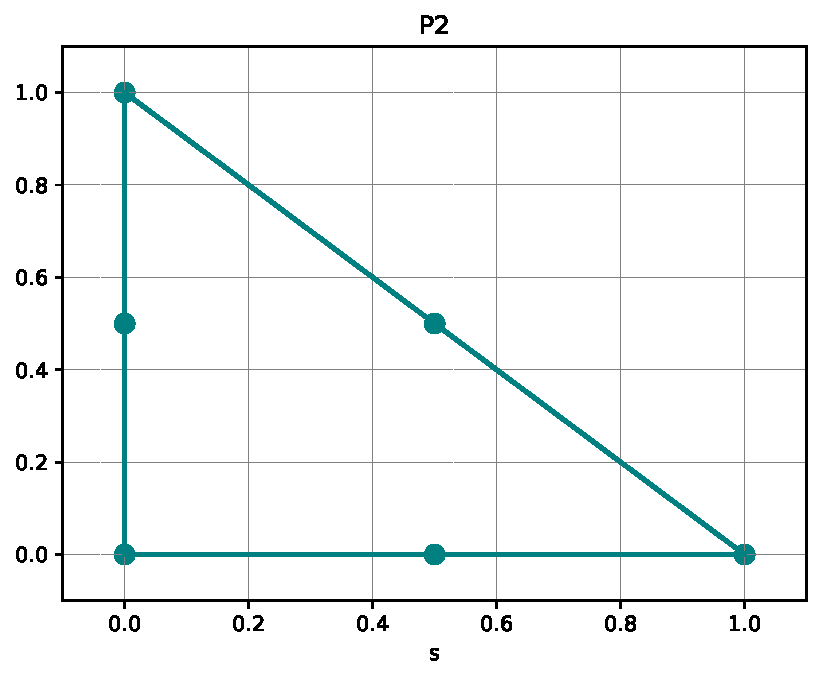
\includegraphics[width=4cm]{python_codes/fieldstone_120/spaces/P2_nodes}
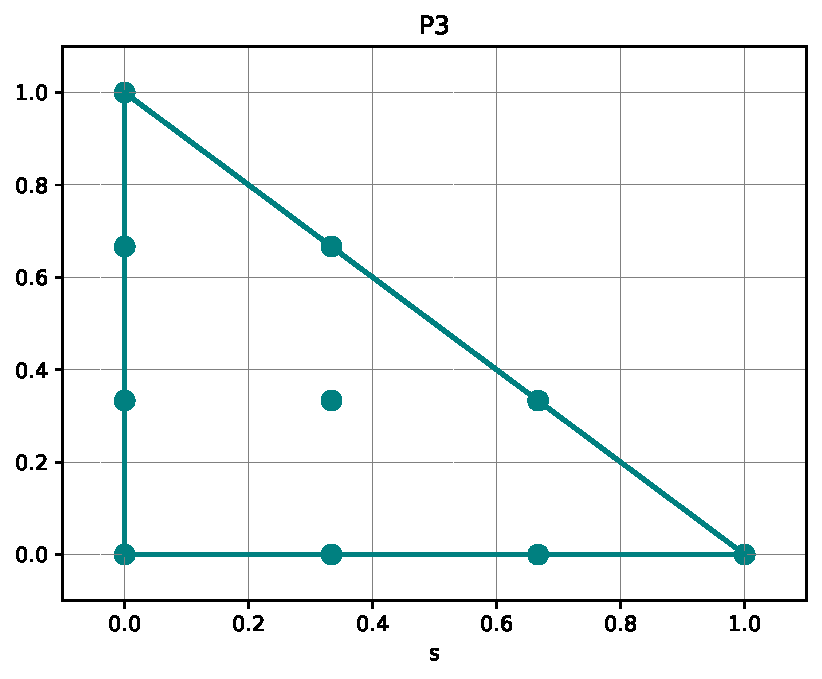
\includegraphics[width=4cm]{python_codes/fieldstone_120/spaces/P3_nodes}
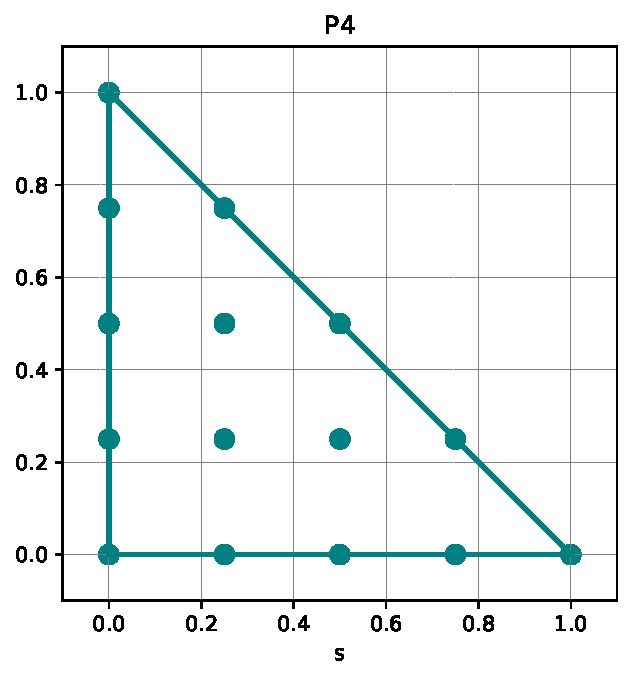
\includegraphics[width=4cm]{python_codes/fieldstone_120/spaces/P4_nodes}
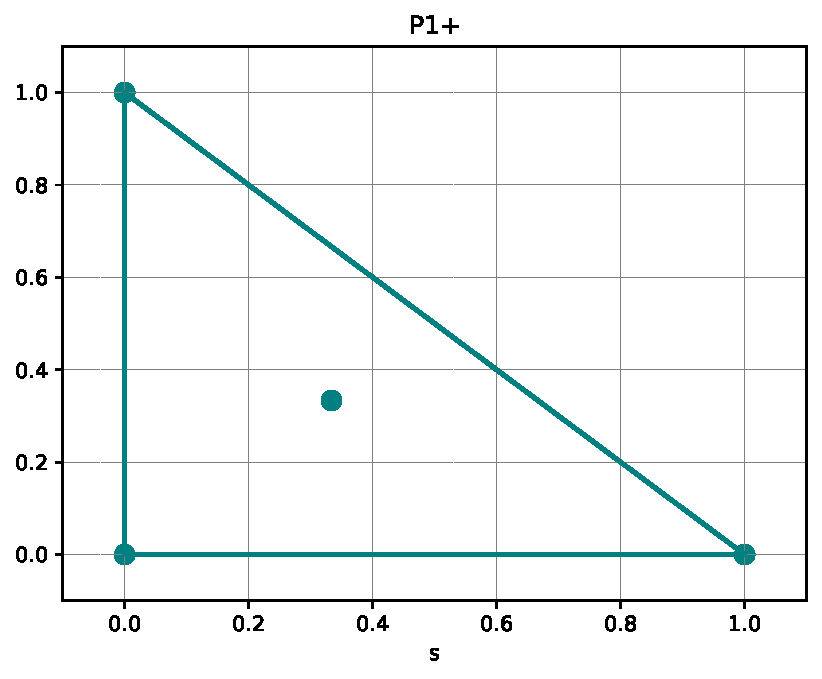
\includegraphics[width=4cm]{python_codes/fieldstone_120/spaces/P1+_nodes}\\
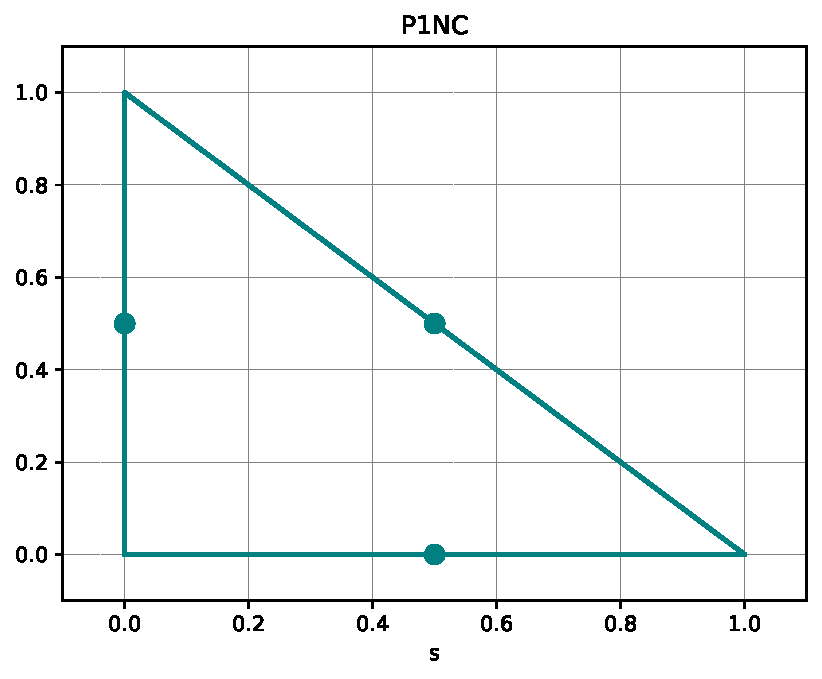
\includegraphics[width=4cm]{python_codes/fieldstone_120/spaces/P1NC_nodes}
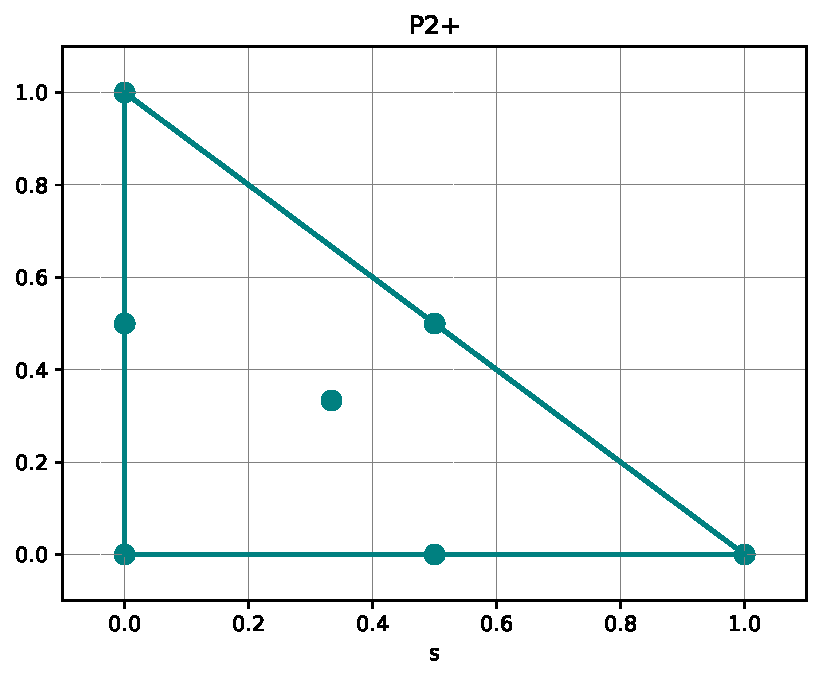
\includegraphics[width=4cm]{python_codes/fieldstone_120/spaces/P2+_nodes}
\end{center}

\newpage
%--------------------------------------------------------------------
\subsection*{$3\times 2$ meshes with velocity nodes}

%------------------
\begin{multicols}{2}
\begin{center} 
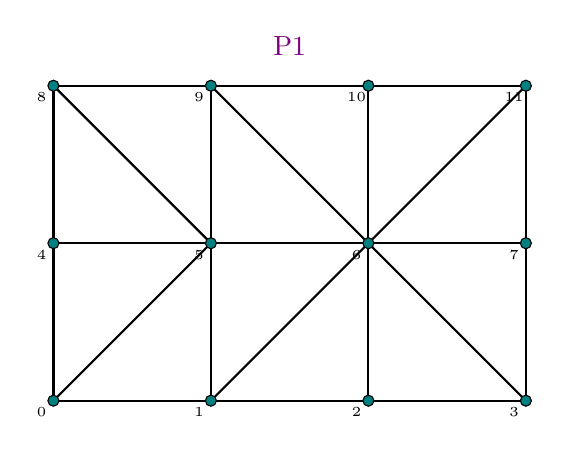
\begin{tikzpicture} 
\node[violet] at (3,4.5) {P1}; 
\draw[thick] (0,0) -- (6,0) -- (6,4) -- (0,4) -- cycle; 
\draw[thick] (0,2) -- (6,2) ; 
\draw[thick] (2,0) -- (2,4) ; 
\draw[thick] (4,0) -- (4,4) ; 
\draw[thick] (0,0) -- (2,2) -- (0,4) ; 
\draw[thick] (2,0) -- (4,2) -- (2,4) ; 
\draw[thick] (6,0) -- (4,2) -- (6,4) ; 
\draw[black,fill=teal] ( 0.000000 , 0.000000)     circle (2pt); 
\node[] at ( -0.150000, -0.150000 ) {\tiny 0 }; 
\draw[black,fill=teal] ( 2.000000 , 0.000000)     circle (2pt); 
\node[] at ( 1.850000, -0.150000 ) {\tiny 1 }; 
\draw[black,fill=teal] ( 4.000000 , 0.000000)     circle (2pt); 
\node[] at ( 3.850000, -0.150000 ) {\tiny 2 }; 
\draw[black,fill=teal] ( 6.000000 , 0.000000)     circle (2pt); 
\node[] at ( 5.850000, -0.150000 ) {\tiny 3 }; 
\draw[black,fill=teal] ( 0.000000 , 2.000000)     circle (2pt); 
\node[] at ( -0.150000, 1.850000 ) {\tiny 4 }; 
\draw[black,fill=teal] ( 2.000000 , 2.000000)     circle (2pt); 
\node[] at ( 1.850000, 1.850000 ) {\tiny 5 }; 
\draw[black,fill=teal] ( 4.000000 , 2.000000)     circle (2pt); 
\node[] at ( 3.850000, 1.850000 ) {\tiny 6 }; 
\draw[black,fill=teal] ( 6.000000 , 2.000000)     circle (2pt); 
\node[] at ( 5.850000, 1.850000 ) {\tiny 7 }; 
\draw[black,fill=teal] ( 0.000000 , 4.000000)     circle (2pt); 
\node[] at ( -0.150000, 3.850000 ) {\tiny 8 }; 
\draw[black,fill=teal] ( 2.000000 , 4.000000)     circle (2pt); 
\node[] at ( 1.850000, 3.850000 ) {\tiny 9 }; 
\draw[black,fill=teal] ( 4.000000 , 4.000000)     circle (2pt); 
\node[] at ( 3.850000, 3.850000 ) {\tiny 10 }; 
\draw[black,fill=teal] ( 6.000000 , 4.000000)     circle (2pt); 
\node[] at ( 5.850000, 3.850000 ) {\tiny 11 }; 
\end{tikzpicture} 
\end{center} 


\begin{tiny}
\verbatiminput{python_codes/fieldstone_120/spaces/iconV_elt1_P1.ascii}
\end{tiny}
\end{multicols}

%------------------
\begin{multicols}{2}
\begin{center} 
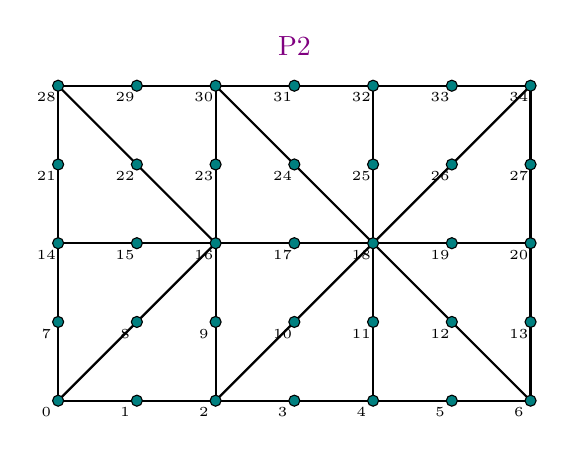
\begin{tikzpicture} 
\node[violet] at (3,4.5) {P2}; 
\draw[thick] (0,0) -- (6,0) -- (6,4) -- (0,4) -- cycle; 
\draw[thick] (0,2) -- (6,2) ; 
\draw[thick] (2,0) -- (2,4) ; 
\draw[thick] (4,0) -- (4,4) ; 
\draw[thick] (0,0) -- (2,2) -- (0,4) ; 
\draw[thick] (2,0) -- (4,2) -- (2,4) ; 
\draw[thick] (6,0) -- (4,2) -- (6,4) ; 
\draw[black,fill=teal] ( 0.000000 , 0.000000)     circle (2pt); 
\node[] at ( -0.150000, -0.150000 ) {\tiny 0 }; 
\draw[black,fill=teal] ( 1.000000 , 0.000000)     circle (2pt); 
\node[] at ( 0.850000, -0.150000 ) {\tiny 1 }; 
\draw[black,fill=teal] ( 2.000000 , 0.000000)     circle (2pt); 
\node[] at ( 1.850000, -0.150000 ) {\tiny 2 }; 
\draw[black,fill=teal] ( 3.000000 , 0.000000)     circle (2pt); 
\node[] at ( 2.850000, -0.150000 ) {\tiny 3 }; 
\draw[black,fill=teal] ( 4.000000 , 0.000000)     circle (2pt); 
\node[] at ( 3.850000, -0.150000 ) {\tiny 4 }; 
\draw[black,fill=teal] ( 5.000000 , 0.000000)     circle (2pt); 
\node[] at ( 4.850000, -0.150000 ) {\tiny 5 }; 
\draw[black,fill=teal] ( 6.000000 , 0.000000)     circle (2pt); 
\node[] at ( 5.850000, -0.150000 ) {\tiny 6 }; 
\draw[black,fill=teal] ( 0.000000 , 1.000000)     circle (2pt); 
\node[] at ( -0.150000, 0.850000 ) {\tiny 7 }; 
\draw[black,fill=teal] ( 1.000000 , 1.000000)     circle (2pt); 
\node[] at ( 0.850000, 0.850000 ) {\tiny 8 }; 
\draw[black,fill=teal] ( 2.000000 , 1.000000)     circle (2pt); 
\node[] at ( 1.850000, 0.850000 ) {\tiny 9 }; 
\draw[black,fill=teal] ( 3.000000 , 1.000000)     circle (2pt); 
\node[] at ( 2.850000, 0.850000 ) {\tiny 10 }; 
\draw[black,fill=teal] ( 4.000000 , 1.000000)     circle (2pt); 
\node[] at ( 3.850000, 0.850000 ) {\tiny 11 }; 
\draw[black,fill=teal] ( 5.000000 , 1.000000)     circle (2pt); 
\node[] at ( 4.850000, 0.850000 ) {\tiny 12 }; 
\draw[black,fill=teal] ( 6.000000 , 1.000000)     circle (2pt); 
\node[] at ( 5.850000, 0.850000 ) {\tiny 13 }; 
\draw[black,fill=teal] ( 0.000000 , 2.000000)     circle (2pt); 
\node[] at ( -0.150000, 1.850000 ) {\tiny 14 }; 
\draw[black,fill=teal] ( 1.000000 , 2.000000)     circle (2pt); 
\node[] at ( 0.850000, 1.850000 ) {\tiny 15 }; 
\draw[black,fill=teal] ( 2.000000 , 2.000000)     circle (2pt); 
\node[] at ( 1.850000, 1.850000 ) {\tiny 16 }; 
\draw[black,fill=teal] ( 3.000000 , 2.000000)     circle (2pt); 
\node[] at ( 2.850000, 1.850000 ) {\tiny 17 }; 
\draw[black,fill=teal] ( 4.000000 , 2.000000)     circle (2pt); 
\node[] at ( 3.850000, 1.850000 ) {\tiny 18 }; 
\draw[black,fill=teal] ( 5.000000 , 2.000000)     circle (2pt); 
\node[] at ( 4.850000, 1.850000 ) {\tiny 19 }; 
\draw[black,fill=teal] ( 6.000000 , 2.000000)     circle (2pt); 
\node[] at ( 5.850000, 1.850000 ) {\tiny 20 }; 
\draw[black,fill=teal] ( 0.000000 , 3.000000)     circle (2pt); 
\node[] at ( -0.150000, 2.850000 ) {\tiny 21 }; 
\draw[black,fill=teal] ( 1.000000 , 3.000000)     circle (2pt); 
\node[] at ( 0.850000, 2.850000 ) {\tiny 22 }; 
\draw[black,fill=teal] ( 2.000000 , 3.000000)     circle (2pt); 
\node[] at ( 1.850000, 2.850000 ) {\tiny 23 }; 
\draw[black,fill=teal] ( 3.000000 , 3.000000)     circle (2pt); 
\node[] at ( 2.850000, 2.850000 ) {\tiny 24 }; 
\draw[black,fill=teal] ( 4.000000 , 3.000000)     circle (2pt); 
\node[] at ( 3.850000, 2.850000 ) {\tiny 25 }; 
\draw[black,fill=teal] ( 5.000000 , 3.000000)     circle (2pt); 
\node[] at ( 4.850000, 2.850000 ) {\tiny 26 }; 
\draw[black,fill=teal] ( 6.000000 , 3.000000)     circle (2pt); 
\node[] at ( 5.850000, 2.850000 ) {\tiny 27 }; 
\draw[black,fill=teal] ( 0.000000 , 4.000000)     circle (2pt); 
\node[] at ( -0.150000, 3.850000 ) {\tiny 28 }; 
\draw[black,fill=teal] ( 1.000000 , 4.000000)     circle (2pt); 
\node[] at ( 0.850000, 3.850000 ) {\tiny 29 }; 
\draw[black,fill=teal] ( 2.000000 , 4.000000)     circle (2pt); 
\node[] at ( 1.850000, 3.850000 ) {\tiny 30 }; 
\draw[black,fill=teal] ( 3.000000 , 4.000000)     circle (2pt); 
\node[] at ( 2.850000, 3.850000 ) {\tiny 31 }; 
\draw[black,fill=teal] ( 4.000000 , 4.000000)     circle (2pt); 
\node[] at ( 3.850000, 3.850000 ) {\tiny 32 }; 
\draw[black,fill=teal] ( 5.000000 , 4.000000)     circle (2pt); 
\node[] at ( 4.850000, 3.850000 ) {\tiny 33 }; 
\draw[black,fill=teal] ( 6.000000 , 4.000000)     circle (2pt); 
\node[] at ( 5.850000, 3.850000 ) {\tiny 34 }; 
\end{tikzpicture} 
\end{center} 


\begin{tiny}
\verbatiminput{python_codes/fieldstone_120/spaces/iconV_elt1_P2.ascii}
\end{tiny}
\end{multicols}

%------------------
\begin{multicols}{2}
\begin{center} 
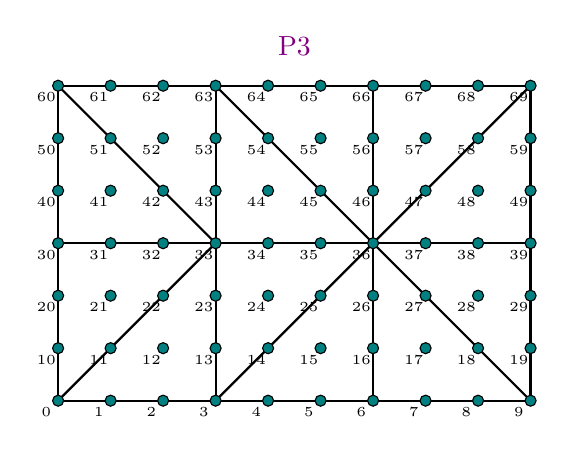
\begin{tikzpicture} 
\node[violet] at (3,4.5) {P3}; 
\draw[thick] (0,0) -- (6,0) -- (6,4) -- (0,4) -- cycle; 
\draw[thick] (0,2) -- (6,2) ; 
\draw[thick] (2,0) -- (2,4) ; 
\draw[thick] (4,0) -- (4,4) ; 
\draw[thick] (0,0) -- (2,2) -- (0,4) ; 
\draw[thick] (2,0) -- (4,2) -- (2,4) ; 
\draw[thick] (6,0) -- (4,2) -- (6,4) ; 
\draw[black,fill=teal] ( 0.000000 , 0.000000)     circle (2pt); 
\node[] at ( -0.150000, -0.150000 ) {\tiny 0 }; 
\draw[black,fill=teal] ( 0.666667 , 0.000000)     circle (2pt); 
\node[] at ( 0.516667, -0.150000 ) {\tiny 1 }; 
\draw[black,fill=teal] ( 1.333333 , 0.000000)     circle (2pt); 
\node[] at ( 1.183333, -0.150000 ) {\tiny 2 }; 
\draw[black,fill=teal] ( 2.000000 , 0.000000)     circle (2pt); 
\node[] at ( 1.850000, -0.150000 ) {\tiny 3 }; 
\draw[black,fill=teal] ( 2.666667 , 0.000000)     circle (2pt); 
\node[] at ( 2.516667, -0.150000 ) {\tiny 4 }; 
\draw[black,fill=teal] ( 3.333333 , 0.000000)     circle (2pt); 
\node[] at ( 3.183333, -0.150000 ) {\tiny 5 }; 
\draw[black,fill=teal] ( 4.000000 , 0.000000)     circle (2pt); 
\node[] at ( 3.850000, -0.150000 ) {\tiny 6 }; 
\draw[black,fill=teal] ( 4.666667 , 0.000000)     circle (2pt); 
\node[] at ( 4.516667, -0.150000 ) {\tiny 7 }; 
\draw[black,fill=teal] ( 5.333333 , 0.000000)     circle (2pt); 
\node[] at ( 5.183333, -0.150000 ) {\tiny 8 }; 
\draw[black,fill=teal] ( 6.000000 , 0.000000)     circle (2pt); 
\node[] at ( 5.850000, -0.150000 ) {\tiny 9 }; 
\draw[black,fill=teal] ( 0.000000 , 0.666667)     circle (2pt); 
\node[] at ( -0.150000, 0.516667 ) {\tiny 10 }; 
\draw[black,fill=teal] ( 0.666667 , 0.666667)     circle (2pt); 
\node[] at ( 0.516667, 0.516667 ) {\tiny 11 }; 
\draw[black,fill=teal] ( 1.333333 , 0.666667)     circle (2pt); 
\node[] at ( 1.183333, 0.516667 ) {\tiny 12 }; 
\draw[black,fill=teal] ( 2.000000 , 0.666667)     circle (2pt); 
\node[] at ( 1.850000, 0.516667 ) {\tiny 13 }; 
\draw[black,fill=teal] ( 2.666667 , 0.666667)     circle (2pt); 
\node[] at ( 2.516667, 0.516667 ) {\tiny 14 }; 
\draw[black,fill=teal] ( 3.333333 , 0.666667)     circle (2pt); 
\node[] at ( 3.183333, 0.516667 ) {\tiny 15 }; 
\draw[black,fill=teal] ( 4.000000 , 0.666667)     circle (2pt); 
\node[] at ( 3.850000, 0.516667 ) {\tiny 16 }; 
\draw[black,fill=teal] ( 4.666667 , 0.666667)     circle (2pt); 
\node[] at ( 4.516667, 0.516667 ) {\tiny 17 }; 
\draw[black,fill=teal] ( 5.333333 , 0.666667)     circle (2pt); 
\node[] at ( 5.183333, 0.516667 ) {\tiny 18 }; 
\draw[black,fill=teal] ( 6.000000 , 0.666667)     circle (2pt); 
\node[] at ( 5.850000, 0.516667 ) {\tiny 19 }; 
\draw[black,fill=teal] ( 0.000000 , 1.333333)     circle (2pt); 
\node[] at ( -0.150000, 1.183333 ) {\tiny 20 }; 
\draw[black,fill=teal] ( 0.666667 , 1.333333)     circle (2pt); 
\node[] at ( 0.516667, 1.183333 ) {\tiny 21 }; 
\draw[black,fill=teal] ( 1.333333 , 1.333333)     circle (2pt); 
\node[] at ( 1.183333, 1.183333 ) {\tiny 22 }; 
\draw[black,fill=teal] ( 2.000000 , 1.333333)     circle (2pt); 
\node[] at ( 1.850000, 1.183333 ) {\tiny 23 }; 
\draw[black,fill=teal] ( 2.666667 , 1.333333)     circle (2pt); 
\node[] at ( 2.516667, 1.183333 ) {\tiny 24 }; 
\draw[black,fill=teal] ( 3.333333 , 1.333333)     circle (2pt); 
\node[] at ( 3.183333, 1.183333 ) {\tiny 25 }; 
\draw[black,fill=teal] ( 4.000000 , 1.333333)     circle (2pt); 
\node[] at ( 3.850000, 1.183333 ) {\tiny 26 }; 
\draw[black,fill=teal] ( 4.666667 , 1.333333)     circle (2pt); 
\node[] at ( 4.516667, 1.183333 ) {\tiny 27 }; 
\draw[black,fill=teal] ( 5.333333 , 1.333333)     circle (2pt); 
\node[] at ( 5.183333, 1.183333 ) {\tiny 28 }; 
\draw[black,fill=teal] ( 6.000000 , 1.333333)     circle (2pt); 
\node[] at ( 5.850000, 1.183333 ) {\tiny 29 }; 
\draw[black,fill=teal] ( 0.000000 , 2.000000)     circle (2pt); 
\node[] at ( -0.150000, 1.850000 ) {\tiny 30 }; 
\draw[black,fill=teal] ( 0.666667 , 2.000000)     circle (2pt); 
\node[] at ( 0.516667, 1.850000 ) {\tiny 31 }; 
\draw[black,fill=teal] ( 1.333333 , 2.000000)     circle (2pt); 
\node[] at ( 1.183333, 1.850000 ) {\tiny 32 }; 
\draw[black,fill=teal] ( 2.000000 , 2.000000)     circle (2pt); 
\node[] at ( 1.850000, 1.850000 ) {\tiny 33 }; 
\draw[black,fill=teal] ( 2.666667 , 2.000000)     circle (2pt); 
\node[] at ( 2.516667, 1.850000 ) {\tiny 34 }; 
\draw[black,fill=teal] ( 3.333333 , 2.000000)     circle (2pt); 
\node[] at ( 3.183333, 1.850000 ) {\tiny 35 }; 
\draw[black,fill=teal] ( 4.000000 , 2.000000)     circle (2pt); 
\node[] at ( 3.850000, 1.850000 ) {\tiny 36 }; 
\draw[black,fill=teal] ( 4.666667 , 2.000000)     circle (2pt); 
\node[] at ( 4.516667, 1.850000 ) {\tiny 37 }; 
\draw[black,fill=teal] ( 5.333333 , 2.000000)     circle (2pt); 
\node[] at ( 5.183333, 1.850000 ) {\tiny 38 }; 
\draw[black,fill=teal] ( 6.000000 , 2.000000)     circle (2pt); 
\node[] at ( 5.850000, 1.850000 ) {\tiny 39 }; 
\draw[black,fill=teal] ( 0.000000 , 2.666667)     circle (2pt); 
\node[] at ( -0.150000, 2.516667 ) {\tiny 40 }; 
\draw[black,fill=teal] ( 0.666667 , 2.666667)     circle (2pt); 
\node[] at ( 0.516667, 2.516667 ) {\tiny 41 }; 
\draw[black,fill=teal] ( 1.333333 , 2.666667)     circle (2pt); 
\node[] at ( 1.183333, 2.516667 ) {\tiny 42 }; 
\draw[black,fill=teal] ( 2.000000 , 2.666667)     circle (2pt); 
\node[] at ( 1.850000, 2.516667 ) {\tiny 43 }; 
\draw[black,fill=teal] ( 2.666667 , 2.666667)     circle (2pt); 
\node[] at ( 2.516667, 2.516667 ) {\tiny 44 }; 
\draw[black,fill=teal] ( 3.333333 , 2.666667)     circle (2pt); 
\node[] at ( 3.183333, 2.516667 ) {\tiny 45 }; 
\draw[black,fill=teal] ( 4.000000 , 2.666667)     circle (2pt); 
\node[] at ( 3.850000, 2.516667 ) {\tiny 46 }; 
\draw[black,fill=teal] ( 4.666667 , 2.666667)     circle (2pt); 
\node[] at ( 4.516667, 2.516667 ) {\tiny 47 }; 
\draw[black,fill=teal] ( 5.333333 , 2.666667)     circle (2pt); 
\node[] at ( 5.183333, 2.516667 ) {\tiny 48 }; 
\draw[black,fill=teal] ( 6.000000 , 2.666667)     circle (2pt); 
\node[] at ( 5.850000, 2.516667 ) {\tiny 49 }; 
\draw[black,fill=teal] ( 0.000000 , 3.333333)     circle (2pt); 
\node[] at ( -0.150000, 3.183333 ) {\tiny 50 }; 
\draw[black,fill=teal] ( 0.666667 , 3.333333)     circle (2pt); 
\node[] at ( 0.516667, 3.183333 ) {\tiny 51 }; 
\draw[black,fill=teal] ( 1.333333 , 3.333333)     circle (2pt); 
\node[] at ( 1.183333, 3.183333 ) {\tiny 52 }; 
\draw[black,fill=teal] ( 2.000000 , 3.333333)     circle (2pt); 
\node[] at ( 1.850000, 3.183333 ) {\tiny 53 }; 
\draw[black,fill=teal] ( 2.666667 , 3.333333)     circle (2pt); 
\node[] at ( 2.516667, 3.183333 ) {\tiny 54 }; 
\draw[black,fill=teal] ( 3.333333 , 3.333333)     circle (2pt); 
\node[] at ( 3.183333, 3.183333 ) {\tiny 55 }; 
\draw[black,fill=teal] ( 4.000000 , 3.333333)     circle (2pt); 
\node[] at ( 3.850000, 3.183333 ) {\tiny 56 }; 
\draw[black,fill=teal] ( 4.666667 , 3.333333)     circle (2pt); 
\node[] at ( 4.516667, 3.183333 ) {\tiny 57 }; 
\draw[black,fill=teal] ( 5.333333 , 3.333333)     circle (2pt); 
\node[] at ( 5.183333, 3.183333 ) {\tiny 58 }; 
\draw[black,fill=teal] ( 6.000000 , 3.333333)     circle (2pt); 
\node[] at ( 5.850000, 3.183333 ) {\tiny 59 }; 
\draw[black,fill=teal] ( 0.000000 , 4.000000)     circle (2pt); 
\node[] at ( -0.150000, 3.850000 ) {\tiny 60 }; 
\draw[black,fill=teal] ( 0.666667 , 4.000000)     circle (2pt); 
\node[] at ( 0.516667, 3.850000 ) {\tiny 61 }; 
\draw[black,fill=teal] ( 1.333333 , 4.000000)     circle (2pt); 
\node[] at ( 1.183333, 3.850000 ) {\tiny 62 }; 
\draw[black,fill=teal] ( 2.000000 , 4.000000)     circle (2pt); 
\node[] at ( 1.850000, 3.850000 ) {\tiny 63 }; 
\draw[black,fill=teal] ( 2.666667 , 4.000000)     circle (2pt); 
\node[] at ( 2.516667, 3.850000 ) {\tiny 64 }; 
\draw[black,fill=teal] ( 3.333333 , 4.000000)     circle (2pt); 
\node[] at ( 3.183333, 3.850000 ) {\tiny 65 }; 
\draw[black,fill=teal] ( 4.000000 , 4.000000)     circle (2pt); 
\node[] at ( 3.850000, 3.850000 ) {\tiny 66 }; 
\draw[black,fill=teal] ( 4.666667 , 4.000000)     circle (2pt); 
\node[] at ( 4.516667, 3.850000 ) {\tiny 67 }; 
\draw[black,fill=teal] ( 5.333333 , 4.000000)     circle (2pt); 
\node[] at ( 5.183333, 3.850000 ) {\tiny 68 }; 
\draw[black,fill=teal] ( 6.000000 , 4.000000)     circle (2pt); 
\node[] at ( 5.850000, 3.850000 ) {\tiny 69 }; 
\end{tikzpicture} 
\end{center} 


\begin{tiny}
\verbatiminput{python_codes/fieldstone_120/spaces/iconV_elt1_P3.ascii}
\end{tiny}
\end{multicols}

\newpage
%------------------
\begin{multicols}{2}
\begin{center} 
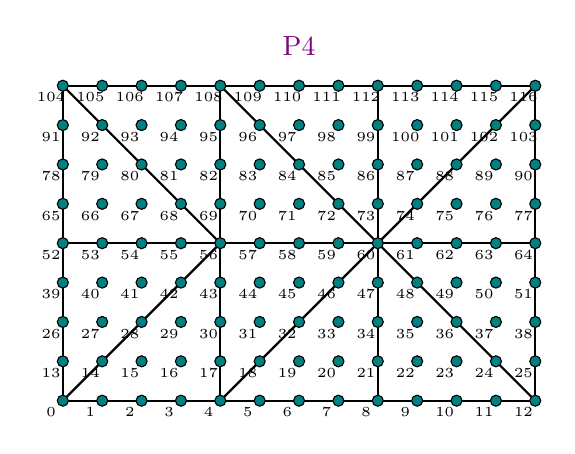
\begin{tikzpicture} 
\node[violet] at (3,4.5) {P4}; 
\draw[thick] (0,0) -- (6,0) -- (6,4) -- (0,4) -- cycle; 
\draw[thick] (0,2) -- (6,2) ; 
\draw[thick] (2,0) -- (2,4) ; 
\draw[thick] (4,0) -- (4,4) ; 
\draw[thick] (0,0) -- (2,2) -- (0,4) ; 
\draw[thick] (2,0) -- (4,2) -- (2,4) ; 
\draw[thick] (6,0) -- (4,2) -- (6,4) ; 
\draw[black,fill=teal] ( 0.000000 , 0.000000)     circle (2pt); 
\node[] at ( -0.150000, -0.150000 ) {\tiny 0 }; 
\draw[black,fill=teal] ( 0.500000 , 0.000000)     circle (2pt); 
\node[] at ( 0.350000, -0.150000 ) {\tiny 1 }; 
\draw[black,fill=teal] ( 1.000000 , 0.000000)     circle (2pt); 
\node[] at ( 0.850000, -0.150000 ) {\tiny 2 }; 
\draw[black,fill=teal] ( 1.500000 , 0.000000)     circle (2pt); 
\node[] at ( 1.350000, -0.150000 ) {\tiny 3 }; 
\draw[black,fill=teal] ( 2.000000 , 0.000000)     circle (2pt); 
\node[] at ( 1.850000, -0.150000 ) {\tiny 4 }; 
\draw[black,fill=teal] ( 2.500000 , 0.000000)     circle (2pt); 
\node[] at ( 2.350000, -0.150000 ) {\tiny 5 }; 
\draw[black,fill=teal] ( 3.000000 , 0.000000)     circle (2pt); 
\node[] at ( 2.850000, -0.150000 ) {\tiny 6 }; 
\draw[black,fill=teal] ( 3.500000 , 0.000000)     circle (2pt); 
\node[] at ( 3.350000, -0.150000 ) {\tiny 7 }; 
\draw[black,fill=teal] ( 4.000000 , 0.000000)     circle (2pt); 
\node[] at ( 3.850000, -0.150000 ) {\tiny 8 }; 
\draw[black,fill=teal] ( 4.500000 , 0.000000)     circle (2pt); 
\node[] at ( 4.350000, -0.150000 ) {\tiny 9 }; 
\draw[black,fill=teal] ( 5.000000 , 0.000000)     circle (2pt); 
\node[] at ( 4.850000, -0.150000 ) {\tiny 10 }; 
\draw[black,fill=teal] ( 5.500000 , 0.000000)     circle (2pt); 
\node[] at ( 5.350000, -0.150000 ) {\tiny 11 }; 
\draw[black,fill=teal] ( 6.000000 , 0.000000)     circle (2pt); 
\node[] at ( 5.850000, -0.150000 ) {\tiny 12 }; 
\draw[black,fill=teal] ( 0.000000 , 0.500000)     circle (2pt); 
\node[] at ( -0.150000, 0.350000 ) {\tiny 13 }; 
\draw[black,fill=teal] ( 0.500000 , 0.500000)     circle (2pt); 
\node[] at ( 0.350000, 0.350000 ) {\tiny 14 }; 
\draw[black,fill=teal] ( 1.000000 , 0.500000)     circle (2pt); 
\node[] at ( 0.850000, 0.350000 ) {\tiny 15 }; 
\draw[black,fill=teal] ( 1.500000 , 0.500000)     circle (2pt); 
\node[] at ( 1.350000, 0.350000 ) {\tiny 16 }; 
\draw[black,fill=teal] ( 2.000000 , 0.500000)     circle (2pt); 
\node[] at ( 1.850000, 0.350000 ) {\tiny 17 }; 
\draw[black,fill=teal] ( 2.500000 , 0.500000)     circle (2pt); 
\node[] at ( 2.350000, 0.350000 ) {\tiny 18 }; 
\draw[black,fill=teal] ( 3.000000 , 0.500000)     circle (2pt); 
\node[] at ( 2.850000, 0.350000 ) {\tiny 19 }; 
\draw[black,fill=teal] ( 3.500000 , 0.500000)     circle (2pt); 
\node[] at ( 3.350000, 0.350000 ) {\tiny 20 }; 
\draw[black,fill=teal] ( 4.000000 , 0.500000)     circle (2pt); 
\node[] at ( 3.850000, 0.350000 ) {\tiny 21 }; 
\draw[black,fill=teal] ( 4.500000 , 0.500000)     circle (2pt); 
\node[] at ( 4.350000, 0.350000 ) {\tiny 22 }; 
\draw[black,fill=teal] ( 5.000000 , 0.500000)     circle (2pt); 
\node[] at ( 4.850000, 0.350000 ) {\tiny 23 }; 
\draw[black,fill=teal] ( 5.500000 , 0.500000)     circle (2pt); 
\node[] at ( 5.350000, 0.350000 ) {\tiny 24 }; 
\draw[black,fill=teal] ( 6.000000 , 0.500000)     circle (2pt); 
\node[] at ( 5.850000, 0.350000 ) {\tiny 25 }; 
\draw[black,fill=teal] ( 0.000000 , 1.000000)     circle (2pt); 
\node[] at ( -0.150000, 0.850000 ) {\tiny 26 }; 
\draw[black,fill=teal] ( 0.500000 , 1.000000)     circle (2pt); 
\node[] at ( 0.350000, 0.850000 ) {\tiny 27 }; 
\draw[black,fill=teal] ( 1.000000 , 1.000000)     circle (2pt); 
\node[] at ( 0.850000, 0.850000 ) {\tiny 28 }; 
\draw[black,fill=teal] ( 1.500000 , 1.000000)     circle (2pt); 
\node[] at ( 1.350000, 0.850000 ) {\tiny 29 }; 
\draw[black,fill=teal] ( 2.000000 , 1.000000)     circle (2pt); 
\node[] at ( 1.850000, 0.850000 ) {\tiny 30 }; 
\draw[black,fill=teal] ( 2.500000 , 1.000000)     circle (2pt); 
\node[] at ( 2.350000, 0.850000 ) {\tiny 31 }; 
\draw[black,fill=teal] ( 3.000000 , 1.000000)     circle (2pt); 
\node[] at ( 2.850000, 0.850000 ) {\tiny 32 }; 
\draw[black,fill=teal] ( 3.500000 , 1.000000)     circle (2pt); 
\node[] at ( 3.350000, 0.850000 ) {\tiny 33 }; 
\draw[black,fill=teal] ( 4.000000 , 1.000000)     circle (2pt); 
\node[] at ( 3.850000, 0.850000 ) {\tiny 34 }; 
\draw[black,fill=teal] ( 4.500000 , 1.000000)     circle (2pt); 
\node[] at ( 4.350000, 0.850000 ) {\tiny 35 }; 
\draw[black,fill=teal] ( 5.000000 , 1.000000)     circle (2pt); 
\node[] at ( 4.850000, 0.850000 ) {\tiny 36 }; 
\draw[black,fill=teal] ( 5.500000 , 1.000000)     circle (2pt); 
\node[] at ( 5.350000, 0.850000 ) {\tiny 37 }; 
\draw[black,fill=teal] ( 6.000000 , 1.000000)     circle (2pt); 
\node[] at ( 5.850000, 0.850000 ) {\tiny 38 }; 
\draw[black,fill=teal] ( 0.000000 , 1.500000)     circle (2pt); 
\node[] at ( -0.150000, 1.350000 ) {\tiny 39 }; 
\draw[black,fill=teal] ( 0.500000 , 1.500000)     circle (2pt); 
\node[] at ( 0.350000, 1.350000 ) {\tiny 40 }; 
\draw[black,fill=teal] ( 1.000000 , 1.500000)     circle (2pt); 
\node[] at ( 0.850000, 1.350000 ) {\tiny 41 }; 
\draw[black,fill=teal] ( 1.500000 , 1.500000)     circle (2pt); 
\node[] at ( 1.350000, 1.350000 ) {\tiny 42 }; 
\draw[black,fill=teal] ( 2.000000 , 1.500000)     circle (2pt); 
\node[] at ( 1.850000, 1.350000 ) {\tiny 43 }; 
\draw[black,fill=teal] ( 2.500000 , 1.500000)     circle (2pt); 
\node[] at ( 2.350000, 1.350000 ) {\tiny 44 }; 
\draw[black,fill=teal] ( 3.000000 , 1.500000)     circle (2pt); 
\node[] at ( 2.850000, 1.350000 ) {\tiny 45 }; 
\draw[black,fill=teal] ( 3.500000 , 1.500000)     circle (2pt); 
\node[] at ( 3.350000, 1.350000 ) {\tiny 46 }; 
\draw[black,fill=teal] ( 4.000000 , 1.500000)     circle (2pt); 
\node[] at ( 3.850000, 1.350000 ) {\tiny 47 }; 
\draw[black,fill=teal] ( 4.500000 , 1.500000)     circle (2pt); 
\node[] at ( 4.350000, 1.350000 ) {\tiny 48 }; 
\draw[black,fill=teal] ( 5.000000 , 1.500000)     circle (2pt); 
\node[] at ( 4.850000, 1.350000 ) {\tiny 49 }; 
\draw[black,fill=teal] ( 5.500000 , 1.500000)     circle (2pt); 
\node[] at ( 5.350000, 1.350000 ) {\tiny 50 }; 
\draw[black,fill=teal] ( 6.000000 , 1.500000)     circle (2pt); 
\node[] at ( 5.850000, 1.350000 ) {\tiny 51 }; 
\draw[black,fill=teal] ( 0.000000 , 2.000000)     circle (2pt); 
\node[] at ( -0.150000, 1.850000 ) {\tiny 52 }; 
\draw[black,fill=teal] ( 0.500000 , 2.000000)     circle (2pt); 
\node[] at ( 0.350000, 1.850000 ) {\tiny 53 }; 
\draw[black,fill=teal] ( 1.000000 , 2.000000)     circle (2pt); 
\node[] at ( 0.850000, 1.850000 ) {\tiny 54 }; 
\draw[black,fill=teal] ( 1.500000 , 2.000000)     circle (2pt); 
\node[] at ( 1.350000, 1.850000 ) {\tiny 55 }; 
\draw[black,fill=teal] ( 2.000000 , 2.000000)     circle (2pt); 
\node[] at ( 1.850000, 1.850000 ) {\tiny 56 }; 
\draw[black,fill=teal] ( 2.500000 , 2.000000)     circle (2pt); 
\node[] at ( 2.350000, 1.850000 ) {\tiny 57 }; 
\draw[black,fill=teal] ( 3.000000 , 2.000000)     circle (2pt); 
\node[] at ( 2.850000, 1.850000 ) {\tiny 58 }; 
\draw[black,fill=teal] ( 3.500000 , 2.000000)     circle (2pt); 
\node[] at ( 3.350000, 1.850000 ) {\tiny 59 }; 
\draw[black,fill=teal] ( 4.000000 , 2.000000)     circle (2pt); 
\node[] at ( 3.850000, 1.850000 ) {\tiny 60 }; 
\draw[black,fill=teal] ( 4.500000 , 2.000000)     circle (2pt); 
\node[] at ( 4.350000, 1.850000 ) {\tiny 61 }; 
\draw[black,fill=teal] ( 5.000000 , 2.000000)     circle (2pt); 
\node[] at ( 4.850000, 1.850000 ) {\tiny 62 }; 
\draw[black,fill=teal] ( 5.500000 , 2.000000)     circle (2pt); 
\node[] at ( 5.350000, 1.850000 ) {\tiny 63 }; 
\draw[black,fill=teal] ( 6.000000 , 2.000000)     circle (2pt); 
\node[] at ( 5.850000, 1.850000 ) {\tiny 64 }; 
\draw[black,fill=teal] ( 0.000000 , 2.500000)     circle (2pt); 
\node[] at ( -0.150000, 2.350000 ) {\tiny 65 }; 
\draw[black,fill=teal] ( 0.500000 , 2.500000)     circle (2pt); 
\node[] at ( 0.350000, 2.350000 ) {\tiny 66 }; 
\draw[black,fill=teal] ( 1.000000 , 2.500000)     circle (2pt); 
\node[] at ( 0.850000, 2.350000 ) {\tiny 67 }; 
\draw[black,fill=teal] ( 1.500000 , 2.500000)     circle (2pt); 
\node[] at ( 1.350000, 2.350000 ) {\tiny 68 }; 
\draw[black,fill=teal] ( 2.000000 , 2.500000)     circle (2pt); 
\node[] at ( 1.850000, 2.350000 ) {\tiny 69 }; 
\draw[black,fill=teal] ( 2.500000 , 2.500000)     circle (2pt); 
\node[] at ( 2.350000, 2.350000 ) {\tiny 70 }; 
\draw[black,fill=teal] ( 3.000000 , 2.500000)     circle (2pt); 
\node[] at ( 2.850000, 2.350000 ) {\tiny 71 }; 
\draw[black,fill=teal] ( 3.500000 , 2.500000)     circle (2pt); 
\node[] at ( 3.350000, 2.350000 ) {\tiny 72 }; 
\draw[black,fill=teal] ( 4.000000 , 2.500000)     circle (2pt); 
\node[] at ( 3.850000, 2.350000 ) {\tiny 73 }; 
\draw[black,fill=teal] ( 4.500000 , 2.500000)     circle (2pt); 
\node[] at ( 4.350000, 2.350000 ) {\tiny 74 }; 
\draw[black,fill=teal] ( 5.000000 , 2.500000)     circle (2pt); 
\node[] at ( 4.850000, 2.350000 ) {\tiny 75 }; 
\draw[black,fill=teal] ( 5.500000 , 2.500000)     circle (2pt); 
\node[] at ( 5.350000, 2.350000 ) {\tiny 76 }; 
\draw[black,fill=teal] ( 6.000000 , 2.500000)     circle (2pt); 
\node[] at ( 5.850000, 2.350000 ) {\tiny 77 }; 
\draw[black,fill=teal] ( 0.000000 , 3.000000)     circle (2pt); 
\node[] at ( -0.150000, 2.850000 ) {\tiny 78 }; 
\draw[black,fill=teal] ( 0.500000 , 3.000000)     circle (2pt); 
\node[] at ( 0.350000, 2.850000 ) {\tiny 79 }; 
\draw[black,fill=teal] ( 1.000000 , 3.000000)     circle (2pt); 
\node[] at ( 0.850000, 2.850000 ) {\tiny 80 }; 
\draw[black,fill=teal] ( 1.500000 , 3.000000)     circle (2pt); 
\node[] at ( 1.350000, 2.850000 ) {\tiny 81 }; 
\draw[black,fill=teal] ( 2.000000 , 3.000000)     circle (2pt); 
\node[] at ( 1.850000, 2.850000 ) {\tiny 82 }; 
\draw[black,fill=teal] ( 2.500000 , 3.000000)     circle (2pt); 
\node[] at ( 2.350000, 2.850000 ) {\tiny 83 }; 
\draw[black,fill=teal] ( 3.000000 , 3.000000)     circle (2pt); 
\node[] at ( 2.850000, 2.850000 ) {\tiny 84 }; 
\draw[black,fill=teal] ( 3.500000 , 3.000000)     circle (2pt); 
\node[] at ( 3.350000, 2.850000 ) {\tiny 85 }; 
\draw[black,fill=teal] ( 4.000000 , 3.000000)     circle (2pt); 
\node[] at ( 3.850000, 2.850000 ) {\tiny 86 }; 
\draw[black,fill=teal] ( 4.500000 , 3.000000)     circle (2pt); 
\node[] at ( 4.350000, 2.850000 ) {\tiny 87 }; 
\draw[black,fill=teal] ( 5.000000 , 3.000000)     circle (2pt); 
\node[] at ( 4.850000, 2.850000 ) {\tiny 88 }; 
\draw[black,fill=teal] ( 5.500000 , 3.000000)     circle (2pt); 
\node[] at ( 5.350000, 2.850000 ) {\tiny 89 }; 
\draw[black,fill=teal] ( 6.000000 , 3.000000)     circle (2pt); 
\node[] at ( 5.850000, 2.850000 ) {\tiny 90 }; 
\draw[black,fill=teal] ( 0.000000 , 3.500000)     circle (2pt); 
\node[] at ( -0.150000, 3.350000 ) {\tiny 91 }; 
\draw[black,fill=teal] ( 0.500000 , 3.500000)     circle (2pt); 
\node[] at ( 0.350000, 3.350000 ) {\tiny 92 }; 
\draw[black,fill=teal] ( 1.000000 , 3.500000)     circle (2pt); 
\node[] at ( 0.850000, 3.350000 ) {\tiny 93 }; 
\draw[black,fill=teal] ( 1.500000 , 3.500000)     circle (2pt); 
\node[] at ( 1.350000, 3.350000 ) {\tiny 94 }; 
\draw[black,fill=teal] ( 2.000000 , 3.500000)     circle (2pt); 
\node[] at ( 1.850000, 3.350000 ) {\tiny 95 }; 
\draw[black,fill=teal] ( 2.500000 , 3.500000)     circle (2pt); 
\node[] at ( 2.350000, 3.350000 ) {\tiny 96 }; 
\draw[black,fill=teal] ( 3.000000 , 3.500000)     circle (2pt); 
\node[] at ( 2.850000, 3.350000 ) {\tiny 97 }; 
\draw[black,fill=teal] ( 3.500000 , 3.500000)     circle (2pt); 
\node[] at ( 3.350000, 3.350000 ) {\tiny 98 }; 
\draw[black,fill=teal] ( 4.000000 , 3.500000)     circle (2pt); 
\node[] at ( 3.850000, 3.350000 ) {\tiny 99 }; 
\draw[black,fill=teal] ( 4.500000 , 3.500000)     circle (2pt); 
\node[] at ( 4.350000, 3.350000 ) {\tiny 100 }; 
\draw[black,fill=teal] ( 5.000000 , 3.500000)     circle (2pt); 
\node[] at ( 4.850000, 3.350000 ) {\tiny 101 }; 
\draw[black,fill=teal] ( 5.500000 , 3.500000)     circle (2pt); 
\node[] at ( 5.350000, 3.350000 ) {\tiny 102 }; 
\draw[black,fill=teal] ( 6.000000 , 3.500000)     circle (2pt); 
\node[] at ( 5.850000, 3.350000 ) {\tiny 103 }; 
\draw[black,fill=teal] ( 0.000000 , 4.000000)     circle (2pt); 
\node[] at ( -0.150000, 3.850000 ) {\tiny 104 }; 
\draw[black,fill=teal] ( 0.500000 , 4.000000)     circle (2pt); 
\node[] at ( 0.350000, 3.850000 ) {\tiny 105 }; 
\draw[black,fill=teal] ( 1.000000 , 4.000000)     circle (2pt); 
\node[] at ( 0.850000, 3.850000 ) {\tiny 106 }; 
\draw[black,fill=teal] ( 1.500000 , 4.000000)     circle (2pt); 
\node[] at ( 1.350000, 3.850000 ) {\tiny 107 }; 
\draw[black,fill=teal] ( 2.000000 , 4.000000)     circle (2pt); 
\node[] at ( 1.850000, 3.850000 ) {\tiny 108 }; 
\draw[black,fill=teal] ( 2.500000 , 4.000000)     circle (2pt); 
\node[] at ( 2.350000, 3.850000 ) {\tiny 109 }; 
\draw[black,fill=teal] ( 3.000000 , 4.000000)     circle (2pt); 
\node[] at ( 2.850000, 3.850000 ) {\tiny 110 }; 
\draw[black,fill=teal] ( 3.500000 , 4.000000)     circle (2pt); 
\node[] at ( 3.350000, 3.850000 ) {\tiny 111 }; 
\draw[black,fill=teal] ( 4.000000 , 4.000000)     circle (2pt); 
\node[] at ( 3.850000, 3.850000 ) {\tiny 112 }; 
\draw[black,fill=teal] ( 4.500000 , 4.000000)     circle (2pt); 
\node[] at ( 4.350000, 3.850000 ) {\tiny 113 }; 
\draw[black,fill=teal] ( 5.000000 , 4.000000)     circle (2pt); 
\node[] at ( 4.850000, 3.850000 ) {\tiny 114 }; 
\draw[black,fill=teal] ( 5.500000 , 4.000000)     circle (2pt); 
\node[] at ( 5.350000, 3.850000 ) {\tiny 115 }; 
\draw[black,fill=teal] ( 6.000000 , 4.000000)     circle (2pt); 
\node[] at ( 5.850000, 3.850000 ) {\tiny 116 }; 
\end{tikzpicture} 
\end{center} 


\begin{tiny}
\verbatiminput{python_codes/fieldstone_120/spaces/iconV_elt1_P4.ascii}
\end{tiny}
\end{multicols}




\newpage
%------------------
\begin{multicols}{2}
\begin{center} 
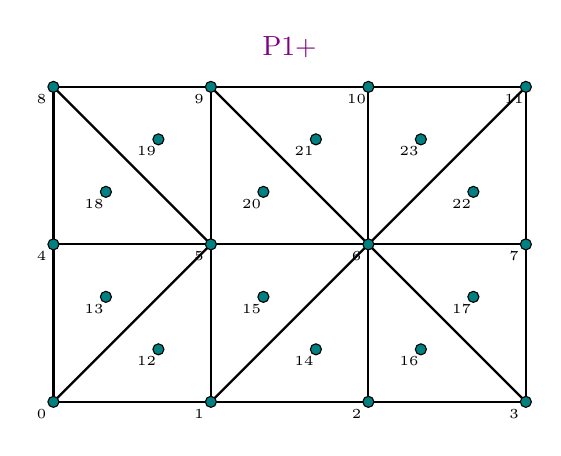
\begin{tikzpicture} 
\node[violet] at (3,4.5) {P1+}; 
\draw[thick] (0,0) -- (6,0) -- (6,4) -- (0,4) -- cycle; 
\draw[thick] (0,2) -- (6,2) ; 
\draw[thick] (2,0) -- (2,4) ; 
\draw[thick] (4,0) -- (4,4) ; 
\draw[thick] (0,0) -- (2,2) -- (0,4) ; 
\draw[thick] (2,0) -- (4,2) -- (2,4) ; 
\draw[thick] (6,0) -- (4,2) -- (6,4) ; 
\draw[black,fill=teal] ( 0.000000 , 0.000000)     circle (2pt); 
\node[] at ( -0.150000, -0.150000 ) {\tiny 0 }; 
\draw[black,fill=teal] ( 2.000000 , 0.000000)     circle (2pt); 
\node[] at ( 1.850000, -0.150000 ) {\tiny 1 }; 
\draw[black,fill=teal] ( 4.000000 , 0.000000)     circle (2pt); 
\node[] at ( 3.850000, -0.150000 ) {\tiny 2 }; 
\draw[black,fill=teal] ( 6.000000 , 0.000000)     circle (2pt); 
\node[] at ( 5.850000, -0.150000 ) {\tiny 3 }; 
\draw[black,fill=teal] ( 0.000000 , 2.000000)     circle (2pt); 
\node[] at ( -0.150000, 1.850000 ) {\tiny 4 }; 
\draw[black,fill=teal] ( 2.000000 , 2.000000)     circle (2pt); 
\node[] at ( 1.850000, 1.850000 ) {\tiny 5 }; 
\draw[black,fill=teal] ( 4.000000 , 2.000000)     circle (2pt); 
\node[] at ( 3.850000, 1.850000 ) {\tiny 6 }; 
\draw[black,fill=teal] ( 6.000000 , 2.000000)     circle (2pt); 
\node[] at ( 5.850000, 1.850000 ) {\tiny 7 }; 
\draw[black,fill=teal] ( 0.000000 , 4.000000)     circle (2pt); 
\node[] at ( -0.150000, 3.850000 ) {\tiny 8 }; 
\draw[black,fill=teal] ( 2.000000 , 4.000000)     circle (2pt); 
\node[] at ( 1.850000, 3.850000 ) {\tiny 9 }; 
\draw[black,fill=teal] ( 4.000000 , 4.000000)     circle (2pt); 
\node[] at ( 3.850000, 3.850000 ) {\tiny 10 }; 
\draw[black,fill=teal] ( 6.000000 , 4.000000)     circle (2pt); 
\node[] at ( 5.850000, 3.850000 ) {\tiny 11 }; 
\draw[black,fill=teal] ( 1.333333 , 0.666667)     circle (2pt); 
\node[] at ( 1.183333, 0.516667 ) {\tiny 12 }; 
\draw[black,fill=teal] ( 0.666667 , 1.333333)     circle (2pt); 
\node[] at ( 0.516667, 1.183333 ) {\tiny 13 }; 
\draw[black,fill=teal] ( 3.333333 , 0.666667)     circle (2pt); 
\node[] at ( 3.183333, 0.516667 ) {\tiny 14 }; 
\draw[black,fill=teal] ( 2.666667 , 1.333333)     circle (2pt); 
\node[] at ( 2.516667, 1.183333 ) {\tiny 15 }; 
\draw[black,fill=teal] ( 4.666667 , 0.666667)     circle (2pt); 
\node[] at ( 4.516667, 0.516667 ) {\tiny 16 }; 
\draw[black,fill=teal] ( 5.333333 , 1.333333)     circle (2pt); 
\node[] at ( 5.183333, 1.183333 ) {\tiny 17 }; 
\draw[black,fill=teal] ( 0.666667 , 2.666667)     circle (2pt); 
\node[] at ( 0.516667, 2.516667 ) {\tiny 18 }; 
\draw[black,fill=teal] ( 1.333333 , 3.333333)     circle (2pt); 
\node[] at ( 1.183333, 3.183333 ) {\tiny 19 }; 
\draw[black,fill=teal] ( 2.666667 , 2.666667)     circle (2pt); 
\node[] at ( 2.516667, 2.516667 ) {\tiny 20 }; 
\draw[black,fill=teal] ( 3.333333 , 3.333333)     circle (2pt); 
\node[] at ( 3.183333, 3.183333 ) {\tiny 21 }; 
\draw[black,fill=teal] ( 5.333333 , 2.666667)     circle (2pt); 
\node[] at ( 5.183333, 2.516667 ) {\tiny 22 }; 
\draw[black,fill=teal] ( 4.666667 , 3.333333)     circle (2pt); 
\node[] at ( 4.516667, 3.183333 ) {\tiny 23 }; 
\end{tikzpicture} 
\end{center} 


\begin{tiny}
\verbatiminput{python_codes/fieldstone_120/spaces/iconV_elt1_P1+.ascii}
\end{tiny}
\end{multicols}

%------------------
\begin{multicols}{2}
\begin{center} 
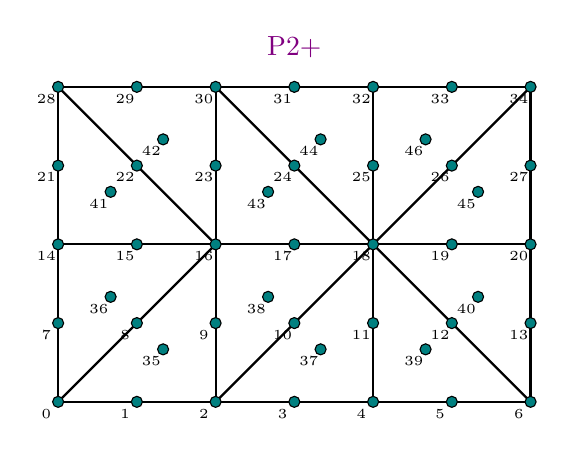
\begin{tikzpicture} 
\node[violet] at (3,4.5) {P2+}; 
\draw[thick] (0,0) -- (6,0) -- (6,4) -- (0,4) -- cycle; 
\draw[thick] (0,2) -- (6,2) ; 
\draw[thick] (2,0) -- (2,4) ; 
\draw[thick] (4,0) -- (4,4) ; 
\draw[thick] (0,0) -- (2,2) -- (0,4) ; 
\draw[thick] (2,0) -- (4,2) -- (2,4) ; 
\draw[thick] (6,0) -- (4,2) -- (6,4) ; 
\draw[black,fill=teal] ( 0.000000 , 0.000000)     circle (2pt); 
\node[] at ( -0.150000, -0.150000 ) {\tiny 0 }; 
\draw[black,fill=teal] ( 1.000000 , 0.000000)     circle (2pt); 
\node[] at ( 0.850000, -0.150000 ) {\tiny 1 }; 
\draw[black,fill=teal] ( 2.000000 , 0.000000)     circle (2pt); 
\node[] at ( 1.850000, -0.150000 ) {\tiny 2 }; 
\draw[black,fill=teal] ( 3.000000 , 0.000000)     circle (2pt); 
\node[] at ( 2.850000, -0.150000 ) {\tiny 3 }; 
\draw[black,fill=teal] ( 4.000000 , 0.000000)     circle (2pt); 
\node[] at ( 3.850000, -0.150000 ) {\tiny 4 }; 
\draw[black,fill=teal] ( 5.000000 , 0.000000)     circle (2pt); 
\node[] at ( 4.850000, -0.150000 ) {\tiny 5 }; 
\draw[black,fill=teal] ( 6.000000 , 0.000000)     circle (2pt); 
\node[] at ( 5.850000, -0.150000 ) {\tiny 6 }; 
\draw[black,fill=teal] ( 0.000000 , 1.000000)     circle (2pt); 
\node[] at ( -0.150000, 0.850000 ) {\tiny 7 }; 
\draw[black,fill=teal] ( 1.000000 , 1.000000)     circle (2pt); 
\node[] at ( 0.850000, 0.850000 ) {\tiny 8 }; 
\draw[black,fill=teal] ( 2.000000 , 1.000000)     circle (2pt); 
\node[] at ( 1.850000, 0.850000 ) {\tiny 9 }; 
\draw[black,fill=teal] ( 3.000000 , 1.000000)     circle (2pt); 
\node[] at ( 2.850000, 0.850000 ) {\tiny 10 }; 
\draw[black,fill=teal] ( 4.000000 , 1.000000)     circle (2pt); 
\node[] at ( 3.850000, 0.850000 ) {\tiny 11 }; 
\draw[black,fill=teal] ( 5.000000 , 1.000000)     circle (2pt); 
\node[] at ( 4.850000, 0.850000 ) {\tiny 12 }; 
\draw[black,fill=teal] ( 6.000000 , 1.000000)     circle (2pt); 
\node[] at ( 5.850000, 0.850000 ) {\tiny 13 }; 
\draw[black,fill=teal] ( 0.000000 , 2.000000)     circle (2pt); 
\node[] at ( -0.150000, 1.850000 ) {\tiny 14 }; 
\draw[black,fill=teal] ( 1.000000 , 2.000000)     circle (2pt); 
\node[] at ( 0.850000, 1.850000 ) {\tiny 15 }; 
\draw[black,fill=teal] ( 2.000000 , 2.000000)     circle (2pt); 
\node[] at ( 1.850000, 1.850000 ) {\tiny 16 }; 
\draw[black,fill=teal] ( 3.000000 , 2.000000)     circle (2pt); 
\node[] at ( 2.850000, 1.850000 ) {\tiny 17 }; 
\draw[black,fill=teal] ( 4.000000 , 2.000000)     circle (2pt); 
\node[] at ( 3.850000, 1.850000 ) {\tiny 18 }; 
\draw[black,fill=teal] ( 5.000000 , 2.000000)     circle (2pt); 
\node[] at ( 4.850000, 1.850000 ) {\tiny 19 }; 
\draw[black,fill=teal] ( 6.000000 , 2.000000)     circle (2pt); 
\node[] at ( 5.850000, 1.850000 ) {\tiny 20 }; 
\draw[black,fill=teal] ( 0.000000 , 3.000000)     circle (2pt); 
\node[] at ( -0.150000, 2.850000 ) {\tiny 21 }; 
\draw[black,fill=teal] ( 1.000000 , 3.000000)     circle (2pt); 
\node[] at ( 0.850000, 2.850000 ) {\tiny 22 }; 
\draw[black,fill=teal] ( 2.000000 , 3.000000)     circle (2pt); 
\node[] at ( 1.850000, 2.850000 ) {\tiny 23 }; 
\draw[black,fill=teal] ( 3.000000 , 3.000000)     circle (2pt); 
\node[] at ( 2.850000, 2.850000 ) {\tiny 24 }; 
\draw[black,fill=teal] ( 4.000000 , 3.000000)     circle (2pt); 
\node[] at ( 3.850000, 2.850000 ) {\tiny 25 }; 
\draw[black,fill=teal] ( 5.000000 , 3.000000)     circle (2pt); 
\node[] at ( 4.850000, 2.850000 ) {\tiny 26 }; 
\draw[black,fill=teal] ( 6.000000 , 3.000000)     circle (2pt); 
\node[] at ( 5.850000, 2.850000 ) {\tiny 27 }; 
\draw[black,fill=teal] ( 0.000000 , 4.000000)     circle (2pt); 
\node[] at ( -0.150000, 3.850000 ) {\tiny 28 }; 
\draw[black,fill=teal] ( 1.000000 , 4.000000)     circle (2pt); 
\node[] at ( 0.850000, 3.850000 ) {\tiny 29 }; 
\draw[black,fill=teal] ( 2.000000 , 4.000000)     circle (2pt); 
\node[] at ( 1.850000, 3.850000 ) {\tiny 30 }; 
\draw[black,fill=teal] ( 3.000000 , 4.000000)     circle (2pt); 
\node[] at ( 2.850000, 3.850000 ) {\tiny 31 }; 
\draw[black,fill=teal] ( 4.000000 , 4.000000)     circle (2pt); 
\node[] at ( 3.850000, 3.850000 ) {\tiny 32 }; 
\draw[black,fill=teal] ( 5.000000 , 4.000000)     circle (2pt); 
\node[] at ( 4.850000, 3.850000 ) {\tiny 33 }; 
\draw[black,fill=teal] ( 6.000000 , 4.000000)     circle (2pt); 
\node[] at ( 5.850000, 3.850000 ) {\tiny 34 }; 
\draw[black,fill=teal] ( 1.333333 , 0.666667)     circle (2pt); 
\node[] at ( 1.183333, 0.516667 ) {\tiny 35 }; 
\draw[black,fill=teal] ( 0.666667 , 1.333333)     circle (2pt); 
\node[] at ( 0.516667, 1.183333 ) {\tiny 36 }; 
\draw[black,fill=teal] ( 3.333333 , 0.666667)     circle (2pt); 
\node[] at ( 3.183333, 0.516667 ) {\tiny 37 }; 
\draw[black,fill=teal] ( 2.666667 , 1.333333)     circle (2pt); 
\node[] at ( 2.516667, 1.183333 ) {\tiny 38 }; 
\draw[black,fill=teal] ( 4.666667 , 0.666667)     circle (2pt); 
\node[] at ( 4.516667, 0.516667 ) {\tiny 39 }; 
\draw[black,fill=teal] ( 5.333333 , 1.333333)     circle (2pt); 
\node[] at ( 5.183333, 1.183333 ) {\tiny 40 }; 
\draw[black,fill=teal] ( 0.666667 , 2.666667)     circle (2pt); 
\node[] at ( 0.516667, 2.516667 ) {\tiny 41 }; 
\draw[black,fill=teal] ( 1.333333 , 3.333333)     circle (2pt); 
\node[] at ( 1.183333, 3.183333 ) {\tiny 42 }; 
\draw[black,fill=teal] ( 2.666667 , 2.666667)     circle (2pt); 
\node[] at ( 2.516667, 2.516667 ) {\tiny 43 }; 
\draw[black,fill=teal] ( 3.333333 , 3.333333)     circle (2pt); 
\node[] at ( 3.183333, 3.183333 ) {\tiny 44 }; 
\draw[black,fill=teal] ( 5.333333 , 2.666667)     circle (2pt); 
\node[] at ( 5.183333, 2.516667 ) {\tiny 45 }; 
\draw[black,fill=teal] ( 4.666667 , 3.333333)     circle (2pt); 
\node[] at ( 4.516667, 3.183333 ) {\tiny 46 }; 
\end{tikzpicture} 
\end{center} 


\begin{tiny}
\verbatiminput{python_codes/fieldstone_120/spaces/iconV_elt1_P2+.ascii}
\end{tiny}
\end{multicols}

%------------------
\begin{multicols}{2}
\begin{center} 
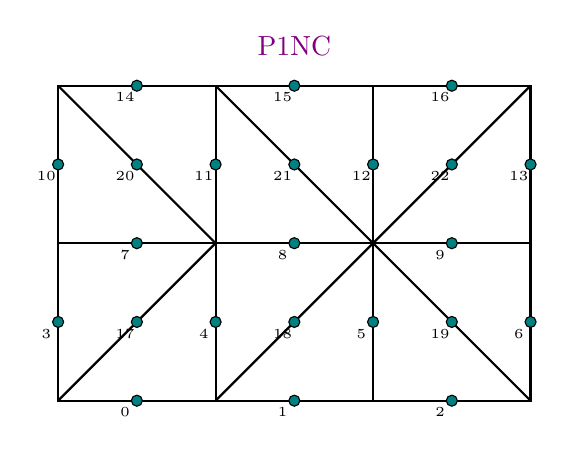
\begin{tikzpicture} 
\node[violet] at (3,4.5) {P1NC}; 
\draw[thick] (0,0) -- (6,0) -- (6,4) -- (0,4) -- cycle; 
\draw[thick] (0,2) -- (6,2) ; 
\draw[thick] (2,0) -- (2,4) ; 
\draw[thick] (4,0) -- (4,4) ; 
\draw[thick] (0,0) -- (2,2) -- (0,4) ; 
\draw[thick] (2,0) -- (4,2) -- (2,4) ; 
\draw[thick] (6,0) -- (4,2) -- (6,4) ; 
\draw[black,fill=teal] ( 1.000000 , 0.000000)     circle (2pt); 
\node[] at ( 0.850000, -0.150000 ) {\tiny 0 }; 
\draw[black,fill=teal] ( 3.000000 , 0.000000)     circle (2pt); 
\node[] at ( 2.850000, -0.150000 ) {\tiny 1 }; 
\draw[black,fill=teal] ( 5.000000 , 0.000000)     circle (2pt); 
\node[] at ( 4.850000, -0.150000 ) {\tiny 2 }; 
\draw[black,fill=teal] ( 0.000000 , 1.000000)     circle (2pt); 
\node[] at ( -0.150000, 0.850000 ) {\tiny 3 }; 
\draw[black,fill=teal] ( 2.000000 , 1.000000)     circle (2pt); 
\node[] at ( 1.850000, 0.850000 ) {\tiny 4 }; 
\draw[black,fill=teal] ( 4.000000 , 1.000000)     circle (2pt); 
\node[] at ( 3.850000, 0.850000 ) {\tiny 5 }; 
\draw[black,fill=teal] ( 6.000000 , 1.000000)     circle (2pt); 
\node[] at ( 5.850000, 0.850000 ) {\tiny 6 }; 
\draw[black,fill=teal] ( 1.000000 , 2.000000)     circle (2pt); 
\node[] at ( 0.850000, 1.850000 ) {\tiny 7 }; 
\draw[black,fill=teal] ( 3.000000 , 2.000000)     circle (2pt); 
\node[] at ( 2.850000, 1.850000 ) {\tiny 8 }; 
\draw[black,fill=teal] ( 5.000000 , 2.000000)     circle (2pt); 
\node[] at ( 4.850000, 1.850000 ) {\tiny 9 }; 
\draw[black,fill=teal] ( 0.000000 , 3.000000)     circle (2pt); 
\node[] at ( -0.150000, 2.850000 ) {\tiny 10 }; 
\draw[black,fill=teal] ( 2.000000 , 3.000000)     circle (2pt); 
\node[] at ( 1.850000, 2.850000 ) {\tiny 11 }; 
\draw[black,fill=teal] ( 4.000000 , 3.000000)     circle (2pt); 
\node[] at ( 3.850000, 2.850000 ) {\tiny 12 }; 
\draw[black,fill=teal] ( 6.000000 , 3.000000)     circle (2pt); 
\node[] at ( 5.850000, 2.850000 ) {\tiny 13 }; 
\draw[black,fill=teal] ( 1.000000 , 4.000000)     circle (2pt); 
\node[] at ( 0.850000, 3.850000 ) {\tiny 14 }; 
\draw[black,fill=teal] ( 3.000000 , 4.000000)     circle (2pt); 
\node[] at ( 2.850000, 3.850000 ) {\tiny 15 }; 
\draw[black,fill=teal] ( 5.000000 , 4.000000)     circle (2pt); 
\node[] at ( 4.850000, 3.850000 ) {\tiny 16 }; 
\draw[black,fill=teal] ( 1.000000 , 1.000000)     circle (2pt); 
\node[] at ( 0.850000, 0.850000 ) {\tiny 17 }; 
\draw[black,fill=teal] ( 3.000000 , 1.000000)     circle (2pt); 
\node[] at ( 2.850000, 0.850000 ) {\tiny 18 }; 
\draw[black,fill=teal] ( 5.000000 , 1.000000)     circle (2pt); 
\node[] at ( 4.850000, 0.850000 ) {\tiny 19 }; 
\draw[black,fill=teal] ( 1.000000 , 3.000000)     circle (2pt); 
\node[] at ( 0.850000, 2.850000 ) {\tiny 20 }; 
\draw[black,fill=teal] ( 3.000000 , 3.000000)     circle (2pt); 
\node[] at ( 2.850000, 2.850000 ) {\tiny 21 }; 
\draw[black,fill=teal] ( 5.000000 , 3.000000)     circle (2pt); 
\node[] at ( 4.850000, 2.850000 ) {\tiny 22 }; 
\end{tikzpicture} 
\end{center} 


\begin{tiny}
\verbatiminput{python_codes/fieldstone_120/spaces/iconV_elt1_P1NC.ascii}
\end{tiny}
\end{multicols}

\newpage
%------------------
\begin{multicols}{2}
\begin{center} 
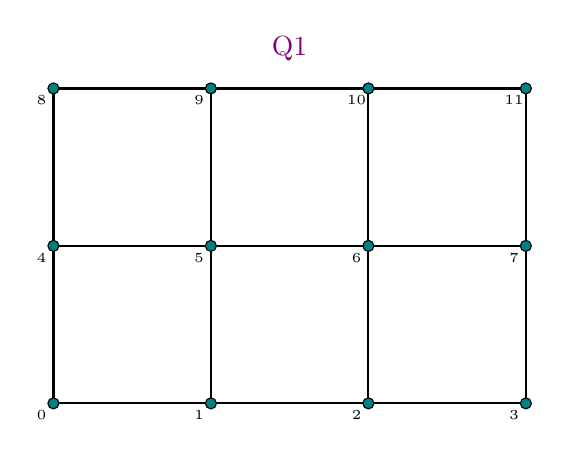
\begin{tikzpicture} 
\node[violet] at (3,4.5) {Q1}; 
\draw[thick] (0,0) -- (6,0) -- (6,4) -- (0,4) -- cycle; 
\draw[thick] (0,2) -- (6,2) ; 
\draw[thick] (2,0) -- (2,4) ; 
\draw[thick] (4,0) -- (4,4) ; 
\draw[black,fill=teal] ( 0.000000 , 0.000000)     circle (2pt); 
\node[] at ( -0.150000, -0.150000 ) {\tiny 0 }; 
\draw[black,fill=teal] ( 2.000000 , 0.000000)     circle (2pt); 
\node[] at ( 1.850000, -0.150000 ) {\tiny 1 }; 
\draw[black,fill=teal] ( 4.000000 , 0.000000)     circle (2pt); 
\node[] at ( 3.850000, -0.150000 ) {\tiny 2 }; 
\draw[black,fill=teal] ( 6.000000 , 0.000000)     circle (2pt); 
\node[] at ( 5.850000, -0.150000 ) {\tiny 3 }; 
\draw[black,fill=teal] ( 0.000000 , 2.000000)     circle (2pt); 
\node[] at ( -0.150000, 1.850000 ) {\tiny 4 }; 
\draw[black,fill=teal] ( 2.000000 , 2.000000)     circle (2pt); 
\node[] at ( 1.850000, 1.850000 ) {\tiny 5 }; 
\draw[black,fill=teal] ( 4.000000 , 2.000000)     circle (2pt); 
\node[] at ( 3.850000, 1.850000 ) {\tiny 6 }; 
\draw[black,fill=teal] ( 6.000000 , 2.000000)     circle (2pt); 
\node[] at ( 5.850000, 1.850000 ) {\tiny 7 }; 
\draw[black,fill=teal] ( 0.000000 , 4.000000)     circle (2pt); 
\node[] at ( -0.150000, 3.850000 ) {\tiny 8 }; 
\draw[black,fill=teal] ( 2.000000 , 4.000000)     circle (2pt); 
\node[] at ( 1.850000, 3.850000 ) {\tiny 9 }; 
\draw[black,fill=teal] ( 4.000000 , 4.000000)     circle (2pt); 
\node[] at ( 3.850000, 3.850000 ) {\tiny 10 }; 
\draw[black,fill=teal] ( 6.000000 , 4.000000)     circle (2pt); 
\node[] at ( 5.850000, 3.850000 ) {\tiny 11 }; 
\end{tikzpicture} 
\end{center} 


\begin{tiny}
\verbatiminput{python_codes/fieldstone_120/spaces/iconV_elt1_Q1.ascii}
\end{tiny}
\end{multicols}

%------------------
\begin{multicols}{2}
\begin{center} 
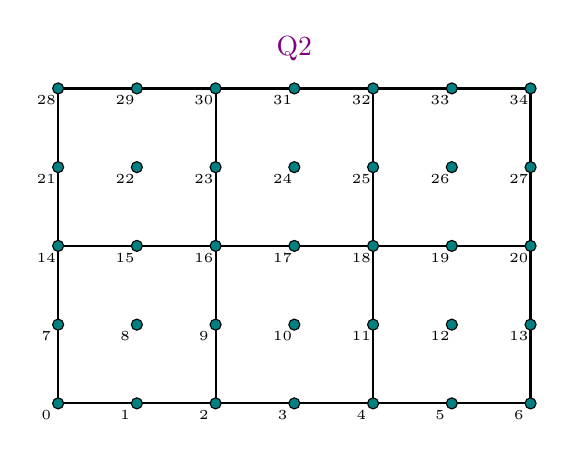
\begin{tikzpicture} 
\node[violet] at (3,4.5) {Q2}; 
\draw[thick] (0,0) -- (6,0) -- (6,4) -- (0,4) -- cycle; 
\draw[thick] (0,2) -- (6,2) ; 
\draw[thick] (2,0) -- (2,4) ; 
\draw[thick] (4,0) -- (4,4) ; 
\draw[black,fill=teal] ( 0.000000 , 0.000000)     circle (2pt); 
\node[] at ( -0.150000, -0.150000 ) {\tiny 0 }; 
\draw[black,fill=teal] ( 1.000000 , 0.000000)     circle (2pt); 
\node[] at ( 0.850000, -0.150000 ) {\tiny 1 }; 
\draw[black,fill=teal] ( 2.000000 , 0.000000)     circle (2pt); 
\node[] at ( 1.850000, -0.150000 ) {\tiny 2 }; 
\draw[black,fill=teal] ( 3.000000 , 0.000000)     circle (2pt); 
\node[] at ( 2.850000, -0.150000 ) {\tiny 3 }; 
\draw[black,fill=teal] ( 4.000000 , 0.000000)     circle (2pt); 
\node[] at ( 3.850000, -0.150000 ) {\tiny 4 }; 
\draw[black,fill=teal] ( 5.000000 , 0.000000)     circle (2pt); 
\node[] at ( 4.850000, -0.150000 ) {\tiny 5 }; 
\draw[black,fill=teal] ( 6.000000 , 0.000000)     circle (2pt); 
\node[] at ( 5.850000, -0.150000 ) {\tiny 6 }; 
\draw[black,fill=teal] ( 0.000000 , 1.000000)     circle (2pt); 
\node[] at ( -0.150000, 0.850000 ) {\tiny 7 }; 
\draw[black,fill=teal] ( 1.000000 , 1.000000)     circle (2pt); 
\node[] at ( 0.850000, 0.850000 ) {\tiny 8 }; 
\draw[black,fill=teal] ( 2.000000 , 1.000000)     circle (2pt); 
\node[] at ( 1.850000, 0.850000 ) {\tiny 9 }; 
\draw[black,fill=teal] ( 3.000000 , 1.000000)     circle (2pt); 
\node[] at ( 2.850000, 0.850000 ) {\tiny 10 }; 
\draw[black,fill=teal] ( 4.000000 , 1.000000)     circle (2pt); 
\node[] at ( 3.850000, 0.850000 ) {\tiny 11 }; 
\draw[black,fill=teal] ( 5.000000 , 1.000000)     circle (2pt); 
\node[] at ( 4.850000, 0.850000 ) {\tiny 12 }; 
\draw[black,fill=teal] ( 6.000000 , 1.000000)     circle (2pt); 
\node[] at ( 5.850000, 0.850000 ) {\tiny 13 }; 
\draw[black,fill=teal] ( 0.000000 , 2.000000)     circle (2pt); 
\node[] at ( -0.150000, 1.850000 ) {\tiny 14 }; 
\draw[black,fill=teal] ( 1.000000 , 2.000000)     circle (2pt); 
\node[] at ( 0.850000, 1.850000 ) {\tiny 15 }; 
\draw[black,fill=teal] ( 2.000000 , 2.000000)     circle (2pt); 
\node[] at ( 1.850000, 1.850000 ) {\tiny 16 }; 
\draw[black,fill=teal] ( 3.000000 , 2.000000)     circle (2pt); 
\node[] at ( 2.850000, 1.850000 ) {\tiny 17 }; 
\draw[black,fill=teal] ( 4.000000 , 2.000000)     circle (2pt); 
\node[] at ( 3.850000, 1.850000 ) {\tiny 18 }; 
\draw[black,fill=teal] ( 5.000000 , 2.000000)     circle (2pt); 
\node[] at ( 4.850000, 1.850000 ) {\tiny 19 }; 
\draw[black,fill=teal] ( 6.000000 , 2.000000)     circle (2pt); 
\node[] at ( 5.850000, 1.850000 ) {\tiny 20 }; 
\draw[black,fill=teal] ( 0.000000 , 3.000000)     circle (2pt); 
\node[] at ( -0.150000, 2.850000 ) {\tiny 21 }; 
\draw[black,fill=teal] ( 1.000000 , 3.000000)     circle (2pt); 
\node[] at ( 0.850000, 2.850000 ) {\tiny 22 }; 
\draw[black,fill=teal] ( 2.000000 , 3.000000)     circle (2pt); 
\node[] at ( 1.850000, 2.850000 ) {\tiny 23 }; 
\draw[black,fill=teal] ( 3.000000 , 3.000000)     circle (2pt); 
\node[] at ( 2.850000, 2.850000 ) {\tiny 24 }; 
\draw[black,fill=teal] ( 4.000000 , 3.000000)     circle (2pt); 
\node[] at ( 3.850000, 2.850000 ) {\tiny 25 }; 
\draw[black,fill=teal] ( 5.000000 , 3.000000)     circle (2pt); 
\node[] at ( 4.850000, 2.850000 ) {\tiny 26 }; 
\draw[black,fill=teal] ( 6.000000 , 3.000000)     circle (2pt); 
\node[] at ( 5.850000, 2.850000 ) {\tiny 27 }; 
\draw[black,fill=teal] ( 0.000000 , 4.000000)     circle (2pt); 
\node[] at ( -0.150000, 3.850000 ) {\tiny 28 }; 
\draw[black,fill=teal] ( 1.000000 , 4.000000)     circle (2pt); 
\node[] at ( 0.850000, 3.850000 ) {\tiny 29 }; 
\draw[black,fill=teal] ( 2.000000 , 4.000000)     circle (2pt); 
\node[] at ( 1.850000, 3.850000 ) {\tiny 30 }; 
\draw[black,fill=teal] ( 3.000000 , 4.000000)     circle (2pt); 
\node[] at ( 2.850000, 3.850000 ) {\tiny 31 }; 
\draw[black,fill=teal] ( 4.000000 , 4.000000)     circle (2pt); 
\node[] at ( 3.850000, 3.850000 ) {\tiny 32 }; 
\draw[black,fill=teal] ( 5.000000 , 4.000000)     circle (2pt); 
\node[] at ( 4.850000, 3.850000 ) {\tiny 33 }; 
\draw[black,fill=teal] ( 6.000000 , 4.000000)     circle (2pt); 
\node[] at ( 5.850000, 3.850000 ) {\tiny 34 }; 
\end{tikzpicture} 
\end{center} 


\begin{tiny}
\verbatiminput{python_codes/fieldstone_120/spaces/iconV_elt1_Q2.ascii}
\end{tiny}
\end{multicols}

%------------------
\begin{multicols}{2}
\begin{center} 
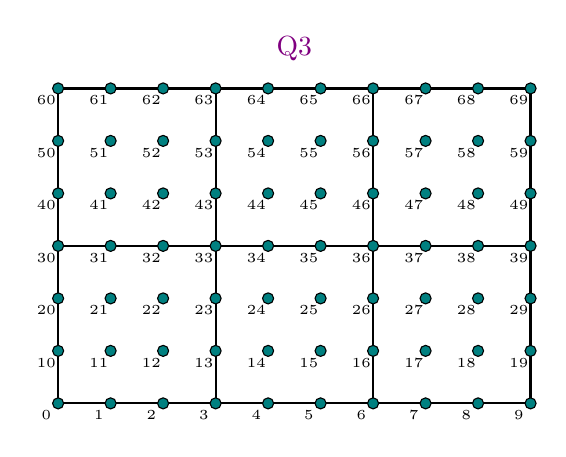
\begin{tikzpicture} 
\node[violet] at (3,4.5) {Q3}; 
\draw[thick] (0,0) -- (6,0) -- (6,4) -- (0,4) -- cycle; 
\draw[thick] (0,2) -- (6,2) ; 
\draw[thick] (2,0) -- (2,4) ; 
\draw[thick] (4,0) -- (4,4) ; 
\draw[black,fill=teal] ( 0.000000 , 0.000000)     circle (2pt); 
\node[] at ( -0.150000, -0.150000 ) {\tiny 0 }; 
\draw[black,fill=teal] ( 0.666667 , 0.000000)     circle (2pt); 
\node[] at ( 0.516667, -0.150000 ) {\tiny 1 }; 
\draw[black,fill=teal] ( 1.333333 , 0.000000)     circle (2pt); 
\node[] at ( 1.183333, -0.150000 ) {\tiny 2 }; 
\draw[black,fill=teal] ( 2.000000 , 0.000000)     circle (2pt); 
\node[] at ( 1.850000, -0.150000 ) {\tiny 3 }; 
\draw[black,fill=teal] ( 2.666667 , 0.000000)     circle (2pt); 
\node[] at ( 2.516667, -0.150000 ) {\tiny 4 }; 
\draw[black,fill=teal] ( 3.333333 , 0.000000)     circle (2pt); 
\node[] at ( 3.183333, -0.150000 ) {\tiny 5 }; 
\draw[black,fill=teal] ( 4.000000 , 0.000000)     circle (2pt); 
\node[] at ( 3.850000, -0.150000 ) {\tiny 6 }; 
\draw[black,fill=teal] ( 4.666667 , 0.000000)     circle (2pt); 
\node[] at ( 4.516667, -0.150000 ) {\tiny 7 }; 
\draw[black,fill=teal] ( 5.333333 , 0.000000)     circle (2pt); 
\node[] at ( 5.183333, -0.150000 ) {\tiny 8 }; 
\draw[black,fill=teal] ( 6.000000 , 0.000000)     circle (2pt); 
\node[] at ( 5.850000, -0.150000 ) {\tiny 9 }; 
\draw[black,fill=teal] ( 0.000000 , 0.666667)     circle (2pt); 
\node[] at ( -0.150000, 0.516667 ) {\tiny 10 }; 
\draw[black,fill=teal] ( 0.666667 , 0.666667)     circle (2pt); 
\node[] at ( 0.516667, 0.516667 ) {\tiny 11 }; 
\draw[black,fill=teal] ( 1.333333 , 0.666667)     circle (2pt); 
\node[] at ( 1.183333, 0.516667 ) {\tiny 12 }; 
\draw[black,fill=teal] ( 2.000000 , 0.666667)     circle (2pt); 
\node[] at ( 1.850000, 0.516667 ) {\tiny 13 }; 
\draw[black,fill=teal] ( 2.666667 , 0.666667)     circle (2pt); 
\node[] at ( 2.516667, 0.516667 ) {\tiny 14 }; 
\draw[black,fill=teal] ( 3.333333 , 0.666667)     circle (2pt); 
\node[] at ( 3.183333, 0.516667 ) {\tiny 15 }; 
\draw[black,fill=teal] ( 4.000000 , 0.666667)     circle (2pt); 
\node[] at ( 3.850000, 0.516667 ) {\tiny 16 }; 
\draw[black,fill=teal] ( 4.666667 , 0.666667)     circle (2pt); 
\node[] at ( 4.516667, 0.516667 ) {\tiny 17 }; 
\draw[black,fill=teal] ( 5.333333 , 0.666667)     circle (2pt); 
\node[] at ( 5.183333, 0.516667 ) {\tiny 18 }; 
\draw[black,fill=teal] ( 6.000000 , 0.666667)     circle (2pt); 
\node[] at ( 5.850000, 0.516667 ) {\tiny 19 }; 
\draw[black,fill=teal] ( 0.000000 , 1.333333)     circle (2pt); 
\node[] at ( -0.150000, 1.183333 ) {\tiny 20 }; 
\draw[black,fill=teal] ( 0.666667 , 1.333333)     circle (2pt); 
\node[] at ( 0.516667, 1.183333 ) {\tiny 21 }; 
\draw[black,fill=teal] ( 1.333333 , 1.333333)     circle (2pt); 
\node[] at ( 1.183333, 1.183333 ) {\tiny 22 }; 
\draw[black,fill=teal] ( 2.000000 , 1.333333)     circle (2pt); 
\node[] at ( 1.850000, 1.183333 ) {\tiny 23 }; 
\draw[black,fill=teal] ( 2.666667 , 1.333333)     circle (2pt); 
\node[] at ( 2.516667, 1.183333 ) {\tiny 24 }; 
\draw[black,fill=teal] ( 3.333333 , 1.333333)     circle (2pt); 
\node[] at ( 3.183333, 1.183333 ) {\tiny 25 }; 
\draw[black,fill=teal] ( 4.000000 , 1.333333)     circle (2pt); 
\node[] at ( 3.850000, 1.183333 ) {\tiny 26 }; 
\draw[black,fill=teal] ( 4.666667 , 1.333333)     circle (2pt); 
\node[] at ( 4.516667, 1.183333 ) {\tiny 27 }; 
\draw[black,fill=teal] ( 5.333333 , 1.333333)     circle (2pt); 
\node[] at ( 5.183333, 1.183333 ) {\tiny 28 }; 
\draw[black,fill=teal] ( 6.000000 , 1.333333)     circle (2pt); 
\node[] at ( 5.850000, 1.183333 ) {\tiny 29 }; 
\draw[black,fill=teal] ( 0.000000 , 2.000000)     circle (2pt); 
\node[] at ( -0.150000, 1.850000 ) {\tiny 30 }; 
\draw[black,fill=teal] ( 0.666667 , 2.000000)     circle (2pt); 
\node[] at ( 0.516667, 1.850000 ) {\tiny 31 }; 
\draw[black,fill=teal] ( 1.333333 , 2.000000)     circle (2pt); 
\node[] at ( 1.183333, 1.850000 ) {\tiny 32 }; 
\draw[black,fill=teal] ( 2.000000 , 2.000000)     circle (2pt); 
\node[] at ( 1.850000, 1.850000 ) {\tiny 33 }; 
\draw[black,fill=teal] ( 2.666667 , 2.000000)     circle (2pt); 
\node[] at ( 2.516667, 1.850000 ) {\tiny 34 }; 
\draw[black,fill=teal] ( 3.333333 , 2.000000)     circle (2pt); 
\node[] at ( 3.183333, 1.850000 ) {\tiny 35 }; 
\draw[black,fill=teal] ( 4.000000 , 2.000000)     circle (2pt); 
\node[] at ( 3.850000, 1.850000 ) {\tiny 36 }; 
\draw[black,fill=teal] ( 4.666667 , 2.000000)     circle (2pt); 
\node[] at ( 4.516667, 1.850000 ) {\tiny 37 }; 
\draw[black,fill=teal] ( 5.333333 , 2.000000)     circle (2pt); 
\node[] at ( 5.183333, 1.850000 ) {\tiny 38 }; 
\draw[black,fill=teal] ( 6.000000 , 2.000000)     circle (2pt); 
\node[] at ( 5.850000, 1.850000 ) {\tiny 39 }; 
\draw[black,fill=teal] ( 0.000000 , 2.666667)     circle (2pt); 
\node[] at ( -0.150000, 2.516667 ) {\tiny 40 }; 
\draw[black,fill=teal] ( 0.666667 , 2.666667)     circle (2pt); 
\node[] at ( 0.516667, 2.516667 ) {\tiny 41 }; 
\draw[black,fill=teal] ( 1.333333 , 2.666667)     circle (2pt); 
\node[] at ( 1.183333, 2.516667 ) {\tiny 42 }; 
\draw[black,fill=teal] ( 2.000000 , 2.666667)     circle (2pt); 
\node[] at ( 1.850000, 2.516667 ) {\tiny 43 }; 
\draw[black,fill=teal] ( 2.666667 , 2.666667)     circle (2pt); 
\node[] at ( 2.516667, 2.516667 ) {\tiny 44 }; 
\draw[black,fill=teal] ( 3.333333 , 2.666667)     circle (2pt); 
\node[] at ( 3.183333, 2.516667 ) {\tiny 45 }; 
\draw[black,fill=teal] ( 4.000000 , 2.666667)     circle (2pt); 
\node[] at ( 3.850000, 2.516667 ) {\tiny 46 }; 
\draw[black,fill=teal] ( 4.666667 , 2.666667)     circle (2pt); 
\node[] at ( 4.516667, 2.516667 ) {\tiny 47 }; 
\draw[black,fill=teal] ( 5.333333 , 2.666667)     circle (2pt); 
\node[] at ( 5.183333, 2.516667 ) {\tiny 48 }; 
\draw[black,fill=teal] ( 6.000000 , 2.666667)     circle (2pt); 
\node[] at ( 5.850000, 2.516667 ) {\tiny 49 }; 
\draw[black,fill=teal] ( 0.000000 , 3.333333)     circle (2pt); 
\node[] at ( -0.150000, 3.183333 ) {\tiny 50 }; 
\draw[black,fill=teal] ( 0.666667 , 3.333333)     circle (2pt); 
\node[] at ( 0.516667, 3.183333 ) {\tiny 51 }; 
\draw[black,fill=teal] ( 1.333333 , 3.333333)     circle (2pt); 
\node[] at ( 1.183333, 3.183333 ) {\tiny 52 }; 
\draw[black,fill=teal] ( 2.000000 , 3.333333)     circle (2pt); 
\node[] at ( 1.850000, 3.183333 ) {\tiny 53 }; 
\draw[black,fill=teal] ( 2.666667 , 3.333333)     circle (2pt); 
\node[] at ( 2.516667, 3.183333 ) {\tiny 54 }; 
\draw[black,fill=teal] ( 3.333333 , 3.333333)     circle (2pt); 
\node[] at ( 3.183333, 3.183333 ) {\tiny 55 }; 
\draw[black,fill=teal] ( 4.000000 , 3.333333)     circle (2pt); 
\node[] at ( 3.850000, 3.183333 ) {\tiny 56 }; 
\draw[black,fill=teal] ( 4.666667 , 3.333333)     circle (2pt); 
\node[] at ( 4.516667, 3.183333 ) {\tiny 57 }; 
\draw[black,fill=teal] ( 5.333333 , 3.333333)     circle (2pt); 
\node[] at ( 5.183333, 3.183333 ) {\tiny 58 }; 
\draw[black,fill=teal] ( 6.000000 , 3.333333)     circle (2pt); 
\node[] at ( 5.850000, 3.183333 ) {\tiny 59 }; 
\draw[black,fill=teal] ( 0.000000 , 4.000000)     circle (2pt); 
\node[] at ( -0.150000, 3.850000 ) {\tiny 60 }; 
\draw[black,fill=teal] ( 0.666667 , 4.000000)     circle (2pt); 
\node[] at ( 0.516667, 3.850000 ) {\tiny 61 }; 
\draw[black,fill=teal] ( 1.333333 , 4.000000)     circle (2pt); 
\node[] at ( 1.183333, 3.850000 ) {\tiny 62 }; 
\draw[black,fill=teal] ( 2.000000 , 4.000000)     circle (2pt); 
\node[] at ( 1.850000, 3.850000 ) {\tiny 63 }; 
\draw[black,fill=teal] ( 2.666667 , 4.000000)     circle (2pt); 
\node[] at ( 2.516667, 3.850000 ) {\tiny 64 }; 
\draw[black,fill=teal] ( 3.333333 , 4.000000)     circle (2pt); 
\node[] at ( 3.183333, 3.850000 ) {\tiny 65 }; 
\draw[black,fill=teal] ( 4.000000 , 4.000000)     circle (2pt); 
\node[] at ( 3.850000, 3.850000 ) {\tiny 66 }; 
\draw[black,fill=teal] ( 4.666667 , 4.000000)     circle (2pt); 
\node[] at ( 4.516667, 3.850000 ) {\tiny 67 }; 
\draw[black,fill=teal] ( 5.333333 , 4.000000)     circle (2pt); 
\node[] at ( 5.183333, 3.850000 ) {\tiny 68 }; 
\draw[black,fill=teal] ( 6.000000 , 4.000000)     circle (2pt); 
\node[] at ( 5.850000, 3.850000 ) {\tiny 69 }; 
\end{tikzpicture} 
\end{center} 


\begin{tiny}
\verbatiminput{python_codes/fieldstone_120/spaces/iconV_elt1_Q3.ascii}
\end{tiny}
\end{multicols}

%------------------
\begin{multicols}{2}
\begin{center} 
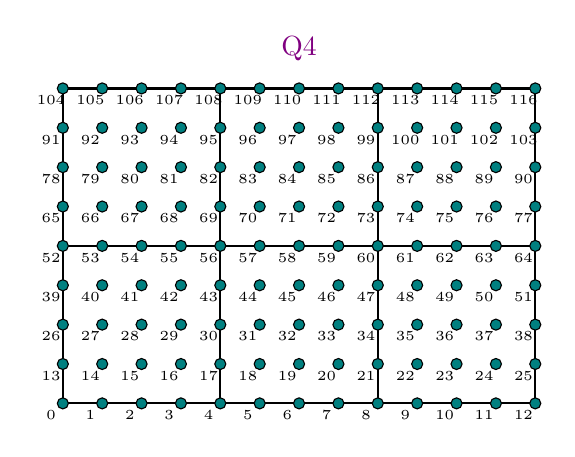
\begin{tikzpicture} 
\node[violet] at (3,4.5) {Q4}; 
\draw[thick] (0,0) -- (6,0) -- (6,4) -- (0,4) -- cycle; 
\draw[thick] (0,2) -- (6,2) ; 
\draw[thick] (2,0) -- (2,4) ; 
\draw[thick] (4,0) -- (4,4) ; 
\draw[black,fill=teal] ( 0.000000 , 0.000000)     circle (2pt); 
\node[] at ( -0.150000, -0.150000 ) {\tiny 0 }; 
\draw[black,fill=teal] ( 0.500000 , 0.000000)     circle (2pt); 
\node[] at ( 0.350000, -0.150000 ) {\tiny 1 }; 
\draw[black,fill=teal] ( 1.000000 , 0.000000)     circle (2pt); 
\node[] at ( 0.850000, -0.150000 ) {\tiny 2 }; 
\draw[black,fill=teal] ( 1.500000 , 0.000000)     circle (2pt); 
\node[] at ( 1.350000, -0.150000 ) {\tiny 3 }; 
\draw[black,fill=teal] ( 2.000000 , 0.000000)     circle (2pt); 
\node[] at ( 1.850000, -0.150000 ) {\tiny 4 }; 
\draw[black,fill=teal] ( 2.500000 , 0.000000)     circle (2pt); 
\node[] at ( 2.350000, -0.150000 ) {\tiny 5 }; 
\draw[black,fill=teal] ( 3.000000 , 0.000000)     circle (2pt); 
\node[] at ( 2.850000, -0.150000 ) {\tiny 6 }; 
\draw[black,fill=teal] ( 3.500000 , 0.000000)     circle (2pt); 
\node[] at ( 3.350000, -0.150000 ) {\tiny 7 }; 
\draw[black,fill=teal] ( 4.000000 , 0.000000)     circle (2pt); 
\node[] at ( 3.850000, -0.150000 ) {\tiny 8 }; 
\draw[black,fill=teal] ( 4.500000 , 0.000000)     circle (2pt); 
\node[] at ( 4.350000, -0.150000 ) {\tiny 9 }; 
\draw[black,fill=teal] ( 5.000000 , 0.000000)     circle (2pt); 
\node[] at ( 4.850000, -0.150000 ) {\tiny 10 }; 
\draw[black,fill=teal] ( 5.500000 , 0.000000)     circle (2pt); 
\node[] at ( 5.350000, -0.150000 ) {\tiny 11 }; 
\draw[black,fill=teal] ( 6.000000 , 0.000000)     circle (2pt); 
\node[] at ( 5.850000, -0.150000 ) {\tiny 12 }; 
\draw[black,fill=teal] ( 0.000000 , 0.500000)     circle (2pt); 
\node[] at ( -0.150000, 0.350000 ) {\tiny 13 }; 
\draw[black,fill=teal] ( 0.500000 , 0.500000)     circle (2pt); 
\node[] at ( 0.350000, 0.350000 ) {\tiny 14 }; 
\draw[black,fill=teal] ( 1.000000 , 0.500000)     circle (2pt); 
\node[] at ( 0.850000, 0.350000 ) {\tiny 15 }; 
\draw[black,fill=teal] ( 1.500000 , 0.500000)     circle (2pt); 
\node[] at ( 1.350000, 0.350000 ) {\tiny 16 }; 
\draw[black,fill=teal] ( 2.000000 , 0.500000)     circle (2pt); 
\node[] at ( 1.850000, 0.350000 ) {\tiny 17 }; 
\draw[black,fill=teal] ( 2.500000 , 0.500000)     circle (2pt); 
\node[] at ( 2.350000, 0.350000 ) {\tiny 18 }; 
\draw[black,fill=teal] ( 3.000000 , 0.500000)     circle (2pt); 
\node[] at ( 2.850000, 0.350000 ) {\tiny 19 }; 
\draw[black,fill=teal] ( 3.500000 , 0.500000)     circle (2pt); 
\node[] at ( 3.350000, 0.350000 ) {\tiny 20 }; 
\draw[black,fill=teal] ( 4.000000 , 0.500000)     circle (2pt); 
\node[] at ( 3.850000, 0.350000 ) {\tiny 21 }; 
\draw[black,fill=teal] ( 4.500000 , 0.500000)     circle (2pt); 
\node[] at ( 4.350000, 0.350000 ) {\tiny 22 }; 
\draw[black,fill=teal] ( 5.000000 , 0.500000)     circle (2pt); 
\node[] at ( 4.850000, 0.350000 ) {\tiny 23 }; 
\draw[black,fill=teal] ( 5.500000 , 0.500000)     circle (2pt); 
\node[] at ( 5.350000, 0.350000 ) {\tiny 24 }; 
\draw[black,fill=teal] ( 6.000000 , 0.500000)     circle (2pt); 
\node[] at ( 5.850000, 0.350000 ) {\tiny 25 }; 
\draw[black,fill=teal] ( 0.000000 , 1.000000)     circle (2pt); 
\node[] at ( -0.150000, 0.850000 ) {\tiny 26 }; 
\draw[black,fill=teal] ( 0.500000 , 1.000000)     circle (2pt); 
\node[] at ( 0.350000, 0.850000 ) {\tiny 27 }; 
\draw[black,fill=teal] ( 1.000000 , 1.000000)     circle (2pt); 
\node[] at ( 0.850000, 0.850000 ) {\tiny 28 }; 
\draw[black,fill=teal] ( 1.500000 , 1.000000)     circle (2pt); 
\node[] at ( 1.350000, 0.850000 ) {\tiny 29 }; 
\draw[black,fill=teal] ( 2.000000 , 1.000000)     circle (2pt); 
\node[] at ( 1.850000, 0.850000 ) {\tiny 30 }; 
\draw[black,fill=teal] ( 2.500000 , 1.000000)     circle (2pt); 
\node[] at ( 2.350000, 0.850000 ) {\tiny 31 }; 
\draw[black,fill=teal] ( 3.000000 , 1.000000)     circle (2pt); 
\node[] at ( 2.850000, 0.850000 ) {\tiny 32 }; 
\draw[black,fill=teal] ( 3.500000 , 1.000000)     circle (2pt); 
\node[] at ( 3.350000, 0.850000 ) {\tiny 33 }; 
\draw[black,fill=teal] ( 4.000000 , 1.000000)     circle (2pt); 
\node[] at ( 3.850000, 0.850000 ) {\tiny 34 }; 
\draw[black,fill=teal] ( 4.500000 , 1.000000)     circle (2pt); 
\node[] at ( 4.350000, 0.850000 ) {\tiny 35 }; 
\draw[black,fill=teal] ( 5.000000 , 1.000000)     circle (2pt); 
\node[] at ( 4.850000, 0.850000 ) {\tiny 36 }; 
\draw[black,fill=teal] ( 5.500000 , 1.000000)     circle (2pt); 
\node[] at ( 5.350000, 0.850000 ) {\tiny 37 }; 
\draw[black,fill=teal] ( 6.000000 , 1.000000)     circle (2pt); 
\node[] at ( 5.850000, 0.850000 ) {\tiny 38 }; 
\draw[black,fill=teal] ( 0.000000 , 1.500000)     circle (2pt); 
\node[] at ( -0.150000, 1.350000 ) {\tiny 39 }; 
\draw[black,fill=teal] ( 0.500000 , 1.500000)     circle (2pt); 
\node[] at ( 0.350000, 1.350000 ) {\tiny 40 }; 
\draw[black,fill=teal] ( 1.000000 , 1.500000)     circle (2pt); 
\node[] at ( 0.850000, 1.350000 ) {\tiny 41 }; 
\draw[black,fill=teal] ( 1.500000 , 1.500000)     circle (2pt); 
\node[] at ( 1.350000, 1.350000 ) {\tiny 42 }; 
\draw[black,fill=teal] ( 2.000000 , 1.500000)     circle (2pt); 
\node[] at ( 1.850000, 1.350000 ) {\tiny 43 }; 
\draw[black,fill=teal] ( 2.500000 , 1.500000)     circle (2pt); 
\node[] at ( 2.350000, 1.350000 ) {\tiny 44 }; 
\draw[black,fill=teal] ( 3.000000 , 1.500000)     circle (2pt); 
\node[] at ( 2.850000, 1.350000 ) {\tiny 45 }; 
\draw[black,fill=teal] ( 3.500000 , 1.500000)     circle (2pt); 
\node[] at ( 3.350000, 1.350000 ) {\tiny 46 }; 
\draw[black,fill=teal] ( 4.000000 , 1.500000)     circle (2pt); 
\node[] at ( 3.850000, 1.350000 ) {\tiny 47 }; 
\draw[black,fill=teal] ( 4.500000 , 1.500000)     circle (2pt); 
\node[] at ( 4.350000, 1.350000 ) {\tiny 48 }; 
\draw[black,fill=teal] ( 5.000000 , 1.500000)     circle (2pt); 
\node[] at ( 4.850000, 1.350000 ) {\tiny 49 }; 
\draw[black,fill=teal] ( 5.500000 , 1.500000)     circle (2pt); 
\node[] at ( 5.350000, 1.350000 ) {\tiny 50 }; 
\draw[black,fill=teal] ( 6.000000 , 1.500000)     circle (2pt); 
\node[] at ( 5.850000, 1.350000 ) {\tiny 51 }; 
\draw[black,fill=teal] ( 0.000000 , 2.000000)     circle (2pt); 
\node[] at ( -0.150000, 1.850000 ) {\tiny 52 }; 
\draw[black,fill=teal] ( 0.500000 , 2.000000)     circle (2pt); 
\node[] at ( 0.350000, 1.850000 ) {\tiny 53 }; 
\draw[black,fill=teal] ( 1.000000 , 2.000000)     circle (2pt); 
\node[] at ( 0.850000, 1.850000 ) {\tiny 54 }; 
\draw[black,fill=teal] ( 1.500000 , 2.000000)     circle (2pt); 
\node[] at ( 1.350000, 1.850000 ) {\tiny 55 }; 
\draw[black,fill=teal] ( 2.000000 , 2.000000)     circle (2pt); 
\node[] at ( 1.850000, 1.850000 ) {\tiny 56 }; 
\draw[black,fill=teal] ( 2.500000 , 2.000000)     circle (2pt); 
\node[] at ( 2.350000, 1.850000 ) {\tiny 57 }; 
\draw[black,fill=teal] ( 3.000000 , 2.000000)     circle (2pt); 
\node[] at ( 2.850000, 1.850000 ) {\tiny 58 }; 
\draw[black,fill=teal] ( 3.500000 , 2.000000)     circle (2pt); 
\node[] at ( 3.350000, 1.850000 ) {\tiny 59 }; 
\draw[black,fill=teal] ( 4.000000 , 2.000000)     circle (2pt); 
\node[] at ( 3.850000, 1.850000 ) {\tiny 60 }; 
\draw[black,fill=teal] ( 4.500000 , 2.000000)     circle (2pt); 
\node[] at ( 4.350000, 1.850000 ) {\tiny 61 }; 
\draw[black,fill=teal] ( 5.000000 , 2.000000)     circle (2pt); 
\node[] at ( 4.850000, 1.850000 ) {\tiny 62 }; 
\draw[black,fill=teal] ( 5.500000 , 2.000000)     circle (2pt); 
\node[] at ( 5.350000, 1.850000 ) {\tiny 63 }; 
\draw[black,fill=teal] ( 6.000000 , 2.000000)     circle (2pt); 
\node[] at ( 5.850000, 1.850000 ) {\tiny 64 }; 
\draw[black,fill=teal] ( 0.000000 , 2.500000)     circle (2pt); 
\node[] at ( -0.150000, 2.350000 ) {\tiny 65 }; 
\draw[black,fill=teal] ( 0.500000 , 2.500000)     circle (2pt); 
\node[] at ( 0.350000, 2.350000 ) {\tiny 66 }; 
\draw[black,fill=teal] ( 1.000000 , 2.500000)     circle (2pt); 
\node[] at ( 0.850000, 2.350000 ) {\tiny 67 }; 
\draw[black,fill=teal] ( 1.500000 , 2.500000)     circle (2pt); 
\node[] at ( 1.350000, 2.350000 ) {\tiny 68 }; 
\draw[black,fill=teal] ( 2.000000 , 2.500000)     circle (2pt); 
\node[] at ( 1.850000, 2.350000 ) {\tiny 69 }; 
\draw[black,fill=teal] ( 2.500000 , 2.500000)     circle (2pt); 
\node[] at ( 2.350000, 2.350000 ) {\tiny 70 }; 
\draw[black,fill=teal] ( 3.000000 , 2.500000)     circle (2pt); 
\node[] at ( 2.850000, 2.350000 ) {\tiny 71 }; 
\draw[black,fill=teal] ( 3.500000 , 2.500000)     circle (2pt); 
\node[] at ( 3.350000, 2.350000 ) {\tiny 72 }; 
\draw[black,fill=teal] ( 4.000000 , 2.500000)     circle (2pt); 
\node[] at ( 3.850000, 2.350000 ) {\tiny 73 }; 
\draw[black,fill=teal] ( 4.500000 , 2.500000)     circle (2pt); 
\node[] at ( 4.350000, 2.350000 ) {\tiny 74 }; 
\draw[black,fill=teal] ( 5.000000 , 2.500000)     circle (2pt); 
\node[] at ( 4.850000, 2.350000 ) {\tiny 75 }; 
\draw[black,fill=teal] ( 5.500000 , 2.500000)     circle (2pt); 
\node[] at ( 5.350000, 2.350000 ) {\tiny 76 }; 
\draw[black,fill=teal] ( 6.000000 , 2.500000)     circle (2pt); 
\node[] at ( 5.850000, 2.350000 ) {\tiny 77 }; 
\draw[black,fill=teal] ( 0.000000 , 3.000000)     circle (2pt); 
\node[] at ( -0.150000, 2.850000 ) {\tiny 78 }; 
\draw[black,fill=teal] ( 0.500000 , 3.000000)     circle (2pt); 
\node[] at ( 0.350000, 2.850000 ) {\tiny 79 }; 
\draw[black,fill=teal] ( 1.000000 , 3.000000)     circle (2pt); 
\node[] at ( 0.850000, 2.850000 ) {\tiny 80 }; 
\draw[black,fill=teal] ( 1.500000 , 3.000000)     circle (2pt); 
\node[] at ( 1.350000, 2.850000 ) {\tiny 81 }; 
\draw[black,fill=teal] ( 2.000000 , 3.000000)     circle (2pt); 
\node[] at ( 1.850000, 2.850000 ) {\tiny 82 }; 
\draw[black,fill=teal] ( 2.500000 , 3.000000)     circle (2pt); 
\node[] at ( 2.350000, 2.850000 ) {\tiny 83 }; 
\draw[black,fill=teal] ( 3.000000 , 3.000000)     circle (2pt); 
\node[] at ( 2.850000, 2.850000 ) {\tiny 84 }; 
\draw[black,fill=teal] ( 3.500000 , 3.000000)     circle (2pt); 
\node[] at ( 3.350000, 2.850000 ) {\tiny 85 }; 
\draw[black,fill=teal] ( 4.000000 , 3.000000)     circle (2pt); 
\node[] at ( 3.850000, 2.850000 ) {\tiny 86 }; 
\draw[black,fill=teal] ( 4.500000 , 3.000000)     circle (2pt); 
\node[] at ( 4.350000, 2.850000 ) {\tiny 87 }; 
\draw[black,fill=teal] ( 5.000000 , 3.000000)     circle (2pt); 
\node[] at ( 4.850000, 2.850000 ) {\tiny 88 }; 
\draw[black,fill=teal] ( 5.500000 , 3.000000)     circle (2pt); 
\node[] at ( 5.350000, 2.850000 ) {\tiny 89 }; 
\draw[black,fill=teal] ( 6.000000 , 3.000000)     circle (2pt); 
\node[] at ( 5.850000, 2.850000 ) {\tiny 90 }; 
\draw[black,fill=teal] ( 0.000000 , 3.500000)     circle (2pt); 
\node[] at ( -0.150000, 3.350000 ) {\tiny 91 }; 
\draw[black,fill=teal] ( 0.500000 , 3.500000)     circle (2pt); 
\node[] at ( 0.350000, 3.350000 ) {\tiny 92 }; 
\draw[black,fill=teal] ( 1.000000 , 3.500000)     circle (2pt); 
\node[] at ( 0.850000, 3.350000 ) {\tiny 93 }; 
\draw[black,fill=teal] ( 1.500000 , 3.500000)     circle (2pt); 
\node[] at ( 1.350000, 3.350000 ) {\tiny 94 }; 
\draw[black,fill=teal] ( 2.000000 , 3.500000)     circle (2pt); 
\node[] at ( 1.850000, 3.350000 ) {\tiny 95 }; 
\draw[black,fill=teal] ( 2.500000 , 3.500000)     circle (2pt); 
\node[] at ( 2.350000, 3.350000 ) {\tiny 96 }; 
\draw[black,fill=teal] ( 3.000000 , 3.500000)     circle (2pt); 
\node[] at ( 2.850000, 3.350000 ) {\tiny 97 }; 
\draw[black,fill=teal] ( 3.500000 , 3.500000)     circle (2pt); 
\node[] at ( 3.350000, 3.350000 ) {\tiny 98 }; 
\draw[black,fill=teal] ( 4.000000 , 3.500000)     circle (2pt); 
\node[] at ( 3.850000, 3.350000 ) {\tiny 99 }; 
\draw[black,fill=teal] ( 4.500000 , 3.500000)     circle (2pt); 
\node[] at ( 4.350000, 3.350000 ) {\tiny 100 }; 
\draw[black,fill=teal] ( 5.000000 , 3.500000)     circle (2pt); 
\node[] at ( 4.850000, 3.350000 ) {\tiny 101 }; 
\draw[black,fill=teal] ( 5.500000 , 3.500000)     circle (2pt); 
\node[] at ( 5.350000, 3.350000 ) {\tiny 102 }; 
\draw[black,fill=teal] ( 6.000000 , 3.500000)     circle (2pt); 
\node[] at ( 5.850000, 3.350000 ) {\tiny 103 }; 
\draw[black,fill=teal] ( 0.000000 , 4.000000)     circle (2pt); 
\node[] at ( -0.150000, 3.850000 ) {\tiny 104 }; 
\draw[black,fill=teal] ( 0.500000 , 4.000000)     circle (2pt); 
\node[] at ( 0.350000, 3.850000 ) {\tiny 105 }; 
\draw[black,fill=teal] ( 1.000000 , 4.000000)     circle (2pt); 
\node[] at ( 0.850000, 3.850000 ) {\tiny 106 }; 
\draw[black,fill=teal] ( 1.500000 , 4.000000)     circle (2pt); 
\node[] at ( 1.350000, 3.850000 ) {\tiny 107 }; 
\draw[black,fill=teal] ( 2.000000 , 4.000000)     circle (2pt); 
\node[] at ( 1.850000, 3.850000 ) {\tiny 108 }; 
\draw[black,fill=teal] ( 2.500000 , 4.000000)     circle (2pt); 
\node[] at ( 2.350000, 3.850000 ) {\tiny 109 }; 
\draw[black,fill=teal] ( 3.000000 , 4.000000)     circle (2pt); 
\node[] at ( 2.850000, 3.850000 ) {\tiny 110 }; 
\draw[black,fill=teal] ( 3.500000 , 4.000000)     circle (2pt); 
\node[] at ( 3.350000, 3.850000 ) {\tiny 111 }; 
\draw[black,fill=teal] ( 4.000000 , 4.000000)     circle (2pt); 
\node[] at ( 3.850000, 3.850000 ) {\tiny 112 }; 
\draw[black,fill=teal] ( 4.500000 , 4.000000)     circle (2pt); 
\node[] at ( 4.350000, 3.850000 ) {\tiny 113 }; 
\draw[black,fill=teal] ( 5.000000 , 4.000000)     circle (2pt); 
\node[] at ( 4.850000, 3.850000 ) {\tiny 114 }; 
\draw[black,fill=teal] ( 5.500000 , 4.000000)     circle (2pt); 
\node[] at ( 5.350000, 3.850000 ) {\tiny 115 }; 
\draw[black,fill=teal] ( 6.000000 , 4.000000)     circle (2pt); 
\node[] at ( 5.850000, 3.850000 ) {\tiny 116 }; 
\end{tikzpicture} 
\end{center} 


\begin{tiny}
\verbatiminput{python_codes/fieldstone_120/spaces/iconV_elt1_Q4.ascii}
\end{tiny}
\end{multicols}

\newpage
%------------------
\begin{multicols}{2}
\begin{center} 
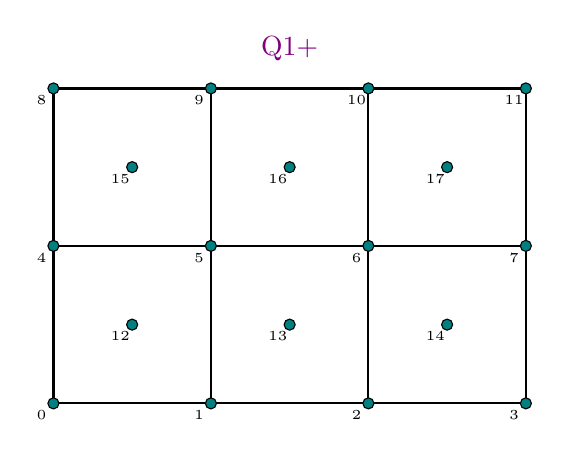
\begin{tikzpicture} 
\node[violet] at (3,4.5) {Q1+}; 
\draw[thick] (0,0) -- (6,0) -- (6,4) -- (0,4) -- cycle; 
\draw[thick] (0,2) -- (6,2) ; 
\draw[thick] (2,0) -- (2,4) ; 
\draw[thick] (4,0) -- (4,4) ; 
\draw[black,fill=teal] ( 0.000000 , 0.000000)     circle (2pt); 
\node[] at ( -0.150000, -0.150000 ) {\tiny 0 }; 
\draw[black,fill=teal] ( 2.000000 , 0.000000)     circle (2pt); 
\node[] at ( 1.850000, -0.150000 ) {\tiny 1 }; 
\draw[black,fill=teal] ( 4.000000 , 0.000000)     circle (2pt); 
\node[] at ( 3.850000, -0.150000 ) {\tiny 2 }; 
\draw[black,fill=teal] ( 6.000000 , 0.000000)     circle (2pt); 
\node[] at ( 5.850000, -0.150000 ) {\tiny 3 }; 
\draw[black,fill=teal] ( 0.000000 , 2.000000)     circle (2pt); 
\node[] at ( -0.150000, 1.850000 ) {\tiny 4 }; 
\draw[black,fill=teal] ( 2.000000 , 2.000000)     circle (2pt); 
\node[] at ( 1.850000, 1.850000 ) {\tiny 5 }; 
\draw[black,fill=teal] ( 4.000000 , 2.000000)     circle (2pt); 
\node[] at ( 3.850000, 1.850000 ) {\tiny 6 }; 
\draw[black,fill=teal] ( 6.000000 , 2.000000)     circle (2pt); 
\node[] at ( 5.850000, 1.850000 ) {\tiny 7 }; 
\draw[black,fill=teal] ( 0.000000 , 4.000000)     circle (2pt); 
\node[] at ( -0.150000, 3.850000 ) {\tiny 8 }; 
\draw[black,fill=teal] ( 2.000000 , 4.000000)     circle (2pt); 
\node[] at ( 1.850000, 3.850000 ) {\tiny 9 }; 
\draw[black,fill=teal] ( 4.000000 , 4.000000)     circle (2pt); 
\node[] at ( 3.850000, 3.850000 ) {\tiny 10 }; 
\draw[black,fill=teal] ( 6.000000 , 4.000000)     circle (2pt); 
\node[] at ( 5.850000, 3.850000 ) {\tiny 11 }; 
\draw[black,fill=teal] ( 1.000000 , 1.000000)     circle (2pt); 
\node[] at ( 0.850000, 0.850000 ) {\tiny 12 }; 
\draw[black,fill=teal] ( 3.000000 , 1.000000)     circle (2pt); 
\node[] at ( 2.850000, 0.850000 ) {\tiny 13 }; 
\draw[black,fill=teal] ( 5.000000 , 1.000000)     circle (2pt); 
\node[] at ( 4.850000, 0.850000 ) {\tiny 14 }; 
\draw[black,fill=teal] ( 1.000000 , 3.000000)     circle (2pt); 
\node[] at ( 0.850000, 2.850000 ) {\tiny 15 }; 
\draw[black,fill=teal] ( 3.000000 , 3.000000)     circle (2pt); 
\node[] at ( 2.850000, 2.850000 ) {\tiny 16 }; 
\draw[black,fill=teal] ( 5.000000 , 3.000000)     circle (2pt); 
\node[] at ( 4.850000, 2.850000 ) {\tiny 17 }; 
\end{tikzpicture} 
\end{center} 


\begin{tiny}
\verbatiminput{python_codes/fieldstone_120/spaces/iconV_elt1_Q1+.ascii}
\end{tiny}
\end{multicols}

%------------------
\begin{multicols}{2}
\begin{center} 
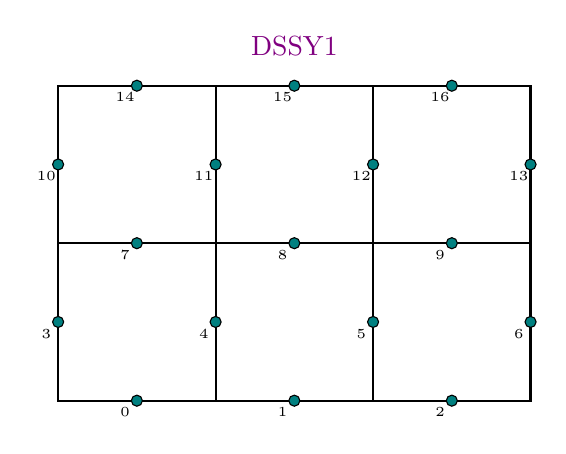
\begin{tikzpicture} 
\node[violet] at (3,4.5) {DSSY1}; 
\draw[thick] (0,0) -- (6,0) -- (6,4) -- (0,4) -- cycle; 
\draw[thick] (0,2) -- (6,2) ; 
\draw[thick] (2,0) -- (2,4) ; 
\draw[thick] (4,0) -- (4,4) ; 
\draw[black,fill=teal] ( 1.000000 , 0.000000)     circle (2pt); 
\node[] at ( 0.850000, -0.150000 ) {\tiny 0 }; 
\draw[black,fill=teal] ( 3.000000 , 0.000000)     circle (2pt); 
\node[] at ( 2.850000, -0.150000 ) {\tiny 1 }; 
\draw[black,fill=teal] ( 5.000000 , 0.000000)     circle (2pt); 
\node[] at ( 4.850000, -0.150000 ) {\tiny 2 }; 
\draw[black,fill=teal] ( 0.000000 , 1.000000)     circle (2pt); 
\node[] at ( -0.150000, 0.850000 ) {\tiny 3 }; 
\draw[black,fill=teal] ( 2.000000 , 1.000000)     circle (2pt); 
\node[] at ( 1.850000, 0.850000 ) {\tiny 4 }; 
\draw[black,fill=teal] ( 4.000000 , 1.000000)     circle (2pt); 
\node[] at ( 3.850000, 0.850000 ) {\tiny 5 }; 
\draw[black,fill=teal] ( 6.000000 , 1.000000)     circle (2pt); 
\node[] at ( 5.850000, 0.850000 ) {\tiny 6 }; 
\draw[black,fill=teal] ( 1.000000 , 2.000000)     circle (2pt); 
\node[] at ( 0.850000, 1.850000 ) {\tiny 7 }; 
\draw[black,fill=teal] ( 3.000000 , 2.000000)     circle (2pt); 
\node[] at ( 2.850000, 1.850000 ) {\tiny 8 }; 
\draw[black,fill=teal] ( 5.000000 , 2.000000)     circle (2pt); 
\node[] at ( 4.850000, 1.850000 ) {\tiny 9 }; 
\draw[black,fill=teal] ( 0.000000 , 3.000000)     circle (2pt); 
\node[] at ( -0.150000, 2.850000 ) {\tiny 10 }; 
\draw[black,fill=teal] ( 2.000000 , 3.000000)     circle (2pt); 
\node[] at ( 1.850000, 2.850000 ) {\tiny 11 }; 
\draw[black,fill=teal] ( 4.000000 , 3.000000)     circle (2pt); 
\node[] at ( 3.850000, 2.850000 ) {\tiny 12 }; 
\draw[black,fill=teal] ( 6.000000 , 3.000000)     circle (2pt); 
\node[] at ( 5.850000, 2.850000 ) {\tiny 13 }; 
\draw[black,fill=teal] ( 1.000000 , 4.000000)     circle (2pt); 
\node[] at ( 0.850000, 3.850000 ) {\tiny 14 }; 
\draw[black,fill=teal] ( 3.000000 , 4.000000)     circle (2pt); 
\node[] at ( 2.850000, 3.850000 ) {\tiny 15 }; 
\draw[black,fill=teal] ( 5.000000 , 4.000000)     circle (2pt); 
\node[] at ( 4.850000, 3.850000 ) {\tiny 16 }; 
\end{tikzpicture} 
\end{center} 


\begin{tiny}
\verbatiminput{python_codes/fieldstone_120/spaces/iconV_elt1_DSSY1.ascii}
\end{tiny}
\end{multicols}

%------------------
%\begin{multicols}{2}
%\begin{center} 
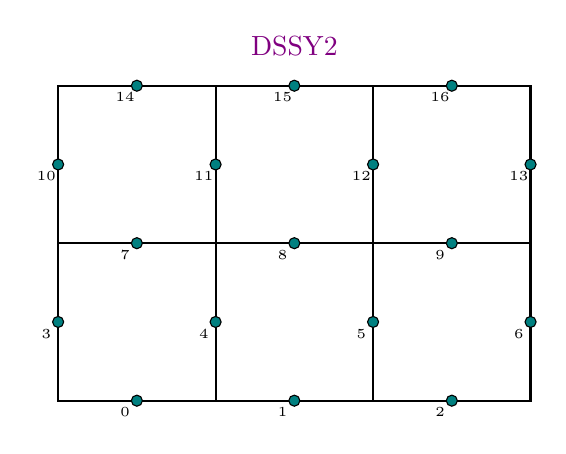
\begin{tikzpicture} 
\node[violet] at (3,4.5) {DSSY2}; 
\draw[thick] (0,0) -- (6,0) -- (6,4) -- (0,4) -- cycle; 
\draw[thick] (0,2) -- (6,2) ; 
\draw[thick] (2,0) -- (2,4) ; 
\draw[thick] (4,0) -- (4,4) ; 
\draw[black,fill=teal] ( 1.000000 , 0.000000)     circle (2pt); 
\node[] at ( 0.850000, -0.150000 ) {\tiny 0 }; 
\draw[black,fill=teal] ( 3.000000 , 0.000000)     circle (2pt); 
\node[] at ( 2.850000, -0.150000 ) {\tiny 1 }; 
\draw[black,fill=teal] ( 5.000000 , 0.000000)     circle (2pt); 
\node[] at ( 4.850000, -0.150000 ) {\tiny 2 }; 
\draw[black,fill=teal] ( 0.000000 , 1.000000)     circle (2pt); 
\node[] at ( -0.150000, 0.850000 ) {\tiny 3 }; 
\draw[black,fill=teal] ( 2.000000 , 1.000000)     circle (2pt); 
\node[] at ( 1.850000, 0.850000 ) {\tiny 4 }; 
\draw[black,fill=teal] ( 4.000000 , 1.000000)     circle (2pt); 
\node[] at ( 3.850000, 0.850000 ) {\tiny 5 }; 
\draw[black,fill=teal] ( 6.000000 , 1.000000)     circle (2pt); 
\node[] at ( 5.850000, 0.850000 ) {\tiny 6 }; 
\draw[black,fill=teal] ( 1.000000 , 2.000000)     circle (2pt); 
\node[] at ( 0.850000, 1.850000 ) {\tiny 7 }; 
\draw[black,fill=teal] ( 3.000000 , 2.000000)     circle (2pt); 
\node[] at ( 2.850000, 1.850000 ) {\tiny 8 }; 
\draw[black,fill=teal] ( 5.000000 , 2.000000)     circle (2pt); 
\node[] at ( 4.850000, 1.850000 ) {\tiny 9 }; 
\draw[black,fill=teal] ( 0.000000 , 3.000000)     circle (2pt); 
\node[] at ( -0.150000, 2.850000 ) {\tiny 10 }; 
\draw[black,fill=teal] ( 2.000000 , 3.000000)     circle (2pt); 
\node[] at ( 1.850000, 2.850000 ) {\tiny 11 }; 
\draw[black,fill=teal] ( 4.000000 , 3.000000)     circle (2pt); 
\node[] at ( 3.850000, 2.850000 ) {\tiny 12 }; 
\draw[black,fill=teal] ( 6.000000 , 3.000000)     circle (2pt); 
\node[] at ( 5.850000, 2.850000 ) {\tiny 13 }; 
\draw[black,fill=teal] ( 1.000000 , 4.000000)     circle (2pt); 
\node[] at ( 0.850000, 3.850000 ) {\tiny 14 }; 
\draw[black,fill=teal] ( 3.000000 , 4.000000)     circle (2pt); 
\node[] at ( 2.850000, 3.850000 ) {\tiny 15 }; 
\draw[black,fill=teal] ( 5.000000 , 4.000000)     circle (2pt); 
\node[] at ( 4.850000, 3.850000 ) {\tiny 16 }; 
\end{tikzpicture} 
\end{center} 


%\begin{tiny}
%\verbatiminput{python_codes/fieldstone_120/spaces/iconV_elt1_DSSY2.ascii}
%\end{tiny}
%\end{multicols}

%------------------
\begin{multicols}{2}
\begin{center} 
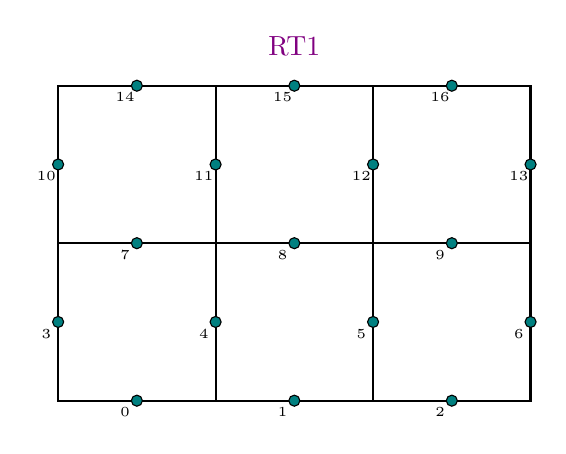
\begin{tikzpicture} 
\node[violet] at (3,4.5) {RT1}; 
\draw[thick] (0,0) -- (6,0) -- (6,4) -- (0,4) -- cycle; 
\draw[thick] (0,2) -- (6,2) ; 
\draw[thick] (2,0) -- (2,4) ; 
\draw[thick] (4,0) -- (4,4) ; 
\draw[black,fill=teal] ( 1.000000 , 0.000000)     circle (2pt); 
\node[] at ( 0.850000, -0.150000 ) {\tiny 0 }; 
\draw[black,fill=teal] ( 3.000000 , 0.000000)     circle (2pt); 
\node[] at ( 2.850000, -0.150000 ) {\tiny 1 }; 
\draw[black,fill=teal] ( 5.000000 , 0.000000)     circle (2pt); 
\node[] at ( 4.850000, -0.150000 ) {\tiny 2 }; 
\draw[black,fill=teal] ( 0.000000 , 1.000000)     circle (2pt); 
\node[] at ( -0.150000, 0.850000 ) {\tiny 3 }; 
\draw[black,fill=teal] ( 2.000000 , 1.000000)     circle (2pt); 
\node[] at ( 1.850000, 0.850000 ) {\tiny 4 }; 
\draw[black,fill=teal] ( 4.000000 , 1.000000)     circle (2pt); 
\node[] at ( 3.850000, 0.850000 ) {\tiny 5 }; 
\draw[black,fill=teal] ( 6.000000 , 1.000000)     circle (2pt); 
\node[] at ( 5.850000, 0.850000 ) {\tiny 6 }; 
\draw[black,fill=teal] ( 1.000000 , 2.000000)     circle (2pt); 
\node[] at ( 0.850000, 1.850000 ) {\tiny 7 }; 
\draw[black,fill=teal] ( 3.000000 , 2.000000)     circle (2pt); 
\node[] at ( 2.850000, 1.850000 ) {\tiny 8 }; 
\draw[black,fill=teal] ( 5.000000 , 2.000000)     circle (2pt); 
\node[] at ( 4.850000, 1.850000 ) {\tiny 9 }; 
\draw[black,fill=teal] ( 0.000000 , 3.000000)     circle (2pt); 
\node[] at ( -0.150000, 2.850000 ) {\tiny 10 }; 
\draw[black,fill=teal] ( 2.000000 , 3.000000)     circle (2pt); 
\node[] at ( 1.850000, 2.850000 ) {\tiny 11 }; 
\draw[black,fill=teal] ( 4.000000 , 3.000000)     circle (2pt); 
\node[] at ( 3.850000, 2.850000 ) {\tiny 12 }; 
\draw[black,fill=teal] ( 6.000000 , 3.000000)     circle (2pt); 
\node[] at ( 5.850000, 2.850000 ) {\tiny 13 }; 
\draw[black,fill=teal] ( 1.000000 , 4.000000)     circle (2pt); 
\node[] at ( 0.850000, 3.850000 ) {\tiny 14 }; 
\draw[black,fill=teal] ( 3.000000 , 4.000000)     circle (2pt); 
\node[] at ( 2.850000, 3.850000 ) {\tiny 15 }; 
\draw[black,fill=teal] ( 5.000000 , 4.000000)     circle (2pt); 
\node[] at ( 4.850000, 3.850000 ) {\tiny 16 }; 
\end{tikzpicture} 
\end{center} 


\begin{tiny}
\verbatiminput{python_codes/fieldstone_120/spaces/iconV_elt1_RT1.ascii}
\end{tiny}
\end{multicols}

%------------------
%\begin{multicols}{2}
%\begin{center} 
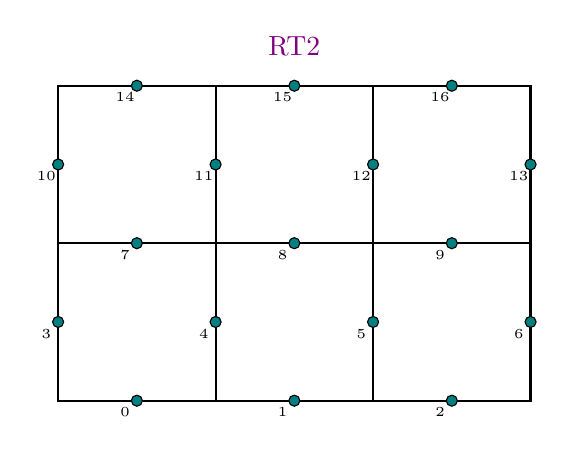
\begin{tikzpicture} 
\node[violet] at (3,4.5) {RT2}; 
\draw[thick] (0,0) -- (6,0) -- (6,4) -- (0,4) -- cycle; 
\draw[thick] (0,2) -- (6,2) ; 
\draw[thick] (2,0) -- (2,4) ; 
\draw[thick] (4,0) -- (4,4) ; 
\draw[black,fill=teal] ( 1.000000 , 0.000000)     circle (2pt); 
\node[] at ( 0.850000, -0.150000 ) {\tiny 0 }; 
\draw[black,fill=teal] ( 3.000000 , 0.000000)     circle (2pt); 
\node[] at ( 2.850000, -0.150000 ) {\tiny 1 }; 
\draw[black,fill=teal] ( 5.000000 , 0.000000)     circle (2pt); 
\node[] at ( 4.850000, -0.150000 ) {\tiny 2 }; 
\draw[black,fill=teal] ( 0.000000 , 1.000000)     circle (2pt); 
\node[] at ( -0.150000, 0.850000 ) {\tiny 3 }; 
\draw[black,fill=teal] ( 2.000000 , 1.000000)     circle (2pt); 
\node[] at ( 1.850000, 0.850000 ) {\tiny 4 }; 
\draw[black,fill=teal] ( 4.000000 , 1.000000)     circle (2pt); 
\node[] at ( 3.850000, 0.850000 ) {\tiny 5 }; 
\draw[black,fill=teal] ( 6.000000 , 1.000000)     circle (2pt); 
\node[] at ( 5.850000, 0.850000 ) {\tiny 6 }; 
\draw[black,fill=teal] ( 1.000000 , 2.000000)     circle (2pt); 
\node[] at ( 0.850000, 1.850000 ) {\tiny 7 }; 
\draw[black,fill=teal] ( 3.000000 , 2.000000)     circle (2pt); 
\node[] at ( 2.850000, 1.850000 ) {\tiny 8 }; 
\draw[black,fill=teal] ( 5.000000 , 2.000000)     circle (2pt); 
\node[] at ( 4.850000, 1.850000 ) {\tiny 9 }; 
\draw[black,fill=teal] ( 0.000000 , 3.000000)     circle (2pt); 
\node[] at ( -0.150000, 2.850000 ) {\tiny 10 }; 
\draw[black,fill=teal] ( 2.000000 , 3.000000)     circle (2pt); 
\node[] at ( 1.850000, 2.850000 ) {\tiny 11 }; 
\draw[black,fill=teal] ( 4.000000 , 3.000000)     circle (2pt); 
\node[] at ( 3.850000, 2.850000 ) {\tiny 12 }; 
\draw[black,fill=teal] ( 6.000000 , 3.000000)     circle (2pt); 
\node[] at ( 5.850000, 2.850000 ) {\tiny 13 }; 
\draw[black,fill=teal] ( 1.000000 , 4.000000)     circle (2pt); 
\node[] at ( 0.850000, 3.850000 ) {\tiny 14 }; 
\draw[black,fill=teal] ( 3.000000 , 4.000000)     circle (2pt); 
\node[] at ( 2.850000, 3.850000 ) {\tiny 15 }; 
\draw[black,fill=teal] ( 5.000000 , 4.000000)     circle (2pt); 
\node[] at ( 4.850000, 3.850000 ) {\tiny 16 }; 
\end{tikzpicture} 
\end{center} 


%\begin{tiny}
%\verbatiminput{python_codes/fieldstone_120/spaces/iconV_elt1_RT2.ascii}
%\end{tiny}
%\end{multicols}

%------------------
\begin{multicols}{2}
\begin{center} 
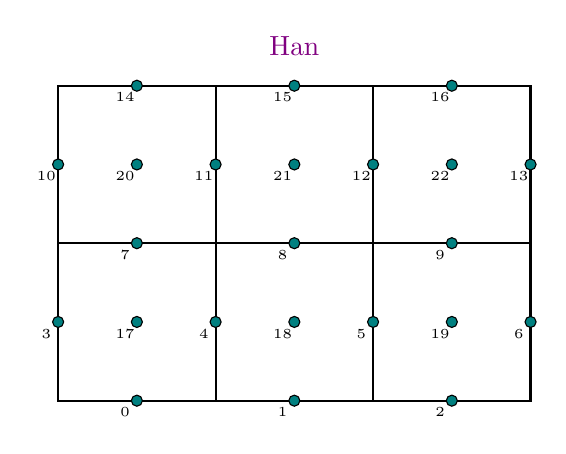
\begin{tikzpicture} 
\node[violet] at (3,4.5) {Han}; 
\draw[thick] (0,0) -- (6,0) -- (6,4) -- (0,4) -- cycle; 
\draw[thick] (0,2) -- (6,2) ; 
\draw[thick] (2,0) -- (2,4) ; 
\draw[thick] (4,0) -- (4,4) ; 
\draw[black,fill=teal] ( 1.000000 , 0.000000)     circle (2pt); 
\node[] at ( 0.850000, -0.150000 ) {\tiny 0 }; 
\draw[black,fill=teal] ( 3.000000 , 0.000000)     circle (2pt); 
\node[] at ( 2.850000, -0.150000 ) {\tiny 1 }; 
\draw[black,fill=teal] ( 5.000000 , 0.000000)     circle (2pt); 
\node[] at ( 4.850000, -0.150000 ) {\tiny 2 }; 
\draw[black,fill=teal] ( 0.000000 , 1.000000)     circle (2pt); 
\node[] at ( -0.150000, 0.850000 ) {\tiny 3 }; 
\draw[black,fill=teal] ( 2.000000 , 1.000000)     circle (2pt); 
\node[] at ( 1.850000, 0.850000 ) {\tiny 4 }; 
\draw[black,fill=teal] ( 4.000000 , 1.000000)     circle (2pt); 
\node[] at ( 3.850000, 0.850000 ) {\tiny 5 }; 
\draw[black,fill=teal] ( 6.000000 , 1.000000)     circle (2pt); 
\node[] at ( 5.850000, 0.850000 ) {\tiny 6 }; 
\draw[black,fill=teal] ( 1.000000 , 2.000000)     circle (2pt); 
\node[] at ( 0.850000, 1.850000 ) {\tiny 7 }; 
\draw[black,fill=teal] ( 3.000000 , 2.000000)     circle (2pt); 
\node[] at ( 2.850000, 1.850000 ) {\tiny 8 }; 
\draw[black,fill=teal] ( 5.000000 , 2.000000)     circle (2pt); 
\node[] at ( 4.850000, 1.850000 ) {\tiny 9 }; 
\draw[black,fill=teal] ( 0.000000 , 3.000000)     circle (2pt); 
\node[] at ( -0.150000, 2.850000 ) {\tiny 10 }; 
\draw[black,fill=teal] ( 2.000000 , 3.000000)     circle (2pt); 
\node[] at ( 1.850000, 2.850000 ) {\tiny 11 }; 
\draw[black,fill=teal] ( 4.000000 , 3.000000)     circle (2pt); 
\node[] at ( 3.850000, 2.850000 ) {\tiny 12 }; 
\draw[black,fill=teal] ( 6.000000 , 3.000000)     circle (2pt); 
\node[] at ( 5.850000, 2.850000 ) {\tiny 13 }; 
\draw[black,fill=teal] ( 1.000000 , 4.000000)     circle (2pt); 
\node[] at ( 0.850000, 3.850000 ) {\tiny 14 }; 
\draw[black,fill=teal] ( 3.000000 , 4.000000)     circle (2pt); 
\node[] at ( 2.850000, 3.850000 ) {\tiny 15 }; 
\draw[black,fill=teal] ( 5.000000 , 4.000000)     circle (2pt); 
\node[] at ( 4.850000, 3.850000 ) {\tiny 16 }; 
\draw[black,fill=teal] ( 1.000000 , 1.000000)     circle (2pt); 
\node[] at ( 0.850000, 0.850000 ) {\tiny 17 }; 
\draw[black,fill=teal] ( 3.000000 , 1.000000)     circle (2pt); 
\node[] at ( 2.850000, 0.850000 ) {\tiny 18 }; 
\draw[black,fill=teal] ( 5.000000 , 1.000000)     circle (2pt); 
\node[] at ( 4.850000, 0.850000 ) {\tiny 19 }; 
\draw[black,fill=teal] ( 1.000000 , 3.000000)     circle (2pt); 
\node[] at ( 0.850000, 2.850000 ) {\tiny 20 }; 
\draw[black,fill=teal] ( 3.000000 , 3.000000)     circle (2pt); 
\node[] at ( 2.850000, 2.850000 ) {\tiny 21 }; 
\draw[black,fill=teal] ( 5.000000 , 3.000000)     circle (2pt); 
\node[] at ( 4.850000, 2.850000 ) {\tiny 22 }; 
\end{tikzpicture} 
\end{center} 


\begin{tiny}
\verbatiminput{python_codes/fieldstone_120/spaces/iconV_elt1_Han.ascii}
\end{tiny}
\end{multicols}




\newpage
%-----------------------------------------------------------------------------
\subsection*{Python testers}

\begin{itemize}
\item \lstinline{tester1.py}: checks that each basis function is 1 on its support node and zero at all other nodes.
\item \lstinline{tester2.py}: computes the area of each element by means of numerical quadrature. The domain is 3x2 and there are 3x2 elements so that we expect 1 for quadrilateral elements and 0.5 for triangular elements.  
\item \lstinline{tester3.py}: computes the space derivatives of each coordinate minus one, so that we expect zero (down to machine precision). It returns 'passed' if the results is less than $10^{-12}$.   
\item \lstinline{tester4.py}: computes the gradient of $x^2/2$ and $y^2/2$ (i.e. resp. $x$ and $y$) to which the coordinate of the quadrature point is subtracted so that one expect zero again. This test can only be passed by quadratic and higher order elements.
\item \lstinline{tester5.py}: produces 3x2 tikz files and corresponding iconV files. 
\item \lstinline{tester6.py}: produces pdf files of reference elements.
\end{itemize}


\newpage
%-----------------------------------------------------------------------------
\subsection*{Pressure normalisation for augmented Taylor-Hood elements}


I tried both ${\bm P}_2\times (P_1+P_0)$ and ${\bm Q}_2\times (Q_1+Q_0)$ on different manufactured solutions 
and I observed for both that the pressure I obtained visually consisted of 2 fields: (for quads) 
the continuous $Q_1$ which looked similar to the expected analytical field although offset by what 
seemed a constant (bottom green points), and the $Q_0$ field (top green points) which was 
very different than the $Q_1$ pressure:

\begin{center}
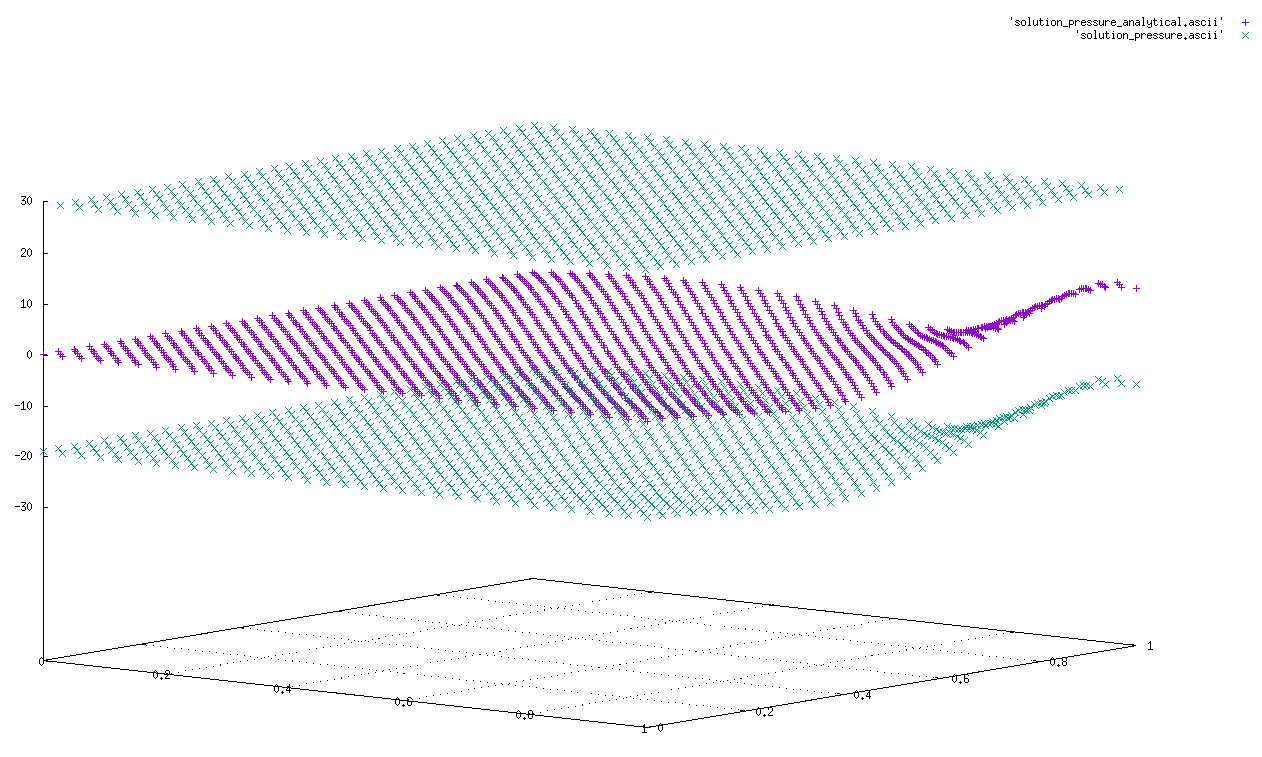
\includegraphics[width=8cm]{python_codes/fieldstone_120/images/q2q1q0pb}
\end{center}

I of course make sure in my code that the pressure fulfills $\int p dV=0$ but since 
the global constant function $p=constant$ is both in the $Q_1$ and $Q_0$ spaces the 
resulting normalised pressure was never good (see green line on plot below). 
This got me thinking about the '2 hydrostatic modes' of Gresho \& Sani and
I ended up looking at pressure normalisation in the following way (for quads again):
\begin{eqnarray}
0 
&=& \int_\Omega p dV \nn\\
&=& \sum_e \int_{\Omega_e} p dV \nn\\
&=& \sum_e \int_{\Omega_e} \left( \sum_{i=1}^5 \bN_i(x,y) p_i \right) dV \nn\\
&=& \sum_e \int_{\Omega_e} \left( \sum_{i=1}^4 \bN_i(x,y) p_i + \bN_5 p_5 \right) dV
\end{eqnarray}
with $\bN_{1,2,3,4}(r,s)=\frac14(1\pm r)(1\pm s)$ being
the $Q_1$ basis functions, $p_{1,2,3,4}$ the pressures at the corners
of the quad and $\bN_5(r,s)=1$ the $Q_0$ basis functions with $p_5$ the elemental pressure.
I then obtain 
\begin{eqnarray}
0 
&=& \underbrace{\sum_e \int_{\Omega_e} \left( \sum_{i=1}^4 \bN_i(x,y) p_i \right) dV}_{<p>_{Q_1}}
+ \underbrace{\sum_e \int_{\Omega_e} p_5  dV}_{<p>_{Q_0}}
\end{eqnarray}
and proceed to normalise the pressure by imposing both $<p>_{Q_1}=0$ and $<p>_{Q_0}=0$.
In this case the 'doubly normalised' pressure agrees with the analytical solution 
and I obtain the following error convergence plot:

\begin{center}
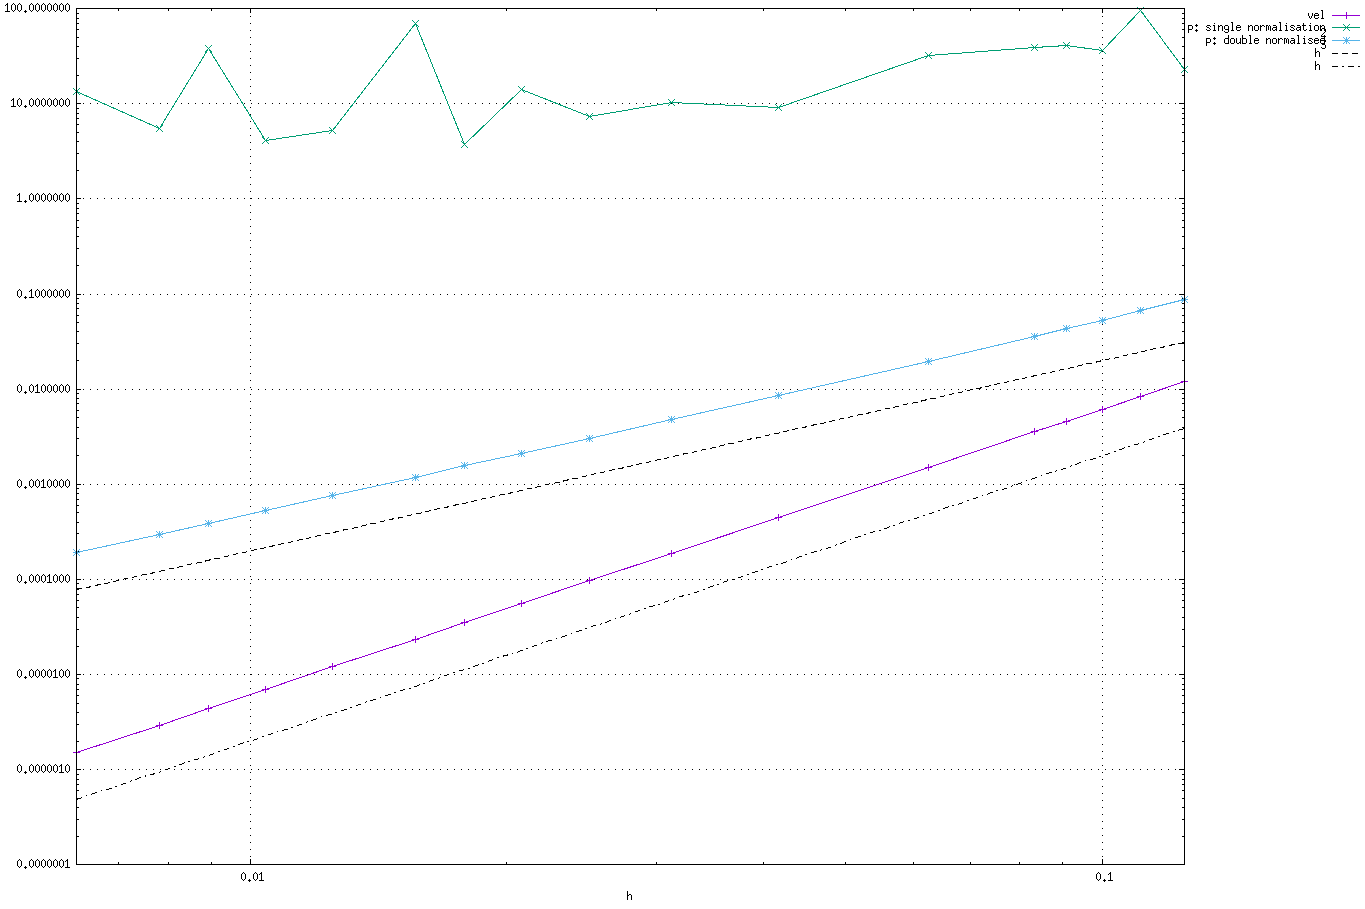
\includegraphics[width=8cm]{python_codes/fieldstone_120/images/q2q1q0}\\
{\captionfont 'doubly normalised' pressure error convergence is quadratic (blue line) and 
velocity error convergence is cubic (purple line). The green line is the 'wrong/raw' pressure. }
\end{center}




\newpage
%-----------------------------------------------------------------------------
\subsection*{Breakdown of the code}

One starts by loading the required finite element functions 
for the basis functions, the numerical quadrature and various tools:
\begin{lstlisting}
import FEbasis2D as FE
import FEquadrature as Q
import FEtools as Tools 
\end{lstlisting}

Then the desired setup/manufacture solution is imported, say:
\begin{lstlisting}
import mms_jolm17 as mms
\end{lstlisting}


The domain is a unit square:
\begin{lstlisting}
Lx=1
Ly=1
\end{lstlisting}

It is discretised by means of a $nelx\times nely$ cells. If quadrilateral 
elements are to be used then there are $nelx\times nely$ elements. If 
triangular elements are to be used then the cells are cut into two 
triangles and there are then $2\times nelx\times nely$ elements.

\begin{lstlisting}
nelx=16
nely=16
\end{lstlisting}

%There are four boundaries to the domain (left, right, bottom and top). For the 
%benchmark under consideration we need to impose no slip boundary conditions 
%on all sides of the domain:
%\begin{lstlisting}
%left_bc  ='no_slip'
%right_bc ='no_slip'
%bottom_bc='no_slip'
%top_bc   ='no_slip'
%\end{lstlisting}

In two dimensions there are two velocity degrees of freedom per 
velocity node but only one pressure degree of freedom per pressure node:
\begin{lstlisting}
ndofV=2
ndofP=1
\end{lstlisting}

A finite element space must be assigned to both velocity and pressure. For example: 
\begin{lstlisting}
Vspace='Q2'
Pspace='Q1'
\end{lstlisting}

Whether a (bi-)linear mapping or isoparametric mapping is used is set with 
this parameter:
\begin{lstlisting}
isoparametric=False
\end{lstlisting}

Whether the mesh is randominzed or not is set with 
\begin{lstlisting}
randomize_mesh=True
\end{lstlisting}


A quadrature order must be assigned. If quadrilateral elements are used
this parameter is the number of quadrature points per dimension. 
If triangular elements are used it is the total number of quadrature points 
inside the element. For example: 
\begin{lstlisting}
nqpts=Q.nqpts_default(Vpsace)
\end{lstlisting}

For the chosen velocity and pressure spaces we retrieve the number of nodes 
('support points') inside an element.
\begin{lstlisting}
mV=FE.NNN_m(Vspace)
mP=FE.NNN_m(Pspace)
\end{lstlisting}

We then setup the quadrature rule for an element. This function 
returns the number of quadrature points inside the element, 
their coordinates in the $r,s$ space and their weights: 
\begin{lstlisting}
nqel,qcoords_r,qcoords_s,qweights=Q.quadrature(Vspace,nqpts)
\end{lstlisting}

The mesh is then created, or rather the meshes: one for the 
velocity nodes, one for the pressure nodes. They both count the 
same number of elements. There are \lstinline{NV} velocity nodes and their
coordinates are stored in the \lstinline{xV} and \lstinline{yV} arrays.
Likewise there are \lstinline{NP} pressure nodes and their
coordinates are stored in the \lstinline{xP} and \lstinline{yP} arrays. 

\begin{lstlisting}
NV,nel,xV,yV,iconV=Tools.cartesian_mesh(Lx,Ly,nelx,nely,Vspace)
NP,nel,xP,yP,iconP=Tools.cartesian_mesh(Lx,Ly,nelx,nely,Pspace)
\end{lstlisting}

Now that we know the number of elements and nodes we can compute the 
total number of quadrature points \lstinline{nq}, 
the total number of velocity dofs \lstinline{NfemV}, 
the total number of pressure dofs \lstinline{NfemP}, 
and the total number of dofs:

\begin{lstlisting}
nq=nqel*nel
NfemV=NV*ndofV
NfemP=NP*ndofP
Nfem=NfemV+NfemP
\end{lstlisting}

We will later need two arrays of size \lstinline{NfemV} (we are only imposing
velocity boundary conditions). \lstinline{bc_fix} is a boolean array.
We set \lstinline{bc_fix[i]=True} if the value of a given velocity dof \lstinline{i} is set. 
and the value of \lstinline{bc_val[i]} is the value of the desired boundary condition.

\begin{lstlisting}
bc_fix,bc_val=Tools.bc_setup(xV,yV,Lx,Ly,ndofV,mms.left_bc,mms.right_bc,mms.bottom_bc,mms.top_bc)
\end{lstlisting}

We then build the background mesh used for the mapping:
\begin{lstlisting}
space1=FE.mapping(Vspace)
m1=FE.NNN_m(space1)
N1,nel1,x1,y1,icon1=Tools.cartesian_mesh(Lx,Ly,nelx,nely,space1)
if randomize_mesh:
   Tools.randomize_background_mesh(x1,y1,hx,hy,N1,Lx,Ly)
   Tools.adapt_FE_mesh(x1,y1,icon1,m1,space1,xV,yV,iconV,nel,Vspace)
   Tools.adapt_FE_mesh(x1,y1,icon1,m1,space1,xP,yP,iconP,nel,Pspace)
\end{lstlisting}




Then we proceed to compute the volume of each element, i.e. 
\[
V_e = \int_{\Omega_e} dV = \sum_{iq=1}^{n_q} \omega_{i_q} |J_{i_q}|
\]
which translates as follows: 
\begin{lstlisting}
for iel in range(0,nel):
  for iq in range(0,nqel):
    rq=qcoords_r[iq]
    sq=qcoords_s[iq]
    weightq=qweights[iq]
    NNNV=FE.NNN(rq,sq,Vspace)
    dNNNVdr=FE.dNNNdr(rq,sq,Vspace)
    dNNNVds=FE.dNNNds(rq,sq,Vspace)
    jcob,jcbi,dNNNVdx,dNNNVdy=Tools.J(mV,dNNNVdr,dNNNVds,xV[iconV[0:mV,iel]],yV[iconV[0:mV,iel]])
    area[iel]+=jcob*weightq
\end{lstlisting}

FINISH!!!


\newpage
%%%%%%%%%%%%%%%%%%%%%%%%%%%%%%%%%%%%%%%%%%%%%%%%%%%%%%%%%%%%%%%%%%%%%%%%%%%%%%%
\section*{Results - mms from John's book}

It is derived in Section~\ref{ss:mms_johnbook}. The velocity and pressure fields are:
\begin{eqnarray}
u(x,y) &=& 1000 x^2(1-x)^4  y^2 (3-5y) (1-y) \\
v(x,y) &=& -1000 2x(1-3x) (1-x)^3  y^3(1-y)^2   \\
p(x,y) &=& \pi^2 [xy^3 \cos(2\pi x^2 y) - x^2y \sin(2\pi xy) ]+1/8
\end{eqnarray}

\begin{center}
\includegraphics[width=8cm]{python_codes/fieldstone_120/results_johnbook/errors-velocity-all}
\includegraphics[width=8cm]{python_codes/fieldstone_120/results_johnbook/errors-pressure-all}\\
\includegraphics[width=8cm]{python_codes/fieldstone_120/results_johnbook/errors-divv-all}
\includegraphics[width=8cm]{python_codes/fieldstone_120/results_johnbook/vrms_zoom}
\end{center}


\begin{center} 
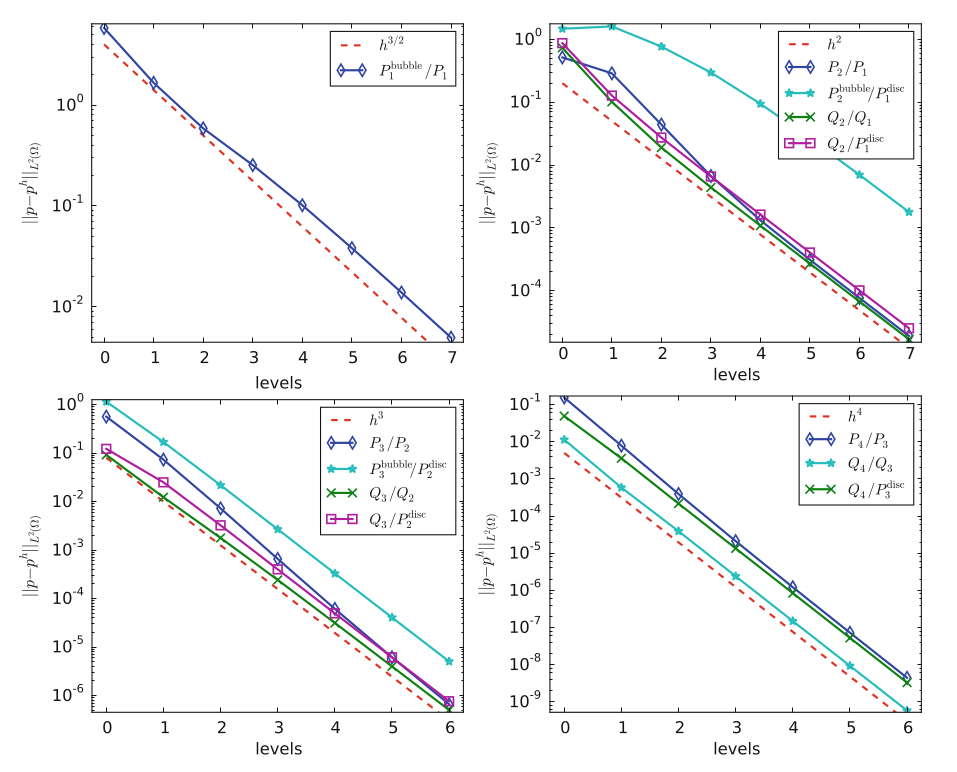
\includegraphics[width=8.5cm]{python_codes/fieldstone_120/images/john_a}
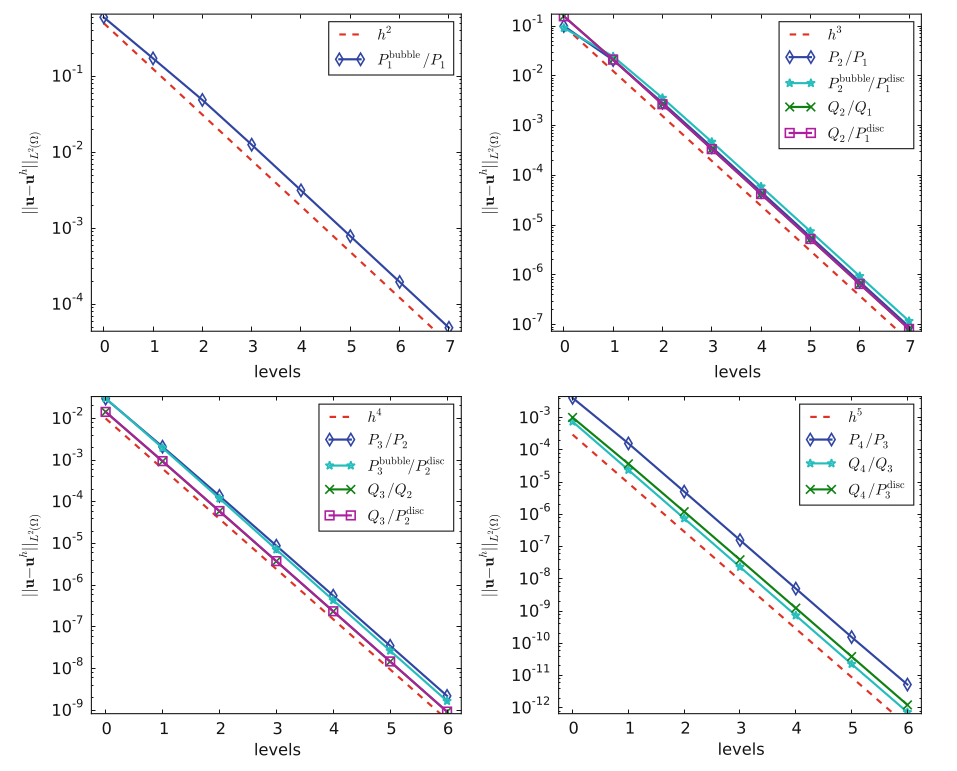
\includegraphics[width=8.5cm]{python_codes/fieldstone_120/images/john_b}\\
{\captionfont Taken from \textcite{john16} (book).}
\end{center} 

\newpage
%%%%%%%%%%%%%%%%%%%%%%%%%%%%%%%%%%%%%%%%%%%%%%%%%%%%%%%%%%%%%%%%%%%%%%%%%%%%%%%
\section*{Results - \textcite{jolm17} manufactured solution}

This benchmark comes from John \etal \cite{jolm17} and is presented in Section~\ref{ss:mms_jolm17}:
\begin{eqnarray}
u(x,y) &=& 200x^2(1-x)^2y(1-y)(1-2y) \nn\\
v(x,y) &=& -200x(1-x)(1-2x)y^2(1-y)^2 \nn\\
p(x,y) &=& 10\left[(x-1/2)^3y^2+(1-x)^3(y-1/2)^3 \right] \nn
\end{eqnarray}
The highest polynomial terms for the velocity are quartic and cubic for the pressure.


\begin{center}
\includegraphics[width=8cm]{python_codes/fieldstone_120/results_jolm17/errors-velocity-all}
\includegraphics[width=8cm]{python_codes/fieldstone_120/results_jolm17/errors-pressure-all}\\
\includegraphics[width=8cm]{python_codes/fieldstone_120/results_jolm17/errors-divv-all}
\includegraphics[width=8cm]{python_codes/fieldstone_120/results_jolm17/vrms_zoom}
\end{center}

%1----------------------------
\subsection*{$Q_1\times Q_0$}
\begin{center}
\includegraphics[width=8cm]{python_codes/fieldstone_120/results/Q1Q0-vp-h.pdf}
\includegraphics[width=8cm]{python_codes/fieldstone_120/results/Q1Q0-vp-Nfem.pdf}
\end{center}

%2----------------------------
\subsection*{$Q_2\times Q_0$}
\begin{center}
\includegraphics[width=8cm]{python_codes/fieldstone_120/results/Q2Q0-vp-h.pdf}
\includegraphics[width=8cm]{python_codes/fieldstone_120/results/Q2Q0-vp-Nfem.pdf}
\end{center}

%3----------------------------
\subsection*{$P_2\times P_0$}
\begin{center}
\includegraphics[width=8cm]{python_codes/fieldstone_120/results/P2P0-vp-h.pdf}
\includegraphics[width=8cm]{python_codes/fieldstone_120/results/P2P0-vp-Nfem.pdf}
\end{center}

%4----------------------------
\subsection*{$Q_2\times Q_1$}
\begin{center}
\includegraphics[width=8cm]{python_codes/fieldstone_120/results/Q2Q1-vp-h.pdf}
\includegraphics[width=8cm]{python_codes/fieldstone_120/results/Q2Q1-vp-Nfem.pdf}
\end{center}

%5----------------------------
\subsection*{$P_2\times P_1$}
\begin{center}
\includegraphics[width=8cm]{python_codes/fieldstone_120/results/P2P1-vp-h.pdf}
\includegraphics[width=8cm]{python_codes/fieldstone_120/results/P2P1-vp-Nfem.pdf}
\end{center}

%6----------------------------
\subsection*{$Q_3\times Q_2$}
\begin{center}
\includegraphics[width=8cm]{python_codes/fieldstone_120/results/Q3Q2-vp-h.pdf}
\includegraphics[width=8cm]{python_codes/fieldstone_120/results/Q3Q2-vp-Nfem.pdf}
\end{center}

%7----------------------------
\subsection*{$P_3\times P_2$}
\begin{center}
\includegraphics[width=8cm]{python_codes/fieldstone_120/results/P3P2-vp-h.pdf}
\includegraphics[width=8cm]{python_codes/fieldstone_120/results/P3P2-vp-Nfem.pdf}
\end{center}

\newpage
%8----------------------------
\subsection*{$Q_1^+\times Q_1$}
\begin{center}
\includegraphics[width=8cm]{python_codes/fieldstone_120/results/Q1+Q1-vp-h.pdf}
\includegraphics[width=8cm]{python_codes/fieldstone_120/results/Q1+Q1-vp-Nfem.pdf}
\end{center}

%9----------------------------
\subsection*{$P_1^+\times P_1$}
\begin{center}
\includegraphics[width=8cm]{python_codes/fieldstone_120/results/P1+P1-vp-h.pdf}
\includegraphics[width=8cm]{python_codes/fieldstone_120/results/P1+P1-vp-Nfem.pdf}
\end{center}

%10----------------------------
\subsection*{$RT_1\times Q_0$}
\begin{center}
\includegraphics[width=8cm]{python_codes/fieldstone_120/results/RT1Q0-vp-h.pdf}
\includegraphics[width=8cm]{python_codes/fieldstone_120/results/RT1Q0-vp-Nfem.pdf}
\end{center}

%11----------------------------
\subsection*{$RT_2\times Q_0$}
\begin{center}
\includegraphics[width=8cm]{python_codes/fieldstone_120/results/RT2Q0-vp-h.pdf}
\includegraphics[width=8cm]{python_codes/fieldstone_120/results/RT2Q0-vp-Nfem.pdf}
\end{center}

%12----------------------------
\subsection*{$DSSY_1\times Q_0$}
\begin{center}
\includegraphics[width=8cm]{python_codes/fieldstone_120/results/DSSY1Q0-vp-h.pdf}
\includegraphics[width=8cm]{python_codes/fieldstone_120/results/DSSY1Q0-vp-Nfem.pdf}
\end{center}

%13----------------------------
\subsection*{$DSSY_2\times Q_0$}
\begin{center}
\includegraphics[width=8cm]{python_codes/fieldstone_120/results/DSSY2Q0-vp-h.pdf}
\includegraphics[width=8cm]{python_codes/fieldstone_120/results/DSSY2Q0-vp-Nfem.pdf}
\end{center}

%14----------------------------
\subsection*{$Han\times Q_0$}
\begin{center}
\includegraphics[width=8cm]{python_codes/fieldstone_120/results/HanQ0-vp-h.pdf}
\includegraphics[width=8cm]{python_codes/fieldstone_120/results/HanQ0-vp-Nfem.pdf}
\end{center}

%15----------------------------
\subsection*{$Q_2\times P_{-1}$}
\begin{center}
\includegraphics[width=8cm]{python_codes/fieldstone_120/results/Q2Pm1-vp-h.pdf}
\includegraphics[width=8cm]{python_codes/fieldstone_120/results/Q2Pm1-vp-Nfem.pdf}
\end{center}

%16----------------------------
\subsection*{$Q_2\times P_{-1}(u)$}
\begin{center}
\includegraphics[width=8cm]{python_codes/fieldstone_120/results/Q2Pm1u-vp-h.pdf}
\includegraphics[width=8cm]{python_codes/fieldstone_120/results/Q2Pm1u-vp-Nfem.pdf}
\end{center}

%17----------------------------
\subsection*{$Q_2^{(8)}\times Q_1$}
\begin{center}
\includegraphics[width=8cm]{python_codes/fieldstone_120/results/Q2sQ1-vp-h.pdf}
\includegraphics[width=8cm]{python_codes/fieldstone_120/results/Q2sQ1-vp-Nfem.pdf}
\end{center}

%18----------------------------
\subsection*{$P_2^+\times P_{-1}$}
\begin{center}
\includegraphics[width=8cm]{python_codes/fieldstone_120/results/P2+P-1-vp-h.pdf}
\includegraphics[width=8cm]{python_codes/fieldstone_120/results/P2+P-1-vp-Nfem.pdf}
\end{center}

%19----------------------------
\subsection*{$P_2^+\times P_{1}$}
\begin{center}
\includegraphics[width=8cm]{python_codes/fieldstone_120/results/P2+P1-vp-h.pdf}
\includegraphics[width=8cm]{python_codes/fieldstone_120/results/P2+P1-vp-Nfem.pdf}
\end{center}



\newpage
optimal quadrature \& convergence orders:

\begin{center}
\begin{tabular}{l|ccc|ccc|}
\hline
                     & d\&h &   & vj3 & \\
                     & nq &v    & nq & p & v & p \\
\hline
\hline
$Q_1\times Q_0$       & 2    & X & 2 & X  \\%1
$Q_2\times Q_0$       &     &  &  &       \\%2
$P_2\times Q_0$       &     &  &  &       \\%3
$Q_2\times Q_1$       &      &   & 3 & 2  \\%4 
$P_2\times P_1$       &      &   & 3 & 2  \\%5
$Q_3\times Q_2$       &      &   & 4 & 3  \\%6
$P_3\times P_2$       &      &   & 4 & 3  \\%7
$Q_1^+\times Q_1$     &      &   & 2 & {\bf 1.5}  \\%8
$P_1^+\times P_{1}$   &      &   & 2 & {\bf 1.5}  \\%9
$RT_1\times Q_0$      &      &   & 2 & 1(?)\\%10
$RT_2\times Q_0$      &      &   & 2 & 1   \\%11
$DSSY_1\times Q_0$    &      &   & 2 & 1   \\%12
$DSSY_2\times Q_0$    &      &   & 2 & 1   \\%13
$Han\times Q_0$       &      &   & 2 & 1   \\%14
$Q_2\times P_{-1}$    &      &   & 3 & 2   \\%15
$Q_2\times P_{-1}(u)$ &      &   &  &      \\%16
$Q_2^{(8)}\times Q_1$ &      &   & 3 & 2   \\%17
$P_2^+\times P_{-1}$  &      &   & 3 & 2   \\%18
$P_2^+\times P_{1}$   &      &   & 3 & 2   \\%19
\hline
\end{tabular} 
\end{center}

\vspace{1cm}

Conclusions:
\begin{itemize}
\item $Q_1\times Q_0$ pressure is plagued by checkeboard mode (nothing new, won't be included in paper anyways)
\item P1+P1 and Q1+Q1 exhibit the same convergence order: 2 for velocity and 1.5 for pressure.
\item compare Q2Q1 and Q2P-1
\item compare Q2Q1 and Q28Q1
\item P2P0 vel convergence not cubic ?
\end{itemize}






\newpage
%%%%%%%%%%%%%%%%%%%%%%%%%%%%%%%%%%%%%%%%%%%%%%%%%%%%%%%%%%%%%%%%%%%%%%%%%%%%%%%
\section*{Results - square sinker}

Unit square. Free-slip boundary conditions. domain filled with fluid with $\eta_f=1$ and $\rho_f=1$.
Square sinker in the middle of the domain of size $0.25\times 0.25$ with $\eta_s=100$ and
$\rho_s=1.001$. Gravity is $\vec{g}=-\vec{e}_y$. 
%Resolutions nelx=8, 16, 32, 64, 128 
%are chosen so that element boundaries align with sinker boundaries 
%(material averaging is irrelevant). 

There is no analytical solution so by setting $\vec{\upnu}^{th}=\vec{0}$ and 
$p^{th}=0$ the computed errors are in fact the vrms and prms shown hereunder.

\begin{center}
\includegraphics[width=6cm]{python_codes/fieldstone_120/results_sinker/velocity}
\includegraphics[width=6cm]{python_codes/fieldstone_120/results_sinker/pressure}\\
{\captionfont Velocity and pressure field on $64\times 64$ mesh of $Q_2\times Q_1$ elements.}
\end{center}

\begin{center}
\includegraphics[width=8cm]{python_codes/fieldstone_120/results_sinker/errors-velocity-all}
\includegraphics[width=8cm]{python_codes/fieldstone_120/results_sinker/errors-pressure-all}\\
\includegraphics[width=8cm]{python_codes/fieldstone_120/results_sinker/errors-divv-all}
\includegraphics[width=8cm]{python_codes/fieldstone_120/results_sinker/vrms_zoom}
\end{center}



%\begin{center}
%\includegraphics[width=8.5cm]{python_codes/fieldstone_120/results_sinker/errors-velocity-all}
%\includegraphics[width=8.5cm]{python_codes/fieldstone_120/results_sinker/errors-velocity-subset}\\
%\includegraphics[width=8.5cm]{python_codes/fieldstone_120/results_sinker/errors-pressure-all}
%\includegraphics[width=8.5cm]{python_codes/fieldstone_120/results_sinker/errors-pressure-subset}\\
%{\captionfont We find that the DSSY and RT elements yield very abnormal results at low resolution
%so they are removed from the plots in the right column. The prms of the regular $Q_1\times Q_0$ element 
%is also removed.}
%\end{center}

conclusion:

\begin{itemize}
\item DSSY, RT and Han elements are not usable for buoyancy-driven flows in the presence of a hydrostatic 
background. Their velocity is all over the place, but their pressure seems to very slowly 
converge at high resolution to the pressure of the other elements.
RETRIEVE email correspondance with Rannacher! show velocity field modes. Has smthg to do with 
Korn stuff.
\end{itemize}

\newpage
%%%%%%%%%%%%%%%%%%%%%%%%%%%%%%%%%%%%%%%%%%%%%%%%%%%%%%%%%%%%%%%%%%%%%%%%%%%%%%%
\section*{Results - shear flow}

\newpage
TODO:

Write code which computes null space of G 

randomize mesh

write function in FEtools with interpolates v and p on point ?

mms with nonzero dirichlet bc?

Korn inequality something ?



Remaining questions/ideas:

- no flow benchmark ? i.e bent downwards 2D domain. 

- compute jcb, jci, jcob for 3x2 with all elements.

- should I implement edge stab - dG stuff for R-T elements ? if not they should be  
removed from study. Probably same with Han and Chen.

Remark:

- P1NC-P0, MINI, BR and P2P0 compared on mms in \cite{cakp15}

- check jolm17 results

